\documentclass[12pt,american]{article}

\usepackage[T1]{fontenc}
\usepackage[utf8]{inputenc}
\usepackage{authblk}
\usepackage{xcolor}
\usepackage{booktabs,siunitx}
\usepackage{multirow}
\usepackage{lscape}
\usepackage{tabularx}
\usepackage{natbib}
\usepackage{geometry}
\usepackage{amsmath}
\usepackage{amssymb}
\usepackage{booktabs,caption}
\usepackage[flushleft]{threeparttable}
\usepackage{makecell}
\usepackage{setspace}
\usepackage{xspace}[2006/05/08]
\usepackage{subcaption}
\usepackage{multicol} 
\usepackage{paralist} 
\captionsetup[subtable]{labelformat=simple, labelsep=colon}
\renewcommand{\thesubtable}{Panel~\Alph{subtable}}  
\sisetup{input-decimal-markers = {.}} 
%%%%%%%%%%%%%%%%%%%%%%%%%%%%%%%%%%%%%%% CODE
\usepackage{listings}
\usepackage{xparse} 
%%%%%% FORMATTING CODE OUTPUT
\definecolor{codebackground}{rgb}{0.95, 0.95, 0.92}
\definecolor{userbackground}{RGB}{252,255,233}
\lstset{language=C,
        keywordstyle={\bfseries \color{blue}},
        backgroundcolor  = \color{codebackground},
        keepspaces       = true,
        basicstyle       = {\ttfamily\footnotesize},
        numbers=left,
        numberstyle      = \scriptsize\color{black},
        numbersep        = 5pt,
        frame=tb, 
        breaklines=true
}
\newcommand{\commandtex}[1]{\textcolor{blue}{#1}\@\xspace}
% Define VHDL style
\lstdefinestyle{vhdlStyle}{
  language=VHDL,
  basicstyle=\ttfamily\footnotesize,
  keywordstyle=\color{blue},
  commentstyle=\color{green!50!black},
  stringstyle=\color{red},
  breaklines=true,
  showstringspaces=false,
  morekeywords={library, use, all, entity, is, port, in, out, end, architecture, of, begin, and, or, if, then, else, elsif, process, signal, assign}
}
\usepackage{threeparttable}
\usepackage{multibib}
\newcites{app}{Appendix References}

%%%%%%%%%%%%%%%%%%%%%%%%%%%%%%%%%%%%%%% CEIL FUNCTION
\usepackage{mathtools}
\DeclarePairedDelimiter\ceil{\lceil}{\rceil}
\DeclarePairedDelimiter\floor{\lfloor}{\rfloor}
%%%%%%%%%%%%%%%%%%%%%%%%%%%%%%
\usepackage[breaklinks]{hyperref}
\hypersetup{
    colorlinks = true,
    linkcolor=blue,
    citecolor=red,
    urlcolor=cyan
    }
\geometry{verbose,left=5.4em, right=5.4em, top=5.4em, bottom=5.4em}
\renewcommand\Authands{ and }
\usepackage{atbegshi}
\AtBeginDocument{\AtBeginShipoutNext{\AtBeginShipoutDiscard}}
%%%%%%%%%%%%%%%%%%%%%%%%%%%%%%%%%%%%%%%%%%%%%%%%%%%%%%%%%%%%%%%%%%%%%%%%%%%%%%%%%%%
%                           USER-DEFINED COMMANDS
%%%%%%%%%%%%%%%%%%%%%%%%%%%%%%%%%%%%%%%%%%%%%%%%%%%%%%%%%%%%%%%%%%%%%%%%%%%%%%%%%%%
%%%%%%%%%%%%%%%%%%%%%%%%% NOTATION
\newcommand{\kprime}{k^{\prime}}
\newcommand{\kdis}{\mathbf{\Gamma}}
\newcommand{\kupd}{\widehat{k}'_{i+1}}
\newcommand{\kgss}{\kprime_{i}}
\newcommand{\tollk}{\varepsilon_{k}}
\newcommand{\kopt}{k^{\prime}}
\newcommand{\Aset}{\mathbf{A}}
\newcommand{\kset}{\mathbf{K}}
\newcommand{\idset}{\{0,1\}_{\epsilon}}
\newcommand{\kdismom}{m}
\newcommand{\kdismomset}{\mathbf{M}}
\newcommand{\lbar}{\bar{l}}
\newcommand{\Leff}{\lbar L}
\newcommand{\state}{k,\epsilon,m,A}
\newcommand{\stateset}{\kset \times \idset \times \kdismomset \times \Aset}
\newcommand{\KGRID}{\bar{K}}
\newcommand{\MGRID}{\bar{M}}
\newcommand{\mprime}{m^{\prime}}
\newcommand{\bhat}{\hat{b_i}}
\newcommand{\Naccsize}{J}
%%%%%%%%%%%%%%%%%%%%%%% RESULTS FOLDERS AND NAMING
\newcommand{\resultsfolder}{./results}
\newcommand{\graphicsfolder}{./graphics}
\newcommand{\devfpgaI}{fpgaI}
\newcommand{\devfpgaII}{fpgaII}
\newcommand{\devfpgaIII}{fpgaIII}
\newcommand{\devcpu}{cpu-cores}
\newcommand{\nKMIkI}{nKM4-nk100}
\newcommand{\nKMIkII}{nKM4-nk200}
\newcommand{\nKMIkIII}{nKM4-nk300}
\newcommand{\nKMIIkI}{nKM8-nk100}
\newcommand{\nKMIIkII}{nKM8-nk200}
\newcommand{\nKMIIkIII}{nKM8-nk300}
\newcommand{\knlI}{knl-1}
\newcommand{\knlII}{knl-3}
%%%%%%%%%%%%%%%%%%%%%%%%%%%%%%%%%%%%%%%%
% Instances
\newcommand{\cpuI}{m5n.large\@\xspace}
\newcommand{\cpucoreI}{1}   
\newcommand{\cpucostI}{0.119}  
\newcommand{\cpuII}{m5n.4xlarge\@\xspace}
\newcommand{\cpucoreII}{8}  
\newcommand{\cpucostII}{0.952}  
\newcommand{\cpuIII}{m5n.24xlarge\@\xspace}
\newcommand{\cpucoreIII}{48} 
\newcommand{\cpucostIII}{5.712}  
\newcommand{\awsinstI}{\textcolor{magenta}{z1d.2xlarge}\@\xspace}
\newcommand{\awsinstcostI}{\textcolor{magenta}{0.744}\@\xspace}
\newcommand{\awsinstfI}{f1.2xlarge\@\xspace}
\newcommand{\awsinstcostfI}{\textcolor{magenta}{1.65}\@\xspace}
\newcommand{\awsinstfII}{f1.4xlarge\@\xspace}
\newcommand{\awsinstcostfII}{\textcolor{magenta}{3.30}\@\xspace}
\newcommand{\awsinstfIII}{f1.16xlarge\@\xspace}
\newcommand{\awsinstcostfIII}{\textcolor{magenta}{13.20}\@\xspace}

%%%%%%%%%%%%%%%%% Abstract
\newcommand{\baselinespeedupFPGAICPUI}{\input{\resultsfolder/cpu-cores1-fpgaI-nKM4-nk100-speedup_rounded.txt}\@\xspace} 
\newcommand{\cpuItimehoursminutes}{\input{\resultsfolder/cpu-cores1-nKM4-nk100-hours_rounded.txt} hours\@\xspace}     
\newcommand{\fpgaItimehoursminutes}{\input{\resultsfolder/fpgaI-nKM4-nk100-minutes_rounded.txt} minutes\@\xspace}  
%%%%%%%%%%%%%%%%% Introduction
\newcommand{\baselinespeedupFPGAICPUIII}{\input{\resultsfolder/cpu-cores48-fpgaI-nKM4-nk100-speedup.txt}} 
\newcommand{\baselinespeedupFPGAIIICPUI}{\input{\resultsfolder/cpu-cores1-fpgaIII-nKM4-nk100-speedup_rounded.txt}} 
\newcommand{\baselinespeedupFPGAIIICPUII}{\input{\resultsfolder/cpu-cores8-fpgaIII-nKM4-nk100-speedup_rounded.txt}} 
\newcommand{\baselinespeedupFPGAIIICPUIII}{\input{\resultsfolder/cpu-cores48-fpgaIII-nKM4-nk100-speedup_rounded.txt}} 
\newcommand{\costupperbound}{\input{\resultsfolder/maxcostsavings_rounded.txt}} 
\newcommand{\energyupperbound}{\input{\resultsfolder/maxenergysavings_rounded.txt}} 
%%%%%%%%%%%%%%%%% Quantitative Results
%%%%%%%%%%%%%%%%%%%%% Section: Speedups of FPGA 
\newcommand{\cpuIItimehoursminutes}{approximately \input{\resultsfolder/cpu-cores8-nKM4-nk100-hours_rounded.txt} hour\@\xspace}     
% Costs
\newcommand{\CPUcostonemillioneconomies}{\$\input{\resultsfolder/cpu-cores1-nKM4-nk100-cost-million_economies.txt}}
\newcommand{\FPGAcostonemillioneconomies}{\$\input{\resultsfolder/fpgaI-nKM4-nk100-cost-million_economies.txt}\@\xspace}
%%%%%%%%%%%%%%%%%%%%% Section: Robustness
\newcommand{\THEORETICALspeedupFPGAICPUI}{\input{\resultsfolder/cpu-cores1-fpgaI-nKM4-nk100-speedup-theoretical.txt}} 
\newcommand{\fpgaIknlIpowerconsumption}{\input{\resultsfolder/carbfoot_fpgaI-knl-1-nKM4-nk100-power.txt}}
%%%%%%%%%%%%%%%%% Inspecting the Mechanism > Baseline
\newcommand{\avgfpgaIbasenKMIkItime}{\input{\resultsfolder/fpgaI-base-knl-1-nKM4-nk100-time-avg_rounded.txt}}
 \newcommand{\avgcpubasenKMIkItime}{\input{\resultsfolder/cpu-cores1-nKM4-nk100-time-avg_rounded.txt}}
\newcommand{\avgfpgacpusbasespeedup}{\input{\resultsfolder/cpu-cores1-fpgaI-knl-1-base-nKM4-nk100-speedup-word.txt}times slower than}
%%%%%%%%%%%%%%%%%%%%% Section: Inspecting the Mechanism > Within-Data Parallelism 
\newcommand{\fpgaIdatparknlISimulationSteptime}{\input{\resultsfolder/fpgaI-knl-1-nKM4-nk100-sim-time-tot.txt}\hspace{-0.12cm}ms}
\newcommand{\fpgaIdatparknlIIAPSteptime}{\input{\resultsfolder/fpgaI-knl-1-nKM4-nk100-ihp-time-tot.txt}\hspace{-0.12cm}ms}
\newcommand{\fpgaIdatparknlISimulationStepspeedup}{\input{\resultsfolder/cpu-cores1-fpgaI-knl-1-nKM4-nk100-speedup-sim.txt}\hspace{-0.12cm}x}
\newcommand{\fpgaIdatparknlIIAPStepspeedup}{\input{\resultsfolder/cpu-cores1-fpgaI-knl-1-nKM4-nk100-speedup-ihp.txt}\hspace{-0.12cm}x}
 %%%%%%%%%%%%%%%%% Carbon Footprint
 \newcommand{\fpgaIpowerconsumption}{\input{\resultsfolder/carbfoot_fpgaI-nKM4-nk100-power.txt}}
\newcommand{\fpgaIpowerconsumptionperhour}{\input{\resultsfolder/carbfoot_fpgaI-nKM4-nk100-power_kWh.txt}}
\newcommand{\fpgaICOIIpoundsperhour}{\input{\resultsfolder/carbfoot_lbsC02_fpgahour.txt}}
\newcommand{\SummitonFPGAtothours}{\input{\resultsfolder/carbfoot_Summit_yearlyhour_on_fpga.txt}}
\newcommand{\SummitonFPGAtotlbsCOII}{\input{\resultsfolder/carbfoot_lbsC02_year.txt}}
\newcommand{\SummitonFPGAtotmTonCOII}{\input{\resultsfolder/carbfoot_metrictonsC02_year.txt}}
\newcommand{\fpgacars}{\input{\resultsfolder/carbfoot_cars_fpga_word.txt}}
\newcommand{\fpgacarsnumber}{\input{\resultsfolder/carbfoot_cars_fpga.txt}}
%%%%%%%%%%%%%%%%%%%%%%%%%%%%%%%%%%%%%%%%%%%%%%%%%%%%%%%%%%%%%%%%%%%%%%%%%%%%%%%%%%%
%                           AUTOMATIC UPDATE TABLES
%%%%%%%%%%%%%%%%%%%%%%%%%%%%%%%%%%%%%%%%%%%%%%%%%%%%%%%%%%%%%%%%%%%%%%%%%%%%%%%%%%%
%%%%%%%%%%%%%%%%%%%% TABLE 2: Benchmarking the C code
\newcommand{\cpulineartime}{\input{\resultsfolder/\devcpu\cpucoreI-linear-kernel-time.txt}}
\newcommand{\cpubinarytime}{\input{\resultsfolder/\devcpu\cpucoreI-binary-kernel-time.txt}}
\newcommand{\cpujumpsearchtime}{\input{\resultsfolder/\devcpu\cpucoreI-\nKMIkI-kernel-time.txt}}
\newcommand{\cpubinaryspeedup}{\input{\resultsfolder/\devcpu\cpucoreI-binary-speedup.txt}}
\newcommand{\cpujumpsearchspeedup}{\input{\resultsfolder/\devcpu\cpucoreI-jumpsearch-speedup.txt}}
%%%%%%%%%%%%%%%%%%%% TABLE A4: Three-Kernel Comparison: Time, Cost, Energy
\newcommand{\cpuItimetot}{\input{\resultsfolder/\devcpu\cpucoreI-\nKMIkI-time-tot.txt}}
\newcommand{\cpuIinittime}{\input{\resultsfolder/\devcpu\cpucoreI-\nKMIkI-init-time.txt}}
\newcommand{\cpuIwritetime}{\input{\resultsfolder/\devcpu\cpucoreI-\nKMIkI-write-time.txt}}
\newcommand{\cpuItime}{\input{\resultsfolder/\devcpu\cpucoreI-\nKMIkI-kernel-time.txt}}
\newcommand{\cpuIcost}{\input{\resultsfolder/\devcpu\cpucoreI-\nKMIkI-cost.txt}}
\newcommand{\cpuIenergy}{\input{\resultsfolder/\devcpu\cpucoreI-\nKMIkI-energy.txt}}
\newcommand{\cpuIItimetot}{\input{\resultsfolder/\devcpu\cpucoreII-\nKMIkI-time-tot.txt}}
\newcommand{\cpuIIinittime}{\input{\resultsfolder/\devcpu\cpucoreII-\nKMIkI-init-time.txt}}
\newcommand{\cpuIIwritetime}{\input{\resultsfolder/\devcpu\cpucoreII-\nKMIkI-write-time.txt}}
\newcommand{\cpuIItime}{\input{\resultsfolder/\devcpu\cpucoreII-\nKMIkI-kernel-time.txt}}
\newcommand{\cpuIIcost}{\input{\resultsfolder/\devcpu\cpucoreII-\nKMIkI-cost.txt}}
\newcommand{\cpuIIenergy}{\input{\resultsfolder/\devcpu\cpucoreII-\nKMIkI-energy.txt}}
\newcommand{\cpuIIItimetot}{\input{\resultsfolder/\devcpu\cpucoreIII-\nKMIkI-time-tot.txt}}
\newcommand{\cpuIIIinittime}{\input{\resultsfolder/\devcpu\cpucoreIII-\nKMIkI-init-time.txt}}
\newcommand{\cpuIIIwritetime}{\input{\resultsfolder/\devcpu\cpucoreIII-\nKMIkI-write-time.txt}}
\newcommand{\cpuIIItime}{\input{\resultsfolder/\devcpu\cpucoreIII-\nKMIkI-kernel-time.txt}}
\newcommand{\cpuIIIcost}{\input{\resultsfolder/\devcpu\cpucoreIII-\nKMIkI-cost.txt}}
\newcommand{\cpuIIIenergy}{\input{\resultsfolder/\devcpu\cpucoreIII-\nKMIkI-energy.txt}}
\newcommand{\fpgaItimetot}{\input{\resultsfolder/\devfpgaI-\nKMIkI-time-tot.txt}}
\newcommand{\fpgaIinittime}{\input{\resultsfolder/\devfpgaI-\nKMIkI-init-time.txt}}
\newcommand{\fpgaIwritetime}{\input{\resultsfolder/\devfpgaI-\nKMIkI-write-time.txt}}
\newcommand{\fpgaItime}{\input{\resultsfolder/\devfpgaI-\nKMIkI-kernel-time.txt}}
\newcommand{\fpgaIcost}{\input{\resultsfolder/\devfpgaI-\nKMIkI-cost.txt}}
\newcommand{\fpgaIenergy}{\input{\resultsfolder/\devfpgaI-\nKMIkI-energy.txt}}
\newcommand{\fpgaIItimetot}{\input{\resultsfolder/\devfpgaII-\nKMIkI-time-tot.txt}}
\newcommand{\fpgaIIinittime}{\input{\resultsfolder/\devfpgaII-\nKMIkI-init-time.txt}}
\newcommand{\fpgaIIwritetime}{\input{\resultsfolder/\devfpgaII-\nKMIkI-write-time.txt}}
\newcommand{\fpgaIItime}{\input{\resultsfolder/\devfpgaII-\nKMIkI-kernel-time.txt}}
\newcommand{\fpgaIIcost}{\input{\resultsfolder/\devfpgaII-\nKMIkI-cost.txt}}
\newcommand{\fpgaIIenergy}{\input{\resultsfolder/\devfpgaII-\nKMIkI-energy.txt}}
\newcommand{\fpgaIIItimetot}{\input{\resultsfolder/\devfpgaIII-\nKMIkI-time-tot.txt}}
\newcommand{\fpgaIIIinittime}{\input{\resultsfolder/\devfpgaIII-\nKMIkI-init-time.txt}}
\newcommand{\fpgaIIIwritetime}{\input{\resultsfolder/\devfpgaIII-\nKMIkI-write-time.txt}}
\newcommand{\fpgaIIItime}{\input{\resultsfolder/\devfpgaIII-\nKMIkI-kernel-time.txt}}
\newcommand{\fpgaIIIcost}{\input{\resultsfolder/\devfpgaIII-\nKMIkI-cost.txt}}
\newcommand{\fpgaIIIenergy}{\input{\resultsfolder/\devfpgaIII-\nKMIkI-energy.txt}}
% %%%%%%%%%%%%%%%%%%%% TABLE 3 - Panel A
% Speedup
\newcommand{\fpgaspeedICPUI}{\input{\resultsfolder/\devcpu\cpucoreI-\devfpgaI-\nKMIkI-speedup.txt}}
\newcommand{\fpgaspeedICPUII}{\input{\resultsfolder/\devcpu\cpucoreII-\devfpgaI-\nKMIkI-speedup.txt}}
\newcommand{\fpgaspeedICPUIII}{\input{\resultsfolder/\devcpu\cpucoreIII-\devfpgaI-\nKMIkI-speedup.txt}}
\newcommand{\fpgaspeedIICPUI}{\input{\resultsfolder/\devcpu\cpucoreI-\devfpgaII-\nKMIkI-speedup.txt}}
\newcommand{\fpgaspeedIICPUII}{\input{\resultsfolder/\devcpu\cpucoreII-\devfpgaII-\nKMIkI-speedup.txt}}
\newcommand{\fpgaspeedIICPUIII}{\input{\resultsfolder/\devcpu\cpucoreIII-\devfpgaII-\nKMIkI-speedup.txt}}
\newcommand{\fpgaspeedIIICPUI}{\input{\resultsfolder/\devcpu\cpucoreI-\devfpgaIII-\nKMIkI-speedup.txt}}
\newcommand{\fpgaspeedIIICPUII}{\input{\resultsfolder/\devcpu\cpucoreII-\devfpgaIII-\nKMIkI-speedup.txt}}
\newcommand{\fpgaspeedIIICPUIII}{\input{\resultsfolder/\devcpu\cpucoreIII-\devfpgaIII-\nKMIkI-speedup.txt}}
% Cost savings
\newcommand{\fpgacostICPUI}{\input{\resultsfolder/\devcpu\cpucoreI-\devfpgaI-\nKMIkI-costsavings.txt}}
\newcommand{\fpgacostICPUII}{\input{\resultsfolder/\devcpu\cpucoreII-\devfpgaI-\nKMIkI-costsavings.txt}}
\newcommand{\fpgacostICPUIII}{\input{\resultsfolder/\devcpu\cpucoreIII-\devfpgaI-\nKMIkI-costsavings.txt}}
\newcommand{\fpgacostIICPUI}{\input{\resultsfolder/\devcpu\cpucoreI-\devfpgaII-\nKMIkI-costsavings.txt}}
\newcommand{\fpgacostIICPUII}{\input{\resultsfolder/\devcpu\cpucoreII-\devfpgaII-\nKMIkI-costsavings.txt}}
\newcommand{\fpgacostIICPUIII}{\input{\resultsfolder/\devcpu\cpucoreIII-\devfpgaII-\nKMIkI-costsavings.txt}}
\newcommand{\fpgacostIIICPUI}{\input{\resultsfolder/\devcpu\cpucoreI-\devfpgaIII-\nKMIkI-costsavings.txt}}
\newcommand{\fpgacostIIICPUII}{\input{\resultsfolder/\devcpu\cpucoreII-\devfpgaIII-\nKMIkI-costsavings.txt}}
\newcommand{\fpgacostIIICPUIII}{\input{\resultsfolder/\devcpu\cpucoreIII-\devfpgaIII-\nKMIkI-costsavings.txt}}
% Energy savings
\newcommand{\fpgaenergyICPUI}{\input{\resultsfolder/\devcpu\cpucoreI-\devfpgaI-\nKMIkI-energysavings.txt}}
\newcommand{\fpgaenergyICPUII}{\input{\resultsfolder/\devcpu\cpucoreII-\devfpgaI-\nKMIkI-energysavings.txt}}
\newcommand{\fpgaenergyICPUIII}{\input{\resultsfolder/\devcpu\cpucoreIII-\devfpgaI-\nKMIkI-energysavings.txt}}
\newcommand{\fpgaenergyIICPUI}{\input{\resultsfolder/\devcpu\cpucoreI-\devfpgaII-\nKMIkI-energysavings.txt}}
\newcommand{\fpgaenergyIICPUII}{\input{\resultsfolder/\devcpu\cpucoreII-\devfpgaII-\nKMIkI-energysavings.txt}}
\newcommand{\fpgaenergyIICPUIII}{\input{\resultsfolder/\devcpu\cpucoreIII-\devfpgaII-\nKMIkI-energysavings.txt}}
\newcommand{\fpgaenergyIIICPUI}{\input{\resultsfolder/\devcpu\cpucoreI-\devfpgaIII-\nKMIkI-energysavings.txt}}
\newcommand{\fpgaenergyIIICPUII}{\input{\resultsfolder/\devcpu\cpucoreII-\devfpgaIII-\nKMIkI-energysavings.txt}}
\newcommand{\fpgaenergyIIICPUIII}{\input{\resultsfolder/\devcpu\cpucoreIII-\devfpgaIII-\nKMIkI-energysavings.txt}}
% %%%%%%%%%%%%%%%%%%%% TABLE 4 - Panel A: Single-Kernel Performance 100-4: Time, Cost, Energy
\newcommand{\fpgaIknlItimeavg}{\input{\resultsfolder/\devfpgaI-\knlI-\nKMIkI-time-avg.txt}}
\newcommand{\cpuItimeavg}{\input{\resultsfolder/\devcpu\cpucoreI-\nKMIkI-time-avg.txt}}
\newcommand{\fpgaspeedIknlICPUI}{\input{\resultsfolder/\devcpu\cpucoreI-\devfpgaI-\knlI-\nKMIkI-speedup.txt}}
\newcommand{\fpgatimeIknlInKMIkI}{\input{\resultsfolder/\devfpgaI-\knlI-\nKMIkI-kernel-time.txt}}
\newcommand{\fpgacostIknlICPUI}{\input{\resultsfolder/\devcpu\cpucoreI-\devfpgaI-\knlI-\nKMIkI-costsavings.txt}}
\newcommand{\fpgaenergyIknlICPUI}{\input{\resultsfolder/\devcpu\cpucoreI-\devfpgaI-\knlI-\nKMIkI-energysavings.txt}}
% %%%%%%%%%%%%%%%%%%%% TABLE 4 - Panel B: Single-Kernel Performance (Time) by grid size
\newcommand{\fpgaspeedIknlICPUInKMIkI}{\input{\resultsfolder/\devcpu\cpucoreI-\devfpgaI-\knlI-\nKMIkI-speedup.txt}}
\newcommand{\fpgaspeedIknlICPUInKMIkII}{\input{\resultsfolder/\devcpu\cpucoreI-\devfpgaI-\knlI-\nKMIkII-speedup.txt}}
\newcommand{\fpgaspeedIknlICPUInKMIkIII}{\input{\resultsfolder/\devcpu\cpucoreI-\devfpgaI-\knlI-\nKMIkIII-speedup.txt}}
\newcommand{\fpgaspeedIknlICPUInKMIIkI}{\input{\resultsfolder/\devcpu\cpucoreI-\devfpgaI-\knlI-\nKMIIkI-speedup.txt}}
\newcommand{\fpgaspeedIknlICPUInKMIIkII}{\input{\resultsfolder/\devcpu\cpucoreI-\devfpgaI-\knlI-\nKMIIkII-speedup.txt}}
\newcommand{\fpgaspeedIknlICPUInKMIIkIII}{\input{\resultsfolder/\devcpu\cpucoreI-\devfpgaI-\knlI-\nKMIIkIII-speedup.txt}}
\newcommand{\fpgacostsavingsIknlICPUInKMIkI}{\input{\resultsfolder/\devcpu\cpucoreI-\devfpgaI-\knlI-\nKMIkI-costsavings.txt}}
\newcommand{\fpgacostsavingsIknlICPUInKMIkII}{\input{\resultsfolder/\devcpu\cpucoreI-\devfpgaI-\knlI-\nKMIkII-costsavings.txt}}
\newcommand{\fpgacostsavingsIknlICPUInKMIkIII}{\input{\resultsfolder/\devcpu\cpucoreI-\devfpgaI-\knlI-\nKMIkIII-costsavings.txt}}
\newcommand{\fpgacostsavingsIknlICPUInKMIIkI}{\input{\resultsfolder/\devcpu\cpucoreI-\devfpgaI-\knlI-\nKMIIkI-costsavings.txt}}
\newcommand{\fpgacostsavingsIknlICPUInKMIIkII}{\input{\resultsfolder/\devcpu\cpucoreI-\devfpgaI-\knlI-\nKMIIkII-costsavings.txt}}
\newcommand{\fpgacostsavingsIknlICPUInKMIIkIII}{\input{\resultsfolder/\devcpu\cpucoreI-\devfpgaI-\knlI-\nKMIIkIII-costsavings.txt}}
\newcommand{\fpgaenergysavingsIknlICPUInKMIkI}{\input{\resultsfolder/\devcpu\cpucoreI-\devfpgaI-\knlI-\nKMIkI-energysavings.txt}}
\newcommand{\fpgaenergysavingsIknlICPUInKMIkII}{\input{\resultsfolder/\devcpu\cpucoreI-\devfpgaI-\knlI-\nKMIkII-energysavings.txt}}
\newcommand{\fpgaenergysavingsIknlICPUInKMIkIII}{\input{\resultsfolder/\devcpu\cpucoreI-\devfpgaI-\knlI-\nKMIkIII-energysavings.txt}}
\newcommand{\fpgaenergysavingsIknlICPUInKMIIkI}{\input{\resultsfolder/\devcpu\cpucoreI-\devfpgaI-\knlI-\nKMIIkI-energysavings.txt}}
\newcommand{\fpgaenergysavingsIknlICPUInKMIIkII}{\input{\resultsfolder/\devcpu\cpucoreI-\devfpgaI-\knlI-\nKMIIkII-energysavings.txt}}
\newcommand{\fpgaenergysavingsIknlICPUInKMIIkIII}{\input{\resultsfolder/\devcpu\cpucoreI-\devfpgaI-\knlI-\nKMIIkIII-energysavings.txt}}
% %%%%%%%%%%%%%%%%%%%% TABLE A3: FPGA Designs PErformance and Resource utilization
\newcommand{\fpgatimeIknlInKMIkII}{\input{\resultsfolder/\devfpgaI-\knlI-\nKMIkII-kernel-time.txt}}
\newcommand{\fpgatimeIknlInKMIkIII}{\input{\resultsfolder/\devfpgaI-\knlI-\nKMIkIII-kernel-time.txt}}
\newcommand{\fpgatimeIknlInKMIIkI}{\input{\resultsfolder/\devfpgaI-\knlI-\nKMIIkI-kernel-time.txt}}
\newcommand{\fpgatimeIknlInKMIIkII}{\input{\resultsfolder/\devfpgaI-\knlI-\nKMIIkII-kernel-time.txt}}
\newcommand{\fpgatimeIknlInKMIIkIII}{\input{\resultsfolder/\devfpgaI-\knlI-\nKMIIkIII-kernel-time.txt}}
\newcommand{\fpgacostIknlInKMIkI}{\input{\resultsfolder/\devfpgaI-\knlI-\nKMIkI-cost.txt}}
\newcommand{\fpgacostIknlInKMIkII}{\input{\resultsfolder/\devfpgaI-\knlI-\nKMIkII-cost.txt}}
\newcommand{\fpgacostIknlInKMIkIII}{\input{\resultsfolder/\devfpgaI-\knlI-\nKMIkIII-cost.txt}}
\newcommand{\fpgacostIknlInKMIIkI}{\input{\resultsfolder/\devfpgaI-\knlI-\nKMIIkI-cost.txt}}
\newcommand{\fpgacostIknlInKMIIkII}{\input{\resultsfolder/\devfpgaI-\knlI-\nKMIIkII-cost.txt}}
\newcommand{\fpgacostIknlInKMIIkIII}{\input{\resultsfolder/\devfpgaI-\knlI-\nKMIIkIII-cost.txt}}
\newcommand{\fpgaenergyIknlInKMIkI}{\input{\resultsfolder/\devfpgaI-\knlI-\nKMIkI-energy.txt}}
\newcommand{\fpgaenergyIknlInKMIkII}{\input{\resultsfolder/\devfpgaI-\knlI-\nKMIkII-energy.txt}}
\newcommand{\fpgaenergyIknlInKMIkIII}{\input{\resultsfolder/\devfpgaI-\knlI-\nKMIkIII-energy.txt}}
\newcommand{\fpgaenergyIknlInKMIIkI}{\input{\resultsfolder/\devfpgaI-\knlI-\nKMIIkI-energy.txt}}
\newcommand{\fpgaenergyIknlInKMIIkII}{\input{\resultsfolder/\devfpgaI-\knlI-\nKMIIkII-energy.txt}}
\newcommand{\fpgaenergyIknlInKMIIkIII}{\input{\resultsfolder/\devfpgaI-\knlI-\nKMIIkIII-energy.txt}}
% %%%%%%%%%%%%%%%%%%%% Table 5 - Acceleration Channels
\newcommand{\fpgaIbasespeedcpuIbasenKMIkI}{\input{\resultsfolder/cpuI-base-\knlI-\devfpgaI-base-\knlI-\nKMIkI-speedup.txt}}
\newcommand{\fpgaIpipspeedcpuIbasenKMIkI}{\input{\resultsfolder/cpuI-base-\knlI-\devfpgaI-pip-\knlI-\nKMIkI -speedup.txt}}
%%%%%%%%%%%%%%%%%%%% TABLE 5 - Acceleration Channels: Three-kernel 100-4 RESOURCES
\newcommand{\baselineBRAM}{\input{\resultsfolder/resources-baselineBRAM.txt}}
\newcommand{\baselineDSP}{\input{\resultsfolder/resources-baselineDSP.txt}}
\newcommand{\baselineRegisters}{\input{\resultsfolder/resources-baselineRegisters.txt}}
\newcommand{\baselineLUTs}{\input{\resultsfolder/resources-baselineLUTs.txt}}
\newcommand{\baselineURAM}{\input{\resultsfolder/resources-baselineURAM.txt}}
\newcommand{\pipelinenBRAM}{\input{\resultsfolder/resources-pipelinenBRAM.txt}}
\newcommand{\pipelineDSP}{\input{\resultsfolder/resources-pipelineDSP.txt}}
\newcommand{\pipelineRegisters}{\input{\resultsfolder/resources-pipelineRegisters.txt}}
\newcommand{\pipelineLUTs}{\input{\resultsfolder/resources-pipelineLUTs.txt}}
\newcommand{\pipelineURAM}{\input{\resultsfolder/resources-pipelineURAM.txt}}
\newcommand{\withindataparallelBRAM}{\input{\resultsfolder/resources-withindataparallelBRAM.txt}}
\newcommand{\withindataparallelDSP}{\input{\resultsfolder/resources-withindataparallelDSP.txt}}
\newcommand{\withindataparallelRegisters}{\input{\resultsfolder/resources-withindataparallelRegisters.txt}}
\newcommand{\withindataparallelLUTs}{\input{\resultsfolder/resources-withindataparallelLUTs.txt}}
\newcommand{\withindataparallelURAM}{\input{\resultsfolder/resources-withindataparallelURAM.txt}}
\newcommand{\acrossdataparallelBRAM}{\input{\resultsfolder/resources-acrossdataparallelBRAM.txt}}
\newcommand{\acrossdataparallelDSP}{\input{\resultsfolder/resources-acrossdataparallelDSP.txt}}
\newcommand{\acrossdataparallelRegisters}{\input{\resultsfolder/resources-acrossdataparallelRegisters.txt}}
\newcommand{\acrossdataparallelLUTs}{\input{\resultsfolder/resources-acrossdataparallelLUTs.txt}}
\newcommand{\acrossdataparallelURAM}{\input{\resultsfolder/resources-acrossdataparallelURAM.txt}}
%%%%%%%%%%%%%%%%%%%% TABLE A3: SINGLE-KERNEL RESOURCES: NKM= 4, Nk in {100,200.300}
\newcommand{\bramnKMIkI}{\input{\resultsfolder/resources-withindataparallelBRAM.txt}}
\newcommand{\bramnKMIkII}{\input{\resultsfolder/resources-bramnKMIkII.txt}}
\newcommand{\bramnKMIkIII}{\input{\resultsfolder/resources-bramnKMIkIII.txt}}
\newcommand{\dspnKMIkI}{\input{\resultsfolder/resources-withindataparallelDSP.txt}}
\newcommand{\dspnKMIkII}{\input{\resultsfolder/resources-dspnKMIkII.txt}}
\newcommand{\dspnKMIkIII}{\input{\resultsfolder/resources-dspnKMIkIII.txt}}
\newcommand{\registernKMIkI}{\input{\resultsfolder/resources-withindataparallelRegisters.txt}}
\newcommand{\registernKMIkII}{\input{\resultsfolder/resources-registernKMIkII.txt}}
\newcommand{\registernKMIkIII}{\input{\resultsfolder/resources-registernKMIkIII.txt}}
\newcommand{\lutnKMIkI}{\input{\resultsfolder/resources-withindataparallelLUTs.txt}}
\newcommand{\lutnKMIkII}{\input{\resultsfolder/resources-lutnKMIkII.txt}}
\newcommand{\lutnKMIkIII}{\input{\resultsfolder/resources-lutnKMIkIII.txt}}
\newcommand{\uramnKMIkI}{\input{\resultsfolder/resources-withindataparallelURAM.txt}}
\newcommand{\uramnKMIkII}{\input{\resultsfolder/resources-uramnKMIkII.txt}}
\newcommand{\uramnKMIkIII}{\input{\resultsfolder/resources-uramnKMIkIII.txt}}
%%%%%%%%%%%%%%%%%%%%  TABLE A3: SINGLE-KERNEL RESOURCES: NKM= 8, Nk in {100,200.300}
\newcommand{\bramnKMIIkI}{\input{\resultsfolder/resources-bramnKMIIkI.txt}}
\newcommand{\bramnKMIIkII}{\input{\resultsfolder/resources-bramnKMIIkII.txt}}
\newcommand{\bramnKMIIkIII}{\input{\resultsfolder/resources-bramnKMIIkIII.txt}}
\newcommand{\dspnKMIIkI}{\input{\resultsfolder/resources-dspnKMIIkI.txt}}
\newcommand{\dspnKMIIkII}{\input{\resultsfolder/resources-dspnKMIIkII.txt}}
\newcommand{\dspnKMIIkIII}{\input{\resultsfolder/resources-dspnKMIIkIII.txt}}
\newcommand{\registernKMIIkI}{\input{\resultsfolder/resources-registernKMIIkI.txt}}
\newcommand{\registernKMIIkII}{\input{\resultsfolder/resources-registernKMIIkII.txt}}
\newcommand{\registernKMIIkIII}{\input{\resultsfolder/resources-registernKMIIkIII.txt}}
\newcommand{\lutnKMIIkI}{\input{\resultsfolder/resources-lutnKMIIkI.txt}}
\newcommand{\lutnKMIIkII}{\input{\resultsfolder/resources-lutnKMIIkII.txt}}
\newcommand{\lutnKMIIkIII}{\input{\resultsfolder/resources-lutnKMIIkIII.txt}}
\newcommand{\uramnKMIIkI}{\input{\resultsfolder/resources-uramnKMIIkI.txt}}
\newcommand{\uramnKMIIkII}{\input{\resultsfolder/resources-uramnKMIIkII.txt}}
\newcommand{\uramnKMIIkIII}{\input{\resultsfolder/resources-uramnKMIIkIII.txt}}
% %%%%%%%%%%%%%%%%%%%% Table 6 - Precision Accuracy Analysis - Panel A
\newcommand{\betaIab}{\input{\resultsfolder/tab_betaIab.txt}}
\newcommand{\betaIIab}{\input{\resultsfolder/tab_betaIIab.txt}}
\newcommand{\betaIag}{\input{\resultsfolder/tab_betaIag.txt}}
\newcommand{\betaIIag}{\input{\resultsfolder/tab_betaIIag.txt}}
\newcommand{\betaIabFix}{\input{\resultsfolder/tab_betaIabFix.txt}}
\newcommand{\betaIIabFix}{\input{\resultsfolder/tab_betaIIabFix.txt}}
\newcommand{\betaIagFix}{\input{\resultsfolder/tab_betaIagFix.txt}}
\newcommand{\betaIIagFix}{\input{\resultsfolder/tab_betaIIagFix.txt}}
% %%%%%%%%%%%%%%%%%%%% Table 6 - Precision Accuracy Analysis - Panel B
\newcommand{\absmeandifferencekprime}{\input{\resultsfolder/tab_mean_rel_diff_kprime.txt}}
\newcommand{\absmaxdifferencekprime}{\input{\resultsfolder/tab_max_rel_diff_kprime.txt}}
% %%%%%%%%%%%%%%%%%%%% Table 6 - Precision Accuracy Analysis - Panel C
\newcommand{\meankcross}{\input{\resultsfolder/tab_meankcross.txt}}
\newcommand{\qIkcross}{\input{\resultsfolder/tab_qIkcross.txt}}
\newcommand{\mediankcross}{\input{\resultsfolder/tab_mediankcross.txt}}
\newcommand{\qIIIkcross}{\input{\resultsfolder/tab_qIIIkcross.txt}}
\newcommand{\stdkcross}{\input{\resultsfolder/tab_stdkcross.txt}}
\newcommand{\meankcrossFix}{\input{\resultsfolder/tab_meankcrossFix.txt}}
\newcommand{\qIkcrossFix}{\input{\resultsfolder/tab_qIkcrossFix.txt}}
\newcommand{\mediankcrossFix}{\input{\resultsfolder/tab_mediankcrossFix.txt}}
\newcommand{\qIIIkcrossFix}{\input{\resultsfolder/tab_qIIIkcrossFix.txt}}
\newcommand{\stdkcrossFix}{\input{\resultsfolder/tab_stdkcrossFix.txt}}
\newcommand{\absmeandifferencekcross}{\input{\resultsfolder/tab_mean_rel_diff_kcross.txt}}
\newcommand{\absmaxdifferencekcross}{\input{\resultsfolder/tab_max_rel_diff_kcross.txt}}
\newcommand{\absmaxdifferencekprimekcross}{\input{\resultsfolder/tab_kcrosskprimemaxdiff.txt}}
% %%%%%%%%%%%%%%%%%%%% Table 6 - Precision Accuracy Analysis - Panel D
\newcommand{\EEEmeanfpgaIKMIkI}{\input{\resultsfolder/tab_EEE_FPGA_nKM4_nk100_mean.txt}}
\newcommand{\EEEmeancpuIKMIkI}{\input{\resultsfolder/tab_EEE_CPU_nKM4_nk100_mean.txt}}
\newcommand{\EEEmeanrelKMIkI}{\input{\resultsfolder/tab_EEE_relative_nKM4_nk100_mean.txt}}
\newcommand{\EEEmaxfpgaIKMIkI}{\input{\resultsfolder/tab_EEE_FPGA_nKM4_nk100_max.txt}}
\newcommand{\EEEmaxcpuIKMIkI}{\input{\resultsfolder/tab_EEE_CPU_nKM4_nk100_max.txt}}
\newcommand{\EEEmaxrelKMIkI}{\input{\resultsfolder/tab_EEE_relative_nKM4_nk100_max.txt}}
\newcommand{\EEEmeanfpgaIKMIkIII}{\input{\resultsfolder/tab_EEE_FPGA_nKM4_nk300_mean.txt}}
\newcommand{\EEEmeancpuIKMIkIII}{\input{\resultsfolder/tab_EEE_CPU_nKM4_nk300_mean.txt}}
\newcommand{\EEEmeanrelKMIkIII}{\input{\resultsfolder/tab_EEE_relative_nKM4_nk300_mean.txt}}
\newcommand{\EEEmaxfpgaIKMIkIII}{\input{\resultsfolder/tab_EEE_FPGA_nKM4_nk300_max.txt}}
\newcommand{\EEEmaxcpuIKMIkIII}{\input{\resultsfolder/tab_EEE_CPU_nKM4_nk300_max.txt}}
\newcommand{\EEEmaxrelKMIkIII}{\input{\resultsfolder/tab_EEE_relative_nKM4_nk300_max.txt}}
%%% CPU1-100-4
\newcommand{\cpuIKMIkItimetot}{\input{\resultsfolder/\devcpu\cpucoreI-\nKMIkI-time-tot.txt}}
\newcommand{\cpuIKMIkIinittime}{\input{\resultsfolder/\devcpu\cpucoreI-\nKMIkI-init-time.txt}}
\newcommand{\cpuIKMIkIwritetime}{\input{\resultsfolder/\devcpu\cpucoreI-\nKMIkI-write-time.txt}}
\newcommand{\cpuIKMIkItime}{\input{\resultsfolder/\devcpu\cpucoreI-\nKMIkI-kernel-time.txt}}
\newcommand{\cpuIKMIkIcost}{\input{\resultsfolder/\devcpu\cpucoreI-\nKMIkI-cost.txt}}
\newcommand{\cpuIKMIkIenergy}{\input{\resultsfolder/\devcpu\cpucoreI-\nKMIkI-energy.txt}}
%%% CPU1-200-4
\newcommand{\cpuIKMIkIItimetot}{\input{\resultsfolder/\devcpu\cpucoreI-\nKMIkII-time-tot.txt}}
\newcommand{\cpuIKMIkIIinittime}{\input{\resultsfolder/\devcpu\cpucoreI-\nKMIkII-init-time.txt}}
\newcommand{\cpuIKMIkIIwritetime}{\input{\resultsfolder/\devcpu\cpucoreI-\nKMIkII-write-time.txt}}
\newcommand{\cpuIKMIkIItime}{\input{\resultsfolder/\devcpu\cpucoreI-\nKMIkII-kernel-time.txt}}
\newcommand{\cpuIKMIkIIcost}{\input{\resultsfolder/\devcpu\cpucoreI-\nKMIkII-cost.txt}}
\newcommand{\cpuIKMIkIIenergy}{\input{\resultsfolder/\devcpu\cpucoreI-\nKMIkII-energy.txt}}
%%% CPU1-300-4
\newcommand{\cpuIKMIkIIItimetot}{\input{\resultsfolder/\devcpu\cpucoreI-\nKMIkIII-time-tot.txt}}
\newcommand{\cpuIKMIkIIIinittime}{\input{\resultsfolder/\devcpu\cpucoreI-\nKMIkIII-init-time.txt}}
\newcommand{\cpuIKMIkIIIwritetime}{\input{\resultsfolder/\devcpu\cpucoreI-\nKMIkIII-write-time.txt}}
\newcommand{\cpuIKMIkIIItime}{\input{\resultsfolder/\devcpu\cpucoreI-\nKMIkIII-kernel-time.txt}}
\newcommand{\cpuIKMIkIIIcost}{\input{\resultsfolder/\devcpu\cpucoreI-\nKMIkIII-cost.txt}}
\newcommand{\cpuIKMIkIIIenergy}{\input{\resultsfolder/\devcpu\cpucoreI-\nKMIkIII-energy.txt}}
%%% CPU1-100-8
\newcommand{\cpuIKMIIkItimetot}{\input{\resultsfolder/\devcpu\cpucoreI-\nKMIIkI-time-tot.txt}}
\newcommand{\cpuIKMIIkIinittime}{\input{\resultsfolder/\devcpu\cpucoreI-\nKMIIkI-init-time.txt}}
\newcommand{\cpuIKMIIkIwritetime}{\input{\resultsfolder/\devcpu\cpucoreI-\nKMIIkI-write-time.txt}}
\newcommand{\cpuIKMIIkItime}{\input{\resultsfolder/\devcpu\cpucoreI-\nKMIIkI-kernel-time.txt}}
\newcommand{\cpuIKMIIkIcost}{\input{\resultsfolder/\devcpu\cpucoreI-\nKMIIkI-cost.txt}}
\newcommand{\cpuIKMIIkIenergy}{\input{\resultsfolder/\devcpu\cpucoreI-\nKMIIkI-energy.txt}}
%%% CPU1-200-8
\newcommand{\cpuIKMIIkIItimetot}{\input{\resultsfolder/\devcpu\cpucoreI-\nKMIIkII-time-tot.txt}}
\newcommand{\cpuIKMIIkIIinittime}{\input{\resultsfolder/\devcpu\cpucoreI-\nKMIIkII-init-time.txt}}
\newcommand{\cpuIKMIIkIIwritetime}{\input{\resultsfolder/\devcpu\cpucoreI-\nKMIIkII-write-time.txt}}
\newcommand{\cpuIKMIIkIItime}{\input{\resultsfolder/\devcpu\cpucoreI-\nKMIIkII-kernel-time.txt}}
\newcommand{\cpuIKMIIkIIcost}{\input{\resultsfolder/\devcpu\cpucoreI-\nKMIIkII-cost.txt}}
\newcommand{\cpuIKMIIkIIenergy}{\input{\resultsfolder/\devcpu\cpucoreI-\nKMIIkII-energy.txt}}
%%% CPU1-300-8
\newcommand{\cpuIKMIIkIIItimetot}{\input{\resultsfolder/\devcpu\cpucoreI-\nKMIIkIII-time-tot.txt}}
\newcommand{\cpuIKMIIkIIIinittime}{\input{\resultsfolder/\devcpu\cpucoreI-\nKMIIkIII-init-time.txt}}
\newcommand{\cpuIKMIIkIIIwritetime}{\input{\resultsfolder/\devcpu\cpucoreI-\nKMIIkIII-write-time.txt}}
\newcommand{\cpuIKMIIkIIItime}{\input{\resultsfolder/\devcpu\cpucoreI-\nKMIIkIII-kernel-time.txt}}
\newcommand{\cpuIKMIIkIIIcost}{\input{\resultsfolder/\devcpu\cpucoreI-\nKMIIkIII-cost.txt}}
\newcommand{\cpuIKMIIkIIIenergy}{\input{\resultsfolder/\devcpu\cpucoreI-\nKMIIkIII-energy.txt}}
%%%%%%%%%%%%%%%%%%%%%%%%%%%%%%%%%%%%%%%%%%%%%%%%%%%%%%%%%%%%%%%%%%%%%%%%%%%%%%%%
%                           MANUALLY UPDATE ALL THESE NUMBERS FOR TABLES
%%%%%%%%%%%%%%%%%%%%%%%%%%%%%%%%%%%%%%%%%%%%%%%%%%%%%%%%%%%%%%%%%%%%%%%%%%%%%%%%
%%%%%%%%%%%%%%%%%%%% TABLE 3 Panel B: Implementation Costs of FPGA Acceleration
% Total hw.cpp lines - 1397; Total #pragma lines in hw.cpp - 75
\newcommand{\extraLinesKernel}{75}                
\newcommand{\extraLinesKernelpercent}{5.37}       
% III_floats/table3/line-comparison: app.cpp lines: #OPENMPI - 251; #FPGA -379
\newcommand{\extraLinesNonkernel}{128}            
\newcommand{\extraLinesNonkernelpercent}{51}      
%%%%%%%%%%%%%%%%%%%%%%%%%%%%%%%%%%%%%%%%%%%%%%%%%%%%%%%%%%%%%%%%%%%%%%%%%%%%%%%%
%                        FLOATING NUMBER IN THE BODY OF THE PAPER
%%%%%%%%%%%%%%%%%%%%%%%%%%%%%%%%%%%%%%%%%%%%%%%%%%%%%%%%%%%%%%%%%%%%%%%%%%%%%%%%
% N. of Economies
\newcommand{\numbecon}{1,200\@\xspace}          
\newcommand{\numbeconII}{1,200\@\xspace}        
% Tolerance of Convergence algorithm
\newcommand{\tollkcode}{1e(-8)}                 
\newcommand{\tollbetacode}{1e(-8)}              
%%%%%%%%%%%%%%%%%%%%% Section: Hardware Architecture of CPU Multi-core Acceleration
% C vs MATLAB speedup
\newcommand{\speedCvsMatlab}{ten times} 
\newcommand{\speedGPUvsMatlab}{four times} 
%%%%%%%%%%%%%%%%%%%%% Section: Cost savings of FPGA 
\newcommand{\fpgaIIIcpucostsavingwords}{less than a quarter of the cost of the CPU instances}   
%%%%%%%%%%%%%%%%%%%%% Section: Robustness
\newcommand{\fpgaIknICPUIcostsavingswords}{half of the cost}  
%%%%%%%%%%%%%%%%%%%%% Section: Quantitative Results > Energy Savings of FPGA Acceleration + Carbon Footprint of Scientific Computing
\newcommand{\cpuIpowerconsumption}{8}   
\newcommand{\SummittotmTonCOII}{838.78} 
\newcommand{\cpucarsnumber}{168}    
%%%%%%%%%%%%%%%%%%%%% Section: Inspecting the Mechanism > Baseline
%Vitis tool
\newcommand{\CLdesignLUT}{895 thousand}     
\newcommand{\CLdesignDSP}{5,640}            
\newcommand{\CLdesignRegisters}{1,790,400}  
\newcommand{\CLdesignBRAM}{1,680}           
\newcommand{\CLdesignURAM}{800}             
\newcommand{\CLdesignonchipmemory}{284}     
\newcommand{\CLdesignBRAMMemory}{59Mb}      
\newcommand{\CLdesignURAMMemory}{225Mb}     
%%%%%%%%%%%%%%%%%%%%% Section: Inspecting the Mechanism > Pipelining
\newcommand{\baselineII}{5}                             
 \newcommand{\fixedprecisonbits}{72}                    
\newcommand{\kprimecrossfloatVSfixdecimalplaces}{seventh decimal place} 
\newcommand{\coeffsfloatVSfixdecimalplaces}{ninth decimal place}
\newcommand{\EEEfpgacpudifferences}{1e-6}  
\newcommand{\ALMtimebaseline}{1.25ms in our baseline economy} 
\newcommand{\ASTkcrosstimebaseline}{2ms in our baseline economy} 
\newcommand{\ALMresourcesexplog}{16 BRAM, 133 DSP, 11,494 LUTs, and 15,265 Registers} 
%%%%%%%%%%%%%%%%%%%%%%%%%%%%%%%%%%%%%%%%%%%%%%
\newcommand{\fpgaIIIlossExecvsKernelTime}{25} 
%%%%%%%%%%%%%%%%%%%%%%%%%%%%%%%%%%%%%%%%%%%%%%%%%%%%%%%%%%%%%%%%%%%%%%%%%%%%%%%%
%                           END MANUALLY UPDATE ALL THESE NUMBERS
%%%%%%%%%%%%%%%%%%%%%%%%%%%%%%%%%%%%%%%%%%%%%%%%%%%%%%%%%%%%%%%%%%%%%%%%%%%%%%%%

\setcounter{page}{0}
\onehalfspacing

\begin{document}

\title{Programming FPGAs for Economics:\\
\vspace{0.1in}
An Introduction to Electrical Engineering Economics}

\author{Bhagath Cheela\thanks{Department of Electrical and Systems Engineering, University of Pennsylvania, \textcolor{blue}{\href{mailto:cheelabhagath@gmail.com}{cheelabhagath@gmail.com}}}
\hspace{2cm}
Andr\'e DeHon\thanks{Department of Electrical and Systems Engineering, University of Pennsylvania, \textcolor{blue}{\href{mailto:andre@acm.org}{andre@acm.org}}}\\
\hspace{-1cm}Jes\'us Fern\'andez-Villaverde\thanks{Department of Economics, University of Pennsylvania, \textcolor{blue}{\href{mailto:jesusfv@econ.upenn.edu}{jesusfv@econ.upenn.edu}}}
\hspace{0.6cm}
Alessandro Peri\thanks{Department of Economics, University of Colorado, Boulder,
\textcolor{blue}{\href{mailto:alessandro.peri@colorado.edu}{alessandro.peri@colorado.edu}}}}

\date{\today} 


.

\maketitle

\begin{abstract}
\noindent We show how to use field-programmable gate arrays (FPGAs) and their associated high-level synthesis (\texttt{HLS}) compilers to solve heterogeneous agent models with incomplete markets and aggregate uncertainty \citep{KrusellSmith1998}. We document that the acceleration delivered by one single FPGA is comparable to that provided by using \baselinespeedupFPGAICPUI\hspace{-0.1cm} CPU cores in a conventional cluster. The time to solve 1,200 versions of the model drops from \cpuItimehoursminutes to \fpgaItimehoursminutes, illustrating a great potential for structural estimation. We describe how to achieve multiple acceleration opportunities -pipeline, data-level parallelism, and data precision- with minimal modification of the \texttt{C/C++} code written for a traditional sequential processor, which we then deploy on FPGAs easily available at Amazon Web Services. We quantify the speedup and cost of these accelerations. Our paper is the first step toward a new field, electrical engineering economics, focused on designing computational accelerators for economics to tackle challenging quantitative models. Replication code is available on \texttt{Github}.\looseness=-1

\noindent \textit{Keywords}{\small: FPGA acceleration; Heterogeneous agents; Aggregate uncertainty; Electrical engineering economics; Cloud computing.}\\
\textit{JEL Classifications:}{\small:  C6; C63; C88; D52.}
\end{abstract}


\newpage

\section{Introduction}\label{sec:int}

Computations play a crucial role in nearly all fields of economics. The over 3,000 pages of the four volumes of the renowned \textit{Handbook of Computational Economics} \citep{Handbook2018} demonstrate this point. Interestingly, economists have paid much less attention to hardware. Except for a few papers (among others, \citealp{Nagurney1996}, \citealp{Aldrich2011}, \citealp{FV2018}, \citealp{Duarte2019}, and \citealp{Peri2020}), researchers have taken hardware as a given.

This lack of interest is unfortunate. While the speeds of single-core central processing units (CPU) are stalling, specialized accelerators (i.e., hardware designed to perform specific operations) continue to deliver greater performance at inexpensive price points. Since advanced computation is playing a growing role in all industries and research, the development and programming of customized accelerator chips have become cheaper and more accessible.

Fields like biology, genetics, medicine, and physics have been at the vanguard of this process. Over the years, research in these fields has seen widespread adoption of a chip whose hardware can be programmed to solve application-specific algorithms: field-programmable gate arrays (FPGA). FPGAs have been successfully deployed to accelerate a variety of applications: DNA matching (\citealp{Hoang1993}), molecular dynamics (\citealp{AziziKuonEgierDarabihaChow2004}), Basic Local Alignment Search Tool (\citealp{HerbordtMartinModelJoshGuYongfengSukhwaniBharatVancourt2006}), astrophysics particle simulator (\citealp{BerczikMannerMarcusBanerkeKugelKlessenLienhar2009}), and cancer treatment (\citealp{SchultzLilgeBrownBetz2020}), among others.

So far, the skills required to implement algorithms in hardware have represented a significant entry barrier, particularly in disciplines characterized by small research teams, such as economics. These domain-specific knowledge requirements are apparent in \citet{Peri2020}, the only other attempt we are aware of employing FPGA technology in economics. Following the industry standard for chip design, \citet{Peri2020} employs 
a hardware description language to describe a circuit at the register transfer level (\texttt{RTL}) that solves a Bellman equation via value function iteration on an FPGA. Much like working with \texttt{assembly} language, this \texttt{RTL} design approach uses an intricate low-level syntax to configure the hardware, rendering the code hardly accessible to economists. More importantly, it requires a working knowledge of digital design, a subject that most economists are unfamiliar with. Our paper describes how to reduce these barriers for economics.

How do we get higher performance from a chip while retaining a reasonable easiness of programmability? By replacing the lower-level \texttt{RTL} design in \citet{Peri2020} (the \texttt{RTL} approach) with the more accessible FPGA \texttt{HLS} \texttt{C}-to-gates compilers (the \texttt{HLS} approach).\footnote{From the earliest demonstrations \citep{Babb1999} to the launch of the first commercial compilers (\texttt{Streams-C}, \citealt{Frigo2001}, \citealt{Snider2002}), FPGA compilers have steadily improved, making the programming of FPGAs cost-effective in terms of coding time.} Here, we follow a long history of increasingly sophisticated automation in computer science to map higher-level abstractions down to low-level implementations. Our \texttt{HLS} approach allows economists to implement complex circuits with minimal to no knowledge of hardware design and delegate the technical details to the compiler. More significantly, our approach dramatically reduces the coding and debugging time compared to \texttt{RTL}, facilitating the implementation of far more complicated dynamic models and the exploration of different model features, both key aspects of practical research. We illustrate these ideas by accelerating a major workhorse model in economics: the incomplete markets, heterogeneous agent model with aggregate uncertainty of \citet{KrusellSmith1998}.

We introduce the concepts of FPGAs' programming and optimizations in the context of a simple yet illustrative example: the accumulation of array elements. Here, we showcase \textit{all} the acceleration techniques deployed to accelerate the \citet{KrusellSmith1998} algorithm intuitively, which illustrates how progressive code modifications translate into gradually higher-performance FPGA circuits. Along the way, we compile a list of hardware issues that economists are likely to encounter when accelerating their applications, including all the performance bottlenecks faced while accelerating the \citet{KrusellSmith1998} algorithm. This approach allows us to distill essential hardware design principles for accelerating dynamic models without necessitating economists to become hardware designers themselves. In the process, we highlight the remarkable development advantages over the \texttt{RTL} approach proposed in \citet{Peri2020} in terms of accessibility, coding, and debugging time. Last, we discuss the portability of our code, discussing, among other aspects, how \texttt{Matlab 2022a} and later editions can directly implement the accumulator problem.

We deploy our \texttt{HLS} approach on Amazon Web Services (AWS) to accelerate the solution of an incomplete markets, heterogeneous agent model with aggregate uncertainty. After the pioneering work of \citet{KrusellSmith1998}, heterogeneous agent models have been used to study business cycle fluctuations, monetary and fiscal policy, climate change, life-cycle decisions, industry dynamics, and international trade. Also, there has been tremendous interest in the development of solution methods well-suited for these models, such as \citet{Algan2008}, \citet{Reiter2009}, \citet{DenHaan2010}, \citet{MaliarMaliarValli2010}, \citet{Reiter2010}, \citet{Young2010}, \citet{algan2014solving}, \citet{Prohl2015}, \citet{Achdou2017}, \citet{Bhandari2017}, \citet{Brumm2017}, \citet{Judd2017}, \citet{Bayer2018}, \citet{Childers2018}, \citet{Mertens2018}, \citet{Winberry2018}, \citet{fernandez2019financial}, \citet{Auclert2019},  \citet{Bilal2021}, and \citet{MahdiEbrahimiKahou2021}, among many others.

More concretely, we work with the canonical heterogeneous agent model in \citet{DenHaan2010_model}. The authors proposed this economy as a computational suite to test the accuracy of solution methods for heterogeneous agent models precisely because of its canonicity. We solve the model employing the \cite{KrusellSmith1998} algorithm as implemented by \cite{MaliarMaliarValli2010}. We pick this solution algorithm because of its simplicity and accuracy. A further advantage of this code is that it was not written to extract performance from custom accelerators, limiting the possible biases in our analysis. We code our solution in \texttt{C/C++}, the fastest programming environment for computation in economics \citep{Aruoba2015}.\footnote{We code our FPGA kernel functions in \texttt{C} to comply with the FPGA \texttt{HLS} \texttt{C}-to-gates compiler requirement. Similarly, we code our CPU kernel functions in \texttt{C} to avoid the abstraction penalty that may arise from \texttt{C++} object-oriented programming. Thus, we give the CPU the best fighting chance against FPGA acceleration.} For the FPGA, we employ the industry gold standard Xilinx high-level synthesis (\texttt{HLS}) compilers using Vitis HLS (v2021.2, 64-bit) and the \texttt{OpenCL} interface \citep{xilinx_ug1145}. For the CPU, we use the \texttt{G++ 9.4.0} and \texttt{mpic++ 4.1.1} (Open MPI) compilers, which implement state-of-the-art sequential and parallel execution run-time optimizations (and whose importance will be clear momentarily).\footnote{All replication codes are available on a \texttt{Github} repository: \url{https://github.com/AleP83/FPGA-Econ.git}.}

Our first exercise runs the code in one FPGA and one CPU core. The code is \textit{exactly} the same in both cases except when we apply the \texttt{\#pragma} directives available to the FPGA designer. The \texttt{\#pragma}s instruct the \texttt{HLS} compiler on how to \textit{design} the FPGA hardware, i.e., on how to connect \textit{physical} logical resources in the FPGA to exploit the maximum parallelism, pipelining, and data distribution required to solve our algorithm efficiently.\footnote{Our online tutorial
\citet{FPGAtutorial23} supplies a detailed guide on how to utilize \texttt{\#pragma}s to accelerate the solution of our model.} The CPU cannot offer this feature because its hardware is not programmable. The CPU code is compiled using the \texttt{-O3} flag, the most aggressive standard-compliant optimization and one that delivers an executable file that is hard to beat via hand-made optimizations, even for highly experienced programmers. Thus, our code compares the best performance offered by one FPGA with the best performance offered by one CPU core, making the comparison meaningful. The FPGA delivers a speedup of nearly \baselinespeedupFPGAICPUI\hspace{-0.2cm} times against an Intel Xeon Scalable Processor (Cascade Lake, second generation) core. That is, we solve the same heterogeneous agent model \baselinespeedupFPGAICPUI times faster in one FPGA than in one CPU core, reducing the time to solve 1,200 economies from \cpuItimehoursminutes to \fpgaItimehoursminutes.

Our second exercise scales up from one FPGA to eight and from one CPU core to 48 to compare their performance when a researcher has access to multi-core acceleration. In this case, we use \texttt{Open MPI} (the de facto standard for parallelization in large clusters of CPUs) to parallelize our code as deployed in the CPUs. In particular, we ask each CPU core to solve the same model many times (we call each solution an ``economy''). For example, if we have 48 cores, we ask each CPU core to solve 25 economies for a total of \numbecon economies, and we compare the time required against the time that the FPGAs require to solve \numbecon economies. This research design is the \textit{best case scenario} for parallelization in CPU cores, as it minimizes the communication across CPU cores and its associated overheads. Other parallelization schemes, such as solving one economy simultaneously in several cores (perhaps more relevant in practice because the model to solve is complex), will deliver worse performance for multi-core CPU clusters because of time lost in data transfers. We find that one FPGA solves \numbecon economies \fpgaspeedICPUIII times faster than 48 CPU cores do and that eight FPGAs solve \numbecon economies \baselinespeedupFPGAIIICPUI \ times faster than one CPU core and \baselinespeedupFPGAIIICPUIII \ times faster than 48 CPU cores.

The FPGA speedups in these exercises are accompanied by large cost savings (less than \costupperbound\hspace{-0.1cm}\% of the CPU cost) and even more impressive energy savings (less than \energyupperbound\hspace{-0.1cm}\% of the CPU energy consumption), a growing concern due to environmental goals set up by universities and research institutions. An additional attractive feature of FPGAs is that they are easily available either for purchase at economical prices or at commercial cloud services, such as AWS (the service we use in this paper), at low costs per hour.

Next, we inspect the mechanisms that account for the FPGA speedups. First, we use pipelining of complex equations to start a new calculation composed of hundreds of primitive operations in each cycle. In the process, we tune the precision and data representation to achieve efficient pipelining and support additional parallelism. Second, we exploit loop-level data parallelism to perform computations on multiple independent pipelines simultaneously. Third, we employ coarse-grained, data-level parallelism to compute multiple economies in parallel.

While our application is focused on the canonical model in \citet{DenHaan2010_model}, the acceleration techniques we describe for its solution can be easily generalized for solving more complicated heterogeneous agent models. We have in mind, for example, the classes of HANK \citep{Kaplan2018, Bayer2019} and climate change models \citep{Cai2019, Rossi2021, KrusellSmith2022} that have become so influential in recent years. Both classes of models face a whole new range of computational challenges with respect to the basic framework in \citet{KrusellSmith1998} that have prevented their full deployment for policy advising. FPGAs are well-suited to deal with these larger models. Nonetheless, we prefer to illustrate our approach with the model in \citet{DenHaan2010_model} instead of jumping directly to more complex environments for transparency. Over the last 25 years, we have accumulated so much knowledge about what works (and what does not!) while solving models \`a la \citet{KrusellSmith1998} that the reader can appreciate, more quickly, the novelty of our work, the speed gains, and its accuracy.

Similarly, the extra speed that FPGAs deliver can also be useful when structurally estimating the model using micro and macro data or checking for the robustness of the results with respect to different parameter values. In both cases, we need to solve the model for many parameter values. Thus, speed is a first-order consideration.

In summary, the design of specialized computational accelerators for specific yet vital computational tasks in economics at attractive price points and reasonable programming complexity holds much promise. Programming FPGAs to solve heterogeneous agent models is but a first step into a rich area of research.

The rest of the paper is organized as follows. Section \ref{sec:mod} presents the model and its calibration. Section \ref{sec:alg} details the solution algorithm. Section \ref{sec:buiblo} introduces the building blocks of FPGAs' programming and optimizations. Section \ref{sec:accschhar} describes the acceleration schemes. Section \ref{sec:quantitative} reports quantitative results and performs robustness tests. Section \ref{sec:acc} isolates the acceleration channels responsible for the speed gains. Section \ref{sec:con} concludes. An online appendix and a tutorial provide further details \citep{FPGAtutorial23}.

\section{The Model}\label{sec:mod}

This section presents the incomplete markets model in \citet{DenHaan2010_model}. This is a production economy with aggregate uncertainty, and a unit mass of infinitely lived ex-ante identical households that experience uninsurable idiosyncratic shocks to their employment status and are subject to a borrowing constraint.

\textbf{The household's problem.} Households consume $c_{t}\in\mathbb{R}_{+}$, supply labor $\lbar$ (paid at a wage $w_t$), and accumulate capital $k_{t+1}\in \kset\subseteq\mathbb{R}_{+}$ (which receives a rental rate $r_{t}$). Households suffer idiosyncratic shocks to their employment status $\epsilon_{t}\in \idset$, which equals one if employed and $0$ if unemployed. We will specify the stochastic process for $\epsilon_{t}$ below. Also, $\tau_{t}$ is the labor income tax rate, $\mu w_{t}$ is the (tax-free) unemployment benefit, and $\delta$ is the depreciation rate.\footnote{Our notation follows \citet{DenHaan2010_model}, except that we drop the subindex for individual households. We are more explicit about the choice sets than what is standard to facilitate readability. When unemployment benefits are set to zero, the model coincides with the model in \citet{KrusellSmith1998}.}

Thus, households choose sequences of consumption and physical capital to solve:
\begin{align}
& \max_{\{c_{t},k_{t+1}\}_{t=0}^{\infty}} \mathbb{E}_{0}  \sum_{t=0}^{\infty} \beta^{t} \,\frac{c_{t}^{1-\gamma}-1}{1-\gamma}\label{eq:indage}\\
&\text{s.t.}\,\, c_{t}+k_{t+1}= \left [ (1-\tau_{t})\lbar \epsilon_{t} +\mu(1-\epsilon_{t}) \right]\,w_{t} + (1+r_{t}-\delta)k_{t} \label{eq:bc}\\
&\phantom{\text{s.t.}}\,\,k_{t+1}\geq 0 \label{eq:k}.
\end{align}

\textbf{The firm's problem.} A representative, perfectly competitive firm uses per capita capital $K_{t}\in\mathbf{M}\subseteq\mathbb{R}_{+}$ and the employment rate $L_{t}\in\mathbb{R}_{+}$ to produce a per capita final good with a technology $Y_{t} = A_{t}K^{\alpha}_{t}(\Leff_{t})^{1-\alpha}$, where $0<\alpha<1$. The aggregate productivity $A_{t}$ follows a two-state Markov process over the support $\Aset=\{a_b,a_g\}$, where $a_{g}=(1+\Delta_{A})$ is the good realization and $a_{b}=(1-\Delta_{A})$ is the bad realization.

Competition in the input and output markets implies that:
\begin{equation}
r_{t} =  \alpha A_{t}\left(\frac{\Leff_{t}}{K_{t}}\right)^{1-\alpha},\label{eq:r}
\end{equation}
and
\begin{equation}
w_{t} = (1-\alpha) A_{t}\left(\frac{K_{t}}{\Leff_{t}}\right)^{\alpha}\label{eq:w}.
\end{equation}

\textbf{Government.} The government uses labor income taxes $\tau_{t}$ to finance unemployment benefits (in terms of wages) $\mu$,
\begin{equation}
\tau_{t}  \Leff_{t}  = \mu (1-L_{t}),\label{eq:G}
\end{equation}
where $u_{t}=1-L_{t}$ is the unemployment rate.

\textbf{Aggregate law of motion.} The cross-sectional distribution of households over capital holdings and employment status, $\kdis$, follows the law of motion:
\begin{equation}
\kdis_{t+1}=\mathcal{H}(\kdis_{t},A_{t},A_{t+1}).\label{eq:aml}
\end{equation}

\textbf{Equilibrium.} Given an exogenous transition law for $\{A,\epsilon\}$, a recursive competitive equilibrium is the set of prices $\{w,r\}$, policy function $k^{\prime}(\cdot)$, tax rate $\tau$, and law of motion $\mathcal{H}(\cdot)$ for the cross-sectional distribution $\kdis$ such that:
\begin{inparaenum}[i)]
\item given the individual household state $\{k,\epsilon;\kdis,A\}$, prices $\{w,r\}$ and the laws of motion of $\{A,\epsilon\}$ and $\Gamma$, the policy function $k^{\prime}(\cdot)$ solves the Bellman equation representation of the household's sequential problem in \eqref{eq:indage}-\eqref{eq:k};
\item given $\{\kdis,A\}$, input factor prices $\{w,r\}$ equal the marginal products \eqref{eq:r}-\eqref{eq:w};
\item given $A$, $\tau$ balances the government budget, \eqref{eq:G};
\item the markets for labor and capital clear;
\item given $\{w,r,\kdis,k^{\prime},A\}$ and the transition laws for $\{A,\varepsilon\}$, the law of motion $\mathcal{H}(\cdot)$ satisfies \eqref{eq:aml}.
\end{inparaenum}

\textbf{Calibration.} To ensure the maximum comparability of results, we replicate the calibration of \citet{DenHaan2010_model}. The time unit is a quarter. We discretize the joint transition of aggregate productivity and idiosyncratic employment status using the transition matrix in Table 2 in \citet{DenHaan2010_model}. The transition probabilities are designed such that the unemployment rate depends only on aggregate productivity, and they take values $u_{b}=u(1-\Delta_{A})$ in bad times and $u_{g}=u(1+\Delta_{A})$ in good times, $u_{b}>u_{g}$. Table \ref{tab:parcal} summarizes the rest of the parameters as described in \citet{DenHaan2010_model}.

\begin{table}[ht!]
\caption{Calibrated Parameters}
\label{tab:parcal}
\vspace{-0.1in}
\begin{center}
\begin{tabular}{lll}
\toprule
$\alpha$ & 0.36  & Output capital share\\ 
$\beta$ & 0.99 & Quarterly discount factor\\
$\gamma$ & 1 & Relative risk aversion coefficient\\ 
$\delta$ & 0.025 & Quarterly depreciation rate\\ 
$\mu$  & 0.15 & Unemployment benefits in terms of wages\\ 
$\lbar$ & 1/0.9 & Time endowment\\ 
$\Delta_{A}$ & 0.01 & Aggregate productivity shock size\\
\bottomrule
\end{tabular}
\end{center}
\end{table}

We will refer to the set of parameters  $\underline{\theta}=\{\alpha,\beta,\gamma,\delta,\mu,\lbar,\Delta_{A}\}$ calibrated as in Table \ref{tab:parcal} as the \textit{baseline economy}. Without loss of generality, we will refer to a generic $\underline{\theta}$ as an \textit{economy}.

\section{The Solution Algorithm}\label{sec:alg}

We solve the model using the stochastic simulation algorithm described in \citet{MaliarMaliarValli2010}. Following \citet{KrusellSmith1998}, we assume that households are boundedly rational and perceive that only a finite set of moments of $\kdis$ affect future prices. In the numerical exercise, we restrict our attention to the law of motion that describes the evolution of the first moment of the cross-sectional distribution of the per capita stock of capital, $m\in \mathbb{\kdismomset}$ among households:
\begin{equation*}
m'=H(m,A,A')
\end{equation*}
(notice the change in notation from $\mathcal{H}(\cdot)$ to $H(\cdot)$).

\textbf{A. Grids.} We define the intervals on the household's capital $\kset\equiv[k_{\min},k_{\max}]=[0,1000]$ and first moment of the cross-sectional distribution $\kdismomset\equiv[m_{\min},m_{\max}]=[30,50]$. We discretize them with $N_{k}=100$ and $N_{M}=4$ grid points, respectively. Subsection \ref{sec:rob} explores alternative grid sizes.

\textbf{B. Individual households' problem (IHP).} A stationary solution to the optimization problem \eqref{eq:indage} is the saving policy function $\kopt: \stateset \rightarrow \mathbb{R}_{+}$: 
\begin{align}
\kopt &=\left [\mu(1-\epsilon) + (1-\tau)\lbar \epsilon \right]\,w+ (1-\delta+r)k \notag \\
      &\quad-\quad \left\{\lambda + \beta \mathbb{E}\left[ \frac{1-\delta+r^{\prime}}{\left((\mu(1-\epsilon') + (1-\tau')\lbar \epsilon')\,w'+ (1-\delta+r')\kopt-\kopt(\kopt)\right)^\gamma}\right] \right\}^{-1/\gamma},\label{eq:kopt}
\end{align}
where $\kopt\equiv\kopt(\state)$, $\lambda\equiv \lambda(\state)$, $\kopt(\kopt)\equiv\kopt(\kopt(\state),\epsilon^{\prime},m^{\prime},A^{\prime})$ and that satisfies the occasionally binding constraint $\kopt \geq 0$ and complementary slackness condition $\lambda \cdot \kopt =0$, with $\lambda\geq 0$.

We find a solution to the IHP using the following iterative Euler equation algorithm:
\begin{itemize}
\item [\textit{(i)}] \textit{Initial guess.} Guess an initial policy function $\kprime_{0}$. We set $\kprime_{0}\equiv\kprime_{0}(\state)=0.9\cdot k$.
\item [\textit{(ii)}] \textit{Iteration step.} For each iteration step $i\geq 0$ and given the guess $\kgss$:
\begin{align*}
\kupd&=\Phi\kgss &\textit{(a)}\quad\text{Solve \eqref{eq:kopt}}\phantom{asfsd}\,\\
\kprime_{i+1}&=\eta_{k} \kupd + (1-\eta_{k}) \kgss  &\textit{(b)}\quad\text{Update Guess}\phantom{f}
\end{align*}
\begin{itemize}
\item [\textit{(a)}] For any state $(\state) \in \stateset$:
\begin{itemize}
\item [-] Set the Lagrange multiplier $\lambda(\state)=0$.
\item [-] Substitute the guess $\kgss$ and compute the right-hand side of equation \eqref{eq:kopt}.
\item [-] Update the left-hand side. If $\kupd$ falls outside the capital grid set, replace it with the closest boundary of the individual capital grid, $\{k_{\min},k_{\max}\}$.
\end{itemize}
\item [\textit{(b)}] After completing step \textit{(a)}, let $\eta_{k}=0.7$ and set the $(i+1)$-iteration policy function guess to:
\begin{equation}
\kprime_{i+1}=\eta_{k} \kupd + (1-\eta_{k}) \kgss.\label{eq:kupdate}
\end{equation}
\end{itemize}
\item [\textit{(iii)}] \textit{Convergence criterion.} Repeat the iteration step \textit{(ii)} until convergence of the policy function in the sup norm: 
\begin{equation}\label{eq:ktoll}
\rho\left (\kprime_{i+1},\kgss\right)=\max_{(\state) \in \stateset}|\kprime_{i+1}-\kgss|< \tollk=\tollkcode.
\end{equation}
\end{itemize}

\textbf{C. Aggregate law of motion (ALM).} Following \citet{MaliarMaliarValli2010}, we parameterize the law of motion of the per capita stock of capital, $m\in \mathbb{\kdismomset}$ as:
\begin{equation}\label{eq:mopt}
\ln \mprime=f(a,m;b)= b_1(a) + b_2(a) \ln m\qquad a\in\{a_b,a_g\},
\end{equation}
where the second equality assumes the conditional expectation of $\ln \mprime$ to be linear in $\ln m$ and aggregate-state dependent.

\textbf{D. The fixed-point algorithm.} We estimate the vector of aggregate state-dependent coefficients $b$ (henceforth, ALM coefficients) using a nested fixed-point iterative algorithm:
\begin{itemize}
\item [\textit{(i)}] \textit{Initializations.} Set initial values for $(b_1(a_g),b_{2}(a_g))=(b_1(a_b),b_{2}(a_b))=\{0,1\}$. Set the size of the cross-sectional distribution to $J=10,000$ households and the length of the stochastic simulation to $T=1,100$. Use a pseudo-random number generator to draw the aggregate shocks $\{a_t\}_{t=1}^{1,100}$ and the idiosyncratic shocks to the employment status $\{\epsilon_{t,j}\}_{t=1,j=1}^{T=1,100,J=10,000}$. Set the initial cross-sectional distribution of the households' capital holdings.\footnote{Following \citet{MaliarMaliarValli2010}: \textit{(i)} we set the initial capital distribution to the steady-state value of capital in a deterministic model with employment rate $L =1/\lbar=0.9$; \textit{(ii)} we iteratively update the initial capital distribution (with the capital distribution associated with $T=1,100$) if the metric measuring the convergence of the ALM coefficients in \eqref{eq:betaconv} is higher than $1e(-6)$.} Use equations \eqref{eq:r}, \eqref{eq:w}, and \eqref{eq:G} to compute $w_t$, $r_t$, and $\tau_t$.

\item [\textit{(ii)}] \textit{Iteration step.} For each iteration step $i\geq 0$:
\begin{itemize}
\item [\textit{(a)}] \textbf{IHP.} Estimate the households' capital holdings policy functions $\kopt(\state)$, by solving the IHP.
\item [\textit{(b)}] \textbf{Simulation.} At each $t\in\{1,\ldots,1100\}$, given the initial capital holdings distribution, the idiosyncratic and aggregate stochastic processes, and the policy functions:
\begin{itemize}
\item [\textit{(i)}] \textit{Accumulation step.} Compute $m_t$, the cross-sectional average of households' capital holdings 
\begin{equation}\label{eq:Kagg}
m_{t} = \frac{1}{J}\sum_{j=1}^{J}k_{j,t}.
\end{equation}
\item [\textit{(ii)}] \textit{Interpolation step.} For each household $j\in\{1,\ldots,10,000\}$, use linear interpolation to determine the next period household capital holdings, given the period $t$ idiosyncratic $\{k_{t,j},\epsilon_{t,j}\}$ and aggregate $\{m_t,A_t\}$ states.\footnote{\citet{MaliarMaliarValli2010} use a spline interpolation scheme. Because moving the splines to an FPGA involves some extra work that would distract from the clarity of exposition, we leave the implementation of this feature for future research. In addition, we precompute aggregate and idiosyncratic shocks to ensure comparability across different software. These are the only two differences with their original code, available at \url{https://lmaliar.ws.gc.cuny.edu/codes/}.} 
\end{itemize}

\item [\textit{(c)}] \textbf{ALM.} Estimate $\hat{b}^{i}(a)=(\hat{b}^{i}_1(a),\hat{b}^{i}_2(a))$ with $a\in\{a_b,a_g\}$ by running the OLS regression associated with \eqref{eq:mopt}, after discarding the first 100 observations, $t=1,\ldots,100$.
\item [\textit{(d)}] Let $\eta_{b}=0.3$. Set the $(i+1)$-iteration ALM coefficients to:
\begin{equation*}
b^{i+1}_{l}(a)=\eta_{b}\hat{b}^{i}_{l}(a)+(1-\eta_{b})b^{i}_{l}(a), \qquad l\in\{1,2\}, \quad a\in\{a_b,a_g\}.  
\end{equation*}
\end{itemize}
\item [\textit{(iii)}] \textit{Convergence criterion.} Repeat the iteration step \textit{(ii)(a)-(ii)(d)} until convergence of the ALM coefficients in the Euclidean norm:
\begin{equation}
\sqrt{\sum\limits_{l\in\{1,2\},a\in\{a_b,a_g\}}(b^{i+1}_{l}(a)-b^{i}_{l}(a))^2}<\varepsilon_b =\tollbetacode.\label{eq:betaconv}
\end{equation}
\end{itemize}

\section{Building Blocks of FPGAs' Optimizations}\label{sec:buiblo}

Next, we introduce the building blocks of FPGA optimizations: data precision, loop pipelining, loop unrolling, and memory management. 

We do so by focusing on a simple example: the sum of eight numbers, $\sum_{i=0}^{8} X_i$ (``eight'' is just for concreteness, nothing essential depends on it). This accumulation problem, which is equivalent to the problem of computing the cross-sectional average of individual capital holdings in equation \eqref{eq:Kagg} by summing $J$ numbers, allows us to showcase all the acceleration techniques deployed in our main application. In the process, we illustrate how these circuit design tools can be exploited with minimal alterations of existing \texttt{C} code and we highlight the development advantages vis-\'a-vis the \texttt{RTL} approach proposed in \cite{Peri2020}, underscoring the potential of \texttt{HLS} programming for economics.

For expositional convenience, we focus our discussion on the \textit{kernel}, that is, the algorithm the hardware designer seeks to accelerate by programming the custom logic of the FPGA (the accumulator in this section; the \citet{KrusellSmith1998} algorithm, later on). Our tutorial \citep{FPGAtutorial23} delves into the details of the non-kernel boilerplate code required to implement our application in hardware. Since the kernel is the only code changing across the exercises in this section, this choice comes without loss of generality.

\subsection{Programming FPGAs Using HLS}\label{sec:prohls}

Programming an FPGA is the \textit{design} of a physical circuit by connecting the chip's custom logic (\texttt{CL}). Consequently, we will use the term ``\texttt{CL} design'' interchangeably to refer to circuit design moving forward. FPGA chips are built on the fundamental idea that we can implement Boolean combinational functions using memories, also referred to as lookup tables.  By strategically organizing enhanced versions of these lookup tables, known as configurable logic blocks (CLBs), within a programmable grid, FPGAs enable the physical implementation of circuits that would otherwise require months to fabricate on traditional silicon chips.  

This premise underscores a conceptual difference between \textit{hardware} and \textit{software} programming. While software programming yields an executable application designed to run on existing hardware, FPGA programming creates a circuit. Beyond this conceptual difference, software and hardware programming share a historical quest to reduce implementation costs by raising the level of abstraction. By leveraging the use of \textit{compilers}, software programming has progressively replaced low-level (\texttt{assembly}) language with increasingly sophisticated higher-level languages (\texttt{C/C++}, \texttt{Fortran}, \texttt{Julia}, etc). The early adoption of compilers was driven by the necessity to take advantage of the rapid increase in the number of transistors in the late twentieth century (Moore's law). The stalling speed of single-core central processing units (CPU) has made the \textit{compiler} approach increasingly more attractive in hardware programming, too, in order to make the design of circuits for customized hardware less time-consuming. After decades of effort, commercially supported compilers \citep{xilinx_ug1145,intel_hls2021} are now available to replace the widely used low-level register transfer level (\texttt{RTL}) design. Similar to \texttt{assembly}, \texttt{RTL} coding employs a low-level syntax to design the required hardware configurations, making the code hardly accessible to trained economists. Our goal is to explain how FPGA compilers break this barrier.

To make this point, we illustrate the simplicity of implementing the sum of $\Naccsize=8$ numbers in hardware using \texttt{HLS}. This operation requires just compiling existing \texttt{C} code written to be executed on the CPU with the \texttt{HLS v++} compiler in place of, say, the \texttt{g++} compiler,

\begin{lstlisting}[language=C,caption= Sequential Accumulator,basicstyle=\footnotesize,label=list:acc:seq]
void hw_loop(array_type st_k[J],array_type &reduced_sum){
    array_type sum = 0.;
    for(int i=0;i<J;i++) {
        sum+=st_k[i];
    }
    reduced_sum = sum;
    return;
}
\end{lstlisting}
where \texttt{array\_type} is a double-precision floating-point
\begin{lstlisting}[language=C,basicstyle=\footnotesize]
#typedef double array_type;	
\end{lstlisting}

With this code, the \texttt{HLS} compiler \textit{synthesizes} a circuit that executes our instructions. What is remarkable is that we can implement this circuit with little to no knowledge of hardware design. In contrast, attempting to represent this simple example using the \texttt{RTL} approach proposed in \citet{Peri2020} cannot abstract from these technicalities. To demonstrate this point, Listing \ref{lis:seq:RTL} in Appendix \ref{app:rtl} reports the \texttt{RTL} code required to implement the same circuit above. 

Beyond the complexity of the syntax itself, coding in \texttt{RTL} is akin to describing a circuit.  Accordingly, it demands proficiency in digital design, a subject rarely within the purview of economists. In contrast, the \texttt{HLS} approach delegates these details to the compiler. More significantly, the compiler autonomously recognizes and implements many of the performance optimizations discussed in the next sections without explicit directives from the user. 

\subsubsection{FPGA Optimizations} 

Our previous section implemented an accumulator without any optimization. This approach is often referred to as the ``dusty deck'' approach, evoking the image of pulling an old deck of punched cards off the shelf and compiling it, untouched, to the new hardware.

\begin{figure}[ht!]
\caption{Data Flow of Sequential Accumulator: Dusty Deck Approach}
\begin{center}
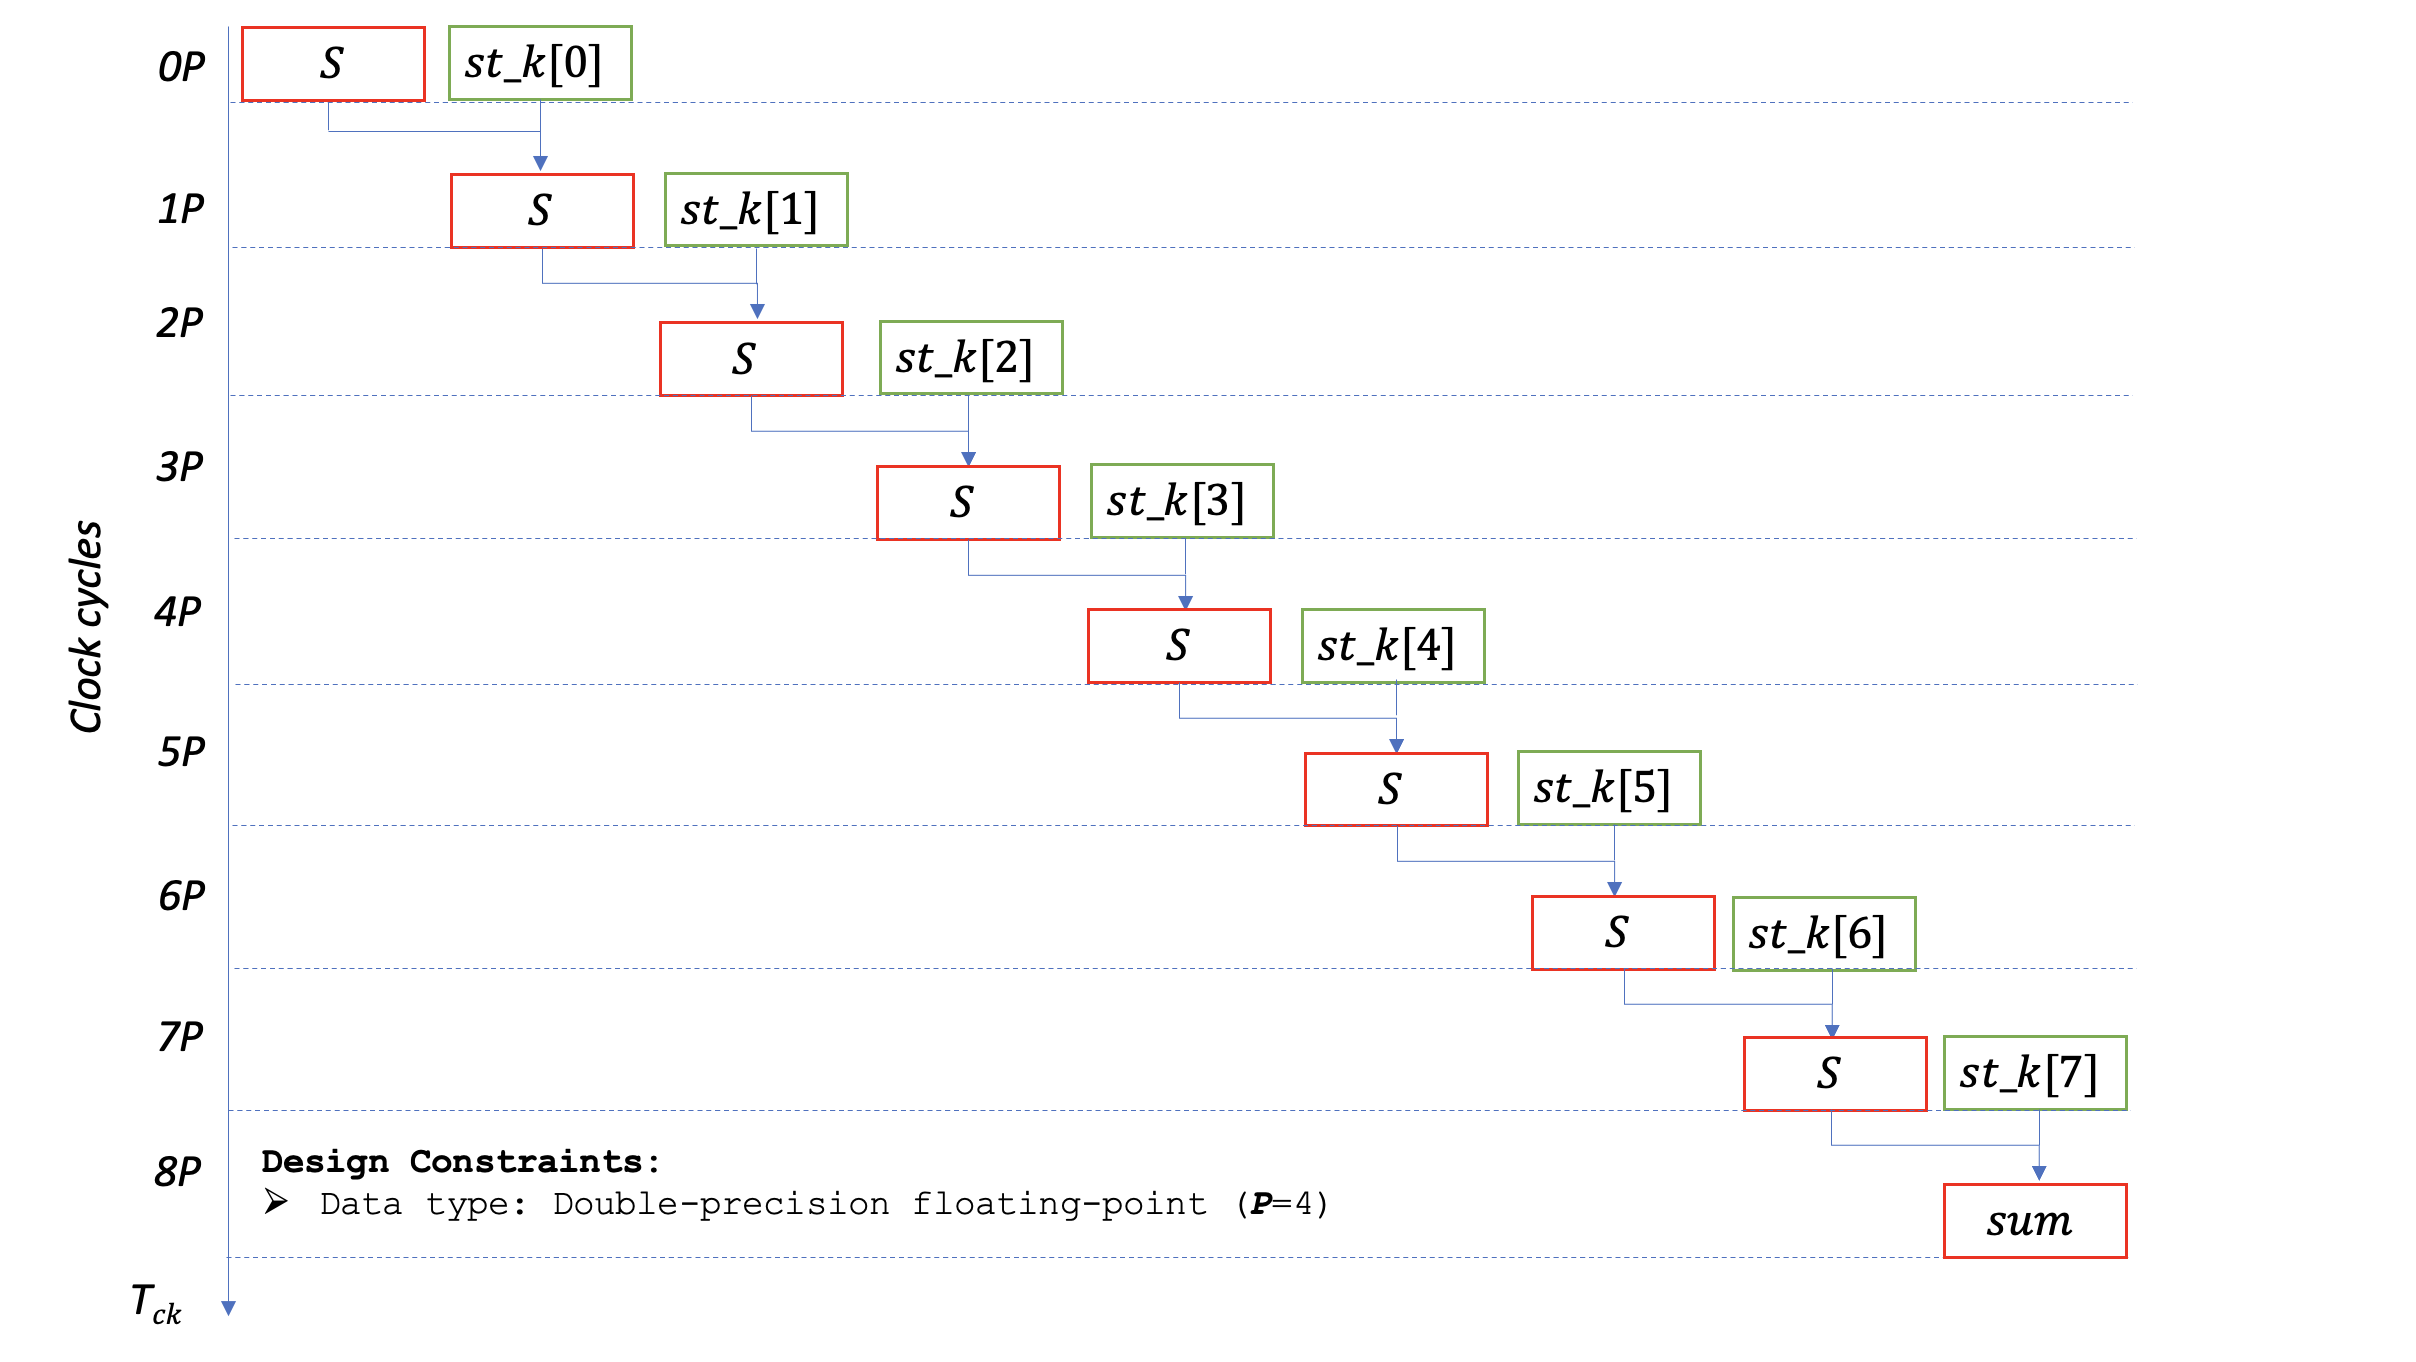
\includegraphics[width=0.8\textwidth]{\graphicsfolder/Figure1.png}
\end{center}
\label{fig:acc:baseline}
\small \textit{Note:} Data flow graph of a sequential accumulator circuit for adding double-precision floating-point elements of an array \texttt{st\_k} of size $\Naccsize=8$. The vertical dimension illustrates in which clock cycles these operations are performed (\textit{scheduling}). The circuit consists of one single double-precision floating-point adder, which performs an addition every $P>1$ clock cycles.
\end{figure}

While fully functional, the synthesized circuit is not efficient. Figure \ref{fig:acc:baseline} illustrates the associated data flow graph to clarify this point. The vertical axis denotes the passage of time in clock cycles, while the horizontal axis represents the circuits' functional units, consisting of additions and memory accesses in our example. The graph shows that every $P$ clock cycles, a new double-precision floating-point addition is performed. Accordingly, the synthesized circuit has a \texttt{for loop latency} of $\Naccsize\times P$ clock cycles: this is the time (measured in clock cycles) required for a circuit with a single physical adder to sequentially execute $\Naccsize=8$ additions (\texttt{loop iterations}) when each one of them takes $P> 1$ clock cycles (\texttt{iteration latency}).

We can enhance the efficiency of this circuit by reducing its \texttt{for loop latency}. The next sections introduce the main tools that economists can leverage in order to \textit{assist} the \texttt{HLS} compiler to design an effective \texttt{CL} design. We use the word assist deliberately. Unlike in the \texttt{RTL} approach, we do not design the circuit. Simply, we provide clues about acceleration opportunities that the compiler may not autonomously identify. 

We introduce these optimization techniques in an order that aligns with industry standards for hardware design optimization. Our overarching strategy is to initially establish an efficient circuit (Subsections \ref{sec:acc:fix-pre} and \ref{sec:acc:pipelining}) and subsequently enhance its performance by harnessing parallel computing opportunities (Subsection \ref{sec:acc:unroll}).

Throughout this process, we address potential bottlenecks that might hinder efficient design. This enables us to compile a list of critical hardware issues that economists are likely to encounter when accelerating their applications. Most importantly, it provides the core hardware design principles for accelerating economic models.

\subsection{Arbitrary-Precision Fixed-Point}\label{sec:acc:fix-pre}

We start our optimizations by targeting the \texttt{iteration latency}, $P$. This is the time required to execute the instructions in the body of the loop of Listing \ref{list:acc:seq} at any given iteration.  In our application, $P$ consists of the time necessary to perform two operations: reading an array element and accumulating it (see Figure \ref{fig:acc:baseline}). Here, we illustrate how we can reduce the execution time of the accumulation from multiple clock cycles to a single one by transitioning from single or double-precision floating-point data type (hereafter referred to as floating-point) to fixed-precision fixed-point (hereafter referred to as fixed-point) to represent the array elements.

Floating-point operations provide the IEEE754 standard for the finite precision approximation of real numbers. However, they cost hardware and energy and take multiple clock cycles to complete. In contrast, integer and fixed-point operations execute within a single clock cycle and, when properly implemented, deliver high accuracy.\footnote{See Appendix \ref{sec:flopre} for a brief overview of finite-precision fixed-point approximation.} Among others, \citet{yates2009fixed} provides guidelines for employing fixed-point arithmetic, and Subsection \ref{sec:pip} operationalizes them in our main application using \texttt{HLS} \citep{vitis-hls-ug1399}. 

Here, we illustrate how a few lines of code can recast floating- into fixed-point arrays by defining a type \texttt{fixed\_t} with the required precision in a header file, along with the necessary libraries.\footnote{This is one of the few optimizations that the \texttt{HLS} compiler cannot perform automatically since it requires users to specify the fixed precision parameters (72 and 21 in line 6). The macro \texttt{FIXED\_ACC} allows flexible toggling between double-precision floating-point and fixed-point for debugging purposes.}

\begin{lstlisting}[language=C,basicstyle=\footnotesize]
#define FIXED_ACC 1   
typedef double real;
#if FIXED_ACC
    #include <ap_int.h>
    #include <ap_fixed.h>
    typedef ap_fixed<72, 21> array_type;	
#else
    typedef real array_type;	
#endif
\end{lstlisting}

Conversely, the implementation of fixed-point arrays in \texttt{RTL} can be tedious even for experienced hardware designers. For example, the \texttt{RTL} designer must explicitly manage the proper alignment and interpretation of values with different fixed-point precision representations.

Besides reducing the iteration latency, recasting our operation in fixed-point also addresses two well-known bottlenecks that hinder the efficient design of an accumulation with addition operations: \textit{(i)} memory carry dependency; and \textit{(ii)} the lack of associativity property of floating-point additions. Subsection \ref{sec:acc:pipelining} demonstrates how fixed-point addresses the memory carry dependency problem, facilitating the creation of efficient pipelines. Subsection \ref{sec:acc:unroll} shows how properties of fixed-point arithmetic enable the implementation of a parallel reduce tree to solve our accumulation, further reducing the \texttt{for loop latency}.

\subsection{Pipelining and the Quest for an Initiation Interval of 1}\label{sec:acc:pipelining}

An ideal \texttt{CL} design keeps the circuit constantly busy (\textit{goal 1}) and starts new computations at every clock cycle (\textit{goal 2}). Here, we present an optimization tool that helps achieve both goals: hardware pipelining. In this context, we discuss how our solution of recasting our accumulator from floating- to fixed-point tackles a key obstacle to the efficient pipelining of our accumulation circuit: the memory carry dependency problem.

\subsubsection{Pipelining}

To understand hardware pipelining, we need to introduce the concept of \textit{initiation interval}, denoted as \textbf{II}. The \textbf{II} measures the number of clock cycles elapsed between the launch of two consecutive iterations in a loop. An ideal circuit has an $\textbf{II}=1$, and \textit{initiates} computations at every clock cycle. The following code listing uses the \texttt{\#pragma HLS pipeline II=1} directive to synthesize this design.

\begin{lstlisting}[language=C,caption= {Pipelined Accumulator},basicstyle=\footnotesize,label=list:acc:pip]
void hw_loop(array_type st_k[J],array_type &reduced_sum){
    array_type sum = 0.;
    for(int i=0;i<J;i++) {
        #pragma HLS pipeline II = 1
        sum+=st_k[i];
    }
    reduced_sum = sum;
    return;
}
\end{lstlisting}

To understand the hardware implications of this optimization technique, Figure \ref{fig:acc:fix:pip:seq:pip:pipfail} reports the data flows associated with four distinct hardware designs of our sequential accumulator: floating-point (Subsection \ref{sec:prohls}), fixed-point (Subsection \ref{sec:acc:fix-pre}), fixed-point with \textbf{II}=1, and floating-point with \textbf{II}=5. These graphs illustrate how the different \texttt{CL} designs engage their hardware components, often referred to as \texttt{pipeline stages}. They do so by reporting which data points each pipeline stage (horizontal axis) processes during each clock cycle (vertical axis). 

In the case of our sequential accumulator, the pipeline stages associated with the hardware implementation of the body loop's instructions (line 5 of Listing \ref{list:acc:pip}) consists of two operations: a reading and an accumulate operation. Later in our main application, these pipeline stages will consist of the hardware steps required to solve either the \textbf{IHP} problem in equation \eqref{eq:kopt} or the \textbf{Simulation} step.
 
The first two data flows on the left side of the figure illustrate how transitioning from floating- to fixed-point significantly reduces the execution time of the adder, from five to a single clock cycle, and, thus, the \texttt{iteration latency} from six to two clock cycles. Consequently, the total \texttt{for loop latency} drops from $P\cdot \Naccsize=6\cdot8=48$ clock cycles to $2\cdot8=16$ clock cycles. 
 
\begin{figure}[!htbp]
\caption{Data Flow of Sequential Accumulator with Pipelining}
\begin{center}
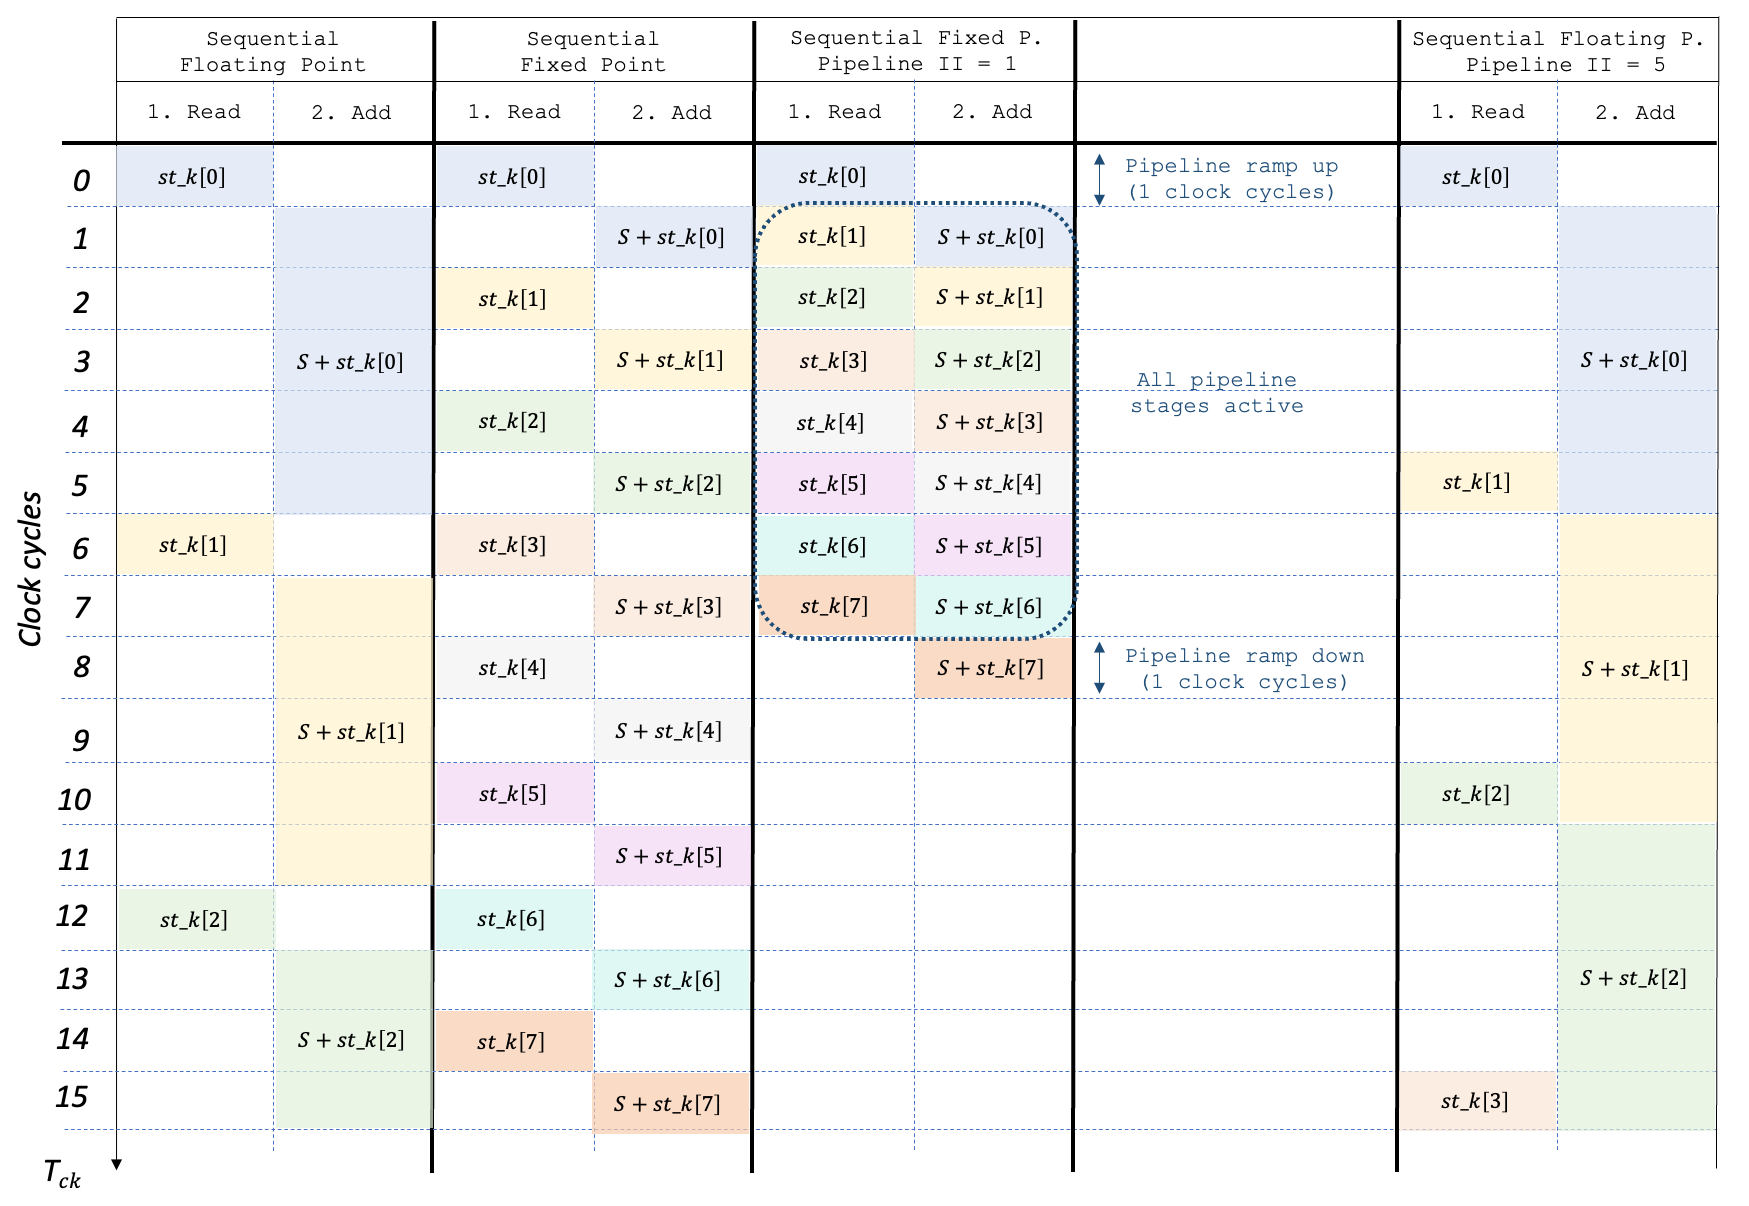
\includegraphics[width=\textwidth]{\graphicsfolder/Figure2.png}
\end{center}
\label{fig:acc:fix:pip:seq:pip:pipfail}
\small \textit{Note:} Data flow of four different hardware designs, from left to right: sequential floating-point (double precision), sequential fixed-point, sequential fixed-point pipeline with II=1, sequential floating-point (double precision) pipeline with \textbf{II} = 5.
\end{figure}

Listing \ref{list:acc:pip} improves over the sequential fixed-point design by instructing the \texttt{HLS} compiler to synthesize a fixed-point accumulator that initiates computations every clock cycle (\textbf{II}=1). This command generates a circuit that operates as follows. At clock cycle 0, the circuit starts reading \texttt{st\_k[0]} from memory. At clock cycle 1, the circuit initiates the first fixed-point addition $S=S+$\texttt{st\_k[0]}, while simultaneously loading \texttt{st\_k[1]} for a new accumulation. From clock cycle 1 to 7, the circuit reaches its maximum degree of \textit{instruction level parallelism}. At this point, all functional units of the circuit (\texttt{pipeline stages}) are working in parallel (attaining \textit{goal 1}), yielding an addition at every subsequent clock cycle (attaining \textit{goal 2}). The time required for all \texttt{pipeline stages} to become active is called pipeline \texttt{ramp up} and equals one clock cycle in our example. After clock cycle eight, the pipeline stages start to empty, as there are no more array elements to read. By clock cycle nine, all pipeline stages are empty. The time required to flush out the pipeline stages is called pipeline \texttt{ramp down}, also equal to one clock cycle in our application.  

As the state space increases, the pipeline ramp-up and ramp-down times become negligible with respect to the total for-loop latency. For example, when transitioning from an accumulation of an array of size 8 to an array of size 10,000 in equation \eqref{eq:Kagg}, the portion of \texttt{for loop latency} spent on filling and flushing the pipeline shrinks from 25\%, $\#\text{Stages}_{\text{ramp up+ramp down}}/J$=2/8, to a negligible 0.02\% (2/10000).

\noindent \textbf{Memory carry dependency problem.} Add-reduce accumulations inherently suffer from memory-carry dependencies because adding a new element of the array to the accumulation requires the previous element of the array to have already been incorporated (Figure \ref{fig:acc:baseline}). In the context of floating-point accumulations, this data dependency may impose a constraint on the lag (in cycles) at which new computations can be initiated (\textbf{II}).

For example, attempting to design a circuit with an \textbf{II}=1 would result in a synthesis failure, flagging a memory carry dependency violation. The reason becomes evident when inspecting the behavior of this circuit on the right-hand side of Figure \ref{fig:acc:fix:pip:seq:pip:pipfail}. The circuit must wait until clock cycle 5 for the value $S+st\_k[0]$ to become available before proceeding to the new addition $S+st\_k[1]$. Consequently, the best initiation interval for this design is every five clock cycles (\textbf{II}=5). Transitioning to fixed-point effectively addresses the memory dependency bottleneck by reducing the waiting time for the next element of the accumulation from five to just a single clock cycle, reaching \textbf{II}=1. 

\subsection{Loop Unrolling and Memory Management}\label{sec:acc:unroll}

So far, we have used \texttt{HLS} to design a circuit that efficiently initiates the necessary computations for a sequential accumulator at every clock cycle. Next, we further enhance its performance by introducing a powerful \texttt{HLS} tool that allows us to harness parallel computing opportunities: loop unrolling.
Alongside this, we address limitations associated with memory management and provide effective solutions. Furthermore, we discuss a common performance hurdle faced by the hardware implementation of an accumulator, such as equation \eqref{eq:Kagg}: the lack of associativity in floating-point additions. We conclude by explaining how our solution of recasting our accumulator from floating- to fixed-point effectively overcomes this challenge.

\subsubsection{Loop Unrolling}\label{sec:acc:loopunroll}

Our prior circuitry executed additions sequentially, overlooking the opportunity to exploit the data independence of array elements for concurrent parallel addition operations. In our accumulation example, and later in the acceleration of equation \eqref{eq:kopt} and Simulation step of the \citet{KrusellSmith1998} algorithm, we harness this parallelism by deploying the \texttt{\#pragma HLS unroll factor = X}. This directive creates multiple physical replicas (\texttt{X}) of the circuit described within the loop's body (line 6 of Listing \ref{list:acc:unroll:arr:part}) and \textit{autonomously} organizes them to operate in parallel in a reduce-tree pipeline, which we will describe momentarily. Intuitively, the more physical replicas operating in parallel (\texttt{unroll factor}), the fewer iterations are necessary to perform the final accumulation, lowering the \texttt{for loop latency}. The following listing synthesizes a pipeline that processes in parallel all elements of the array, $\Naccsize=\texttt{unroll factor}=8$.

\begin{lstlisting}[language=C,caption= {Accumulator with Loop Unrolling of Factor 8},basicstyle=\footnotesize,label=list:acc:unroll:arr:part]
void hw_loop(array_type st_k[J],array_type &reduced_sum){
    #pragma HLS array_partition variable = st_k factor = 4 type = cyclic	
    array_type sum = 0.;
    for(int i=0;i<J;i++) {
        #pragma HLS unroll factor=8
        #pragma HLS pipeline II = 1
        sum+=st_k[i];
    }
    reduced_sum = sum;
    return;
}
\end{lstlisting}

\noindent \textbf{Associative reduce tree and fixed-size loop bounds.} Figure \ref{fig:acc:fix:unroll8:bram} shows that an unroll factor of 8 prompts the compiler to \textit{autonomously} generate an associative reduce tree structure with a \texttt{pipeline depth} of three layers, resulting in an accumulation every three clock cycles.\footnote{In the first clock cycle, the compiler simultaneously reads all elements of the array. In the second clock cycle, it performs four additions in parallel. In the third clock cycle, it performs two additions and reduces the accumulation to a final digest. The fourth clock cycle appears when $\Naccsize>\texttt{unroll\_factor}$, in which case the accumulation of 8 elements is added to the overall rolling sum. See Appendix \ref{app:ass:red:tree} for more details.} This design is facilitated by the fact that the loop bounds are fixed (0 and $\Naccsize$), and increments of the loop iterator $i$ are constant (and equal to 1). These clues allow the compiler to aptly determine the required number of layers: $O(\ln_{2} \texttt{unroll factor})$.

\begin{figure}[ht!]
\caption{Data Flow of Accumulator with Loop Unroll}
\begin{center}
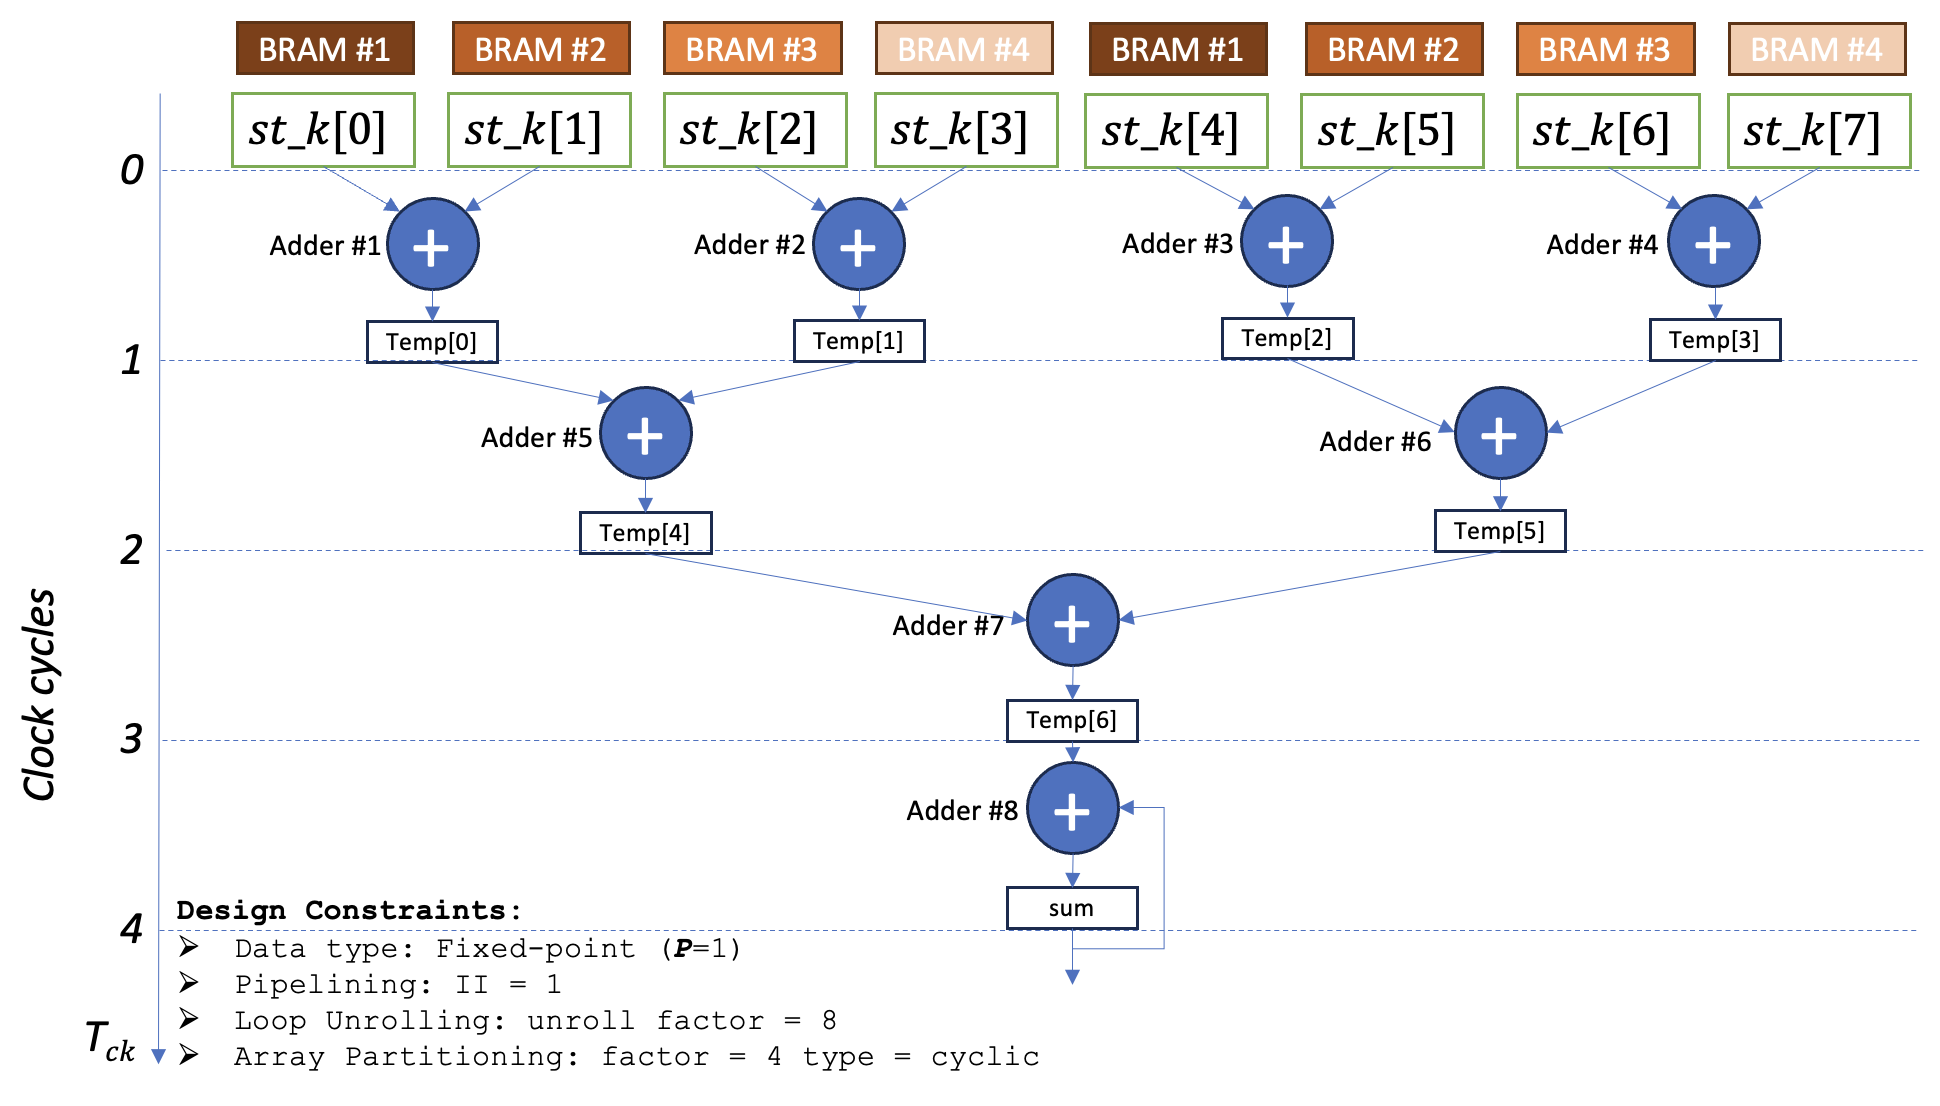
\includegraphics[width=1\textwidth]{\graphicsfolder/Figure3.png}
\end{center}
\label{fig:acc:fix:unroll8:bram}
\small \textit{Note:} Data flow graph of a circuit that unrolls by a factor of 8 the addition of the fixed-point elements of an array \texttt{st\_k} of size $\Naccsize=8$. The vertical dimension illustrates in which clock cycles these operations are performed (\textit{scheduling}). The circuit consists of eight fixed-point adders, which perform an addition every clock cycle. \texttt{BRAM \#1-\#4} denote four local memories used to partition the \texttt{st\_k} array. 
\end{figure}

When the array of size $\Naccsize$ is larger than the \texttt{unroll factor}, this circuit produces an accumulation every $\Naccsize/\texttt{unroll}$ $\texttt{factor} + \ln_2(\texttt{unroll\_fac}\texttt{tor}) + 1$ clock cycle. The first term illustrates how loop unrolling decreases the \texttt{for loop latency} from  $\Naccsize$ to $\Naccsize/\texttt{unroll factor}$ by placing enough hardware, as determined by \texttt{unroll factor}. The second term captures the pipeline ramp-up time.\footnote{The third term appears when $\Naccsize>\texttt{unroll factor}$ and captures the time required to incorporate the result of the reduce tree into the rolling accumulation (clock cycle 4 in Figure \ref{fig:acc:fix:unroll8:bram}). Otherwise, the term disappears.} As discussed in Subsection \ref{sec:acc:pipelining}, the pipelining performance of this circuit increases with the size of the state space. As $\Naccsize$ increases, the pipeline ramp-up time becomes negligible with respect to the total accumulation time, which converges to $\Naccsize/\texttt{unroll factor}$. 

While the acceleration achieved with loop unrolling resembles the single instruction, multiple data acceleration exploited by GPUs, it differs in important dimensions. First, the \texttt{HLS} compiler designs new hardware with the requested level of parallelism, whereas GPUs exploit existing one. Consequently, while GPUs may experience performance degradation when the required level of parallelism does not effectively engage all their cores (\citealp{Aldrich2011}), FPGAs are affected to a much lesser extent. Second, FPGAs allow the implementation of hardware designs of intricate algorithms, whereby various facets of the application can exploit different acceleration strategies. The \citet{KrusellSmith1998} algorithm exemplifies this complexity, transitioning from a policy function iteration algorithm that benefits from reduced evaluation latency through instruction-level parallelism and pipelining (Subsection \ref{sec:acc:pipelining}) to a multi-parameter exploration or multiple-actor simulation step, which benefits from data-level parallelism. While GPUs thrive in the latter, they cannot reduce evaluation latency.

To conclude, note the \texttt{\#pragma HLS array\_partition} directive at line 2 of Listing \ref{list:acc:unroll:arr:part}. Next, we discuss how this command addresses a potential issue related to memory management that \emph{may} prevent \texttt{HLS} from synthesizing the required circuit. 

\subsubsection{Memory Management}\label{sec:memman}

Now, we discuss two main limitations regarding memory management: large memory access latency and array partitioning.

\noindent\textbf{Large memory access latency.} The FPGA device and host processor share a common memory referred to as global memory (dynamic random access memory, DRAM). Global memory is large (tens of gigabytes) and, thus, useful for storing input, intermediate, and output data. In our accumulator design, we initialize our array in double-precision floating-point in the host processor, \texttt{st\_in}, and make it available to the FPGAs by storing it in global memory. Access to this memory is slow (hundreds of clock cycles). 

To solve this problem, we can copy chunks of data from the large global memories to on-chip local memories, which are small but numerous and can be accessed in a single clock cycle: block RAMs (BRAMs), ultraRAMs (URAM), LUT RAMs, registers. The following listing illustrates how straightforward it is to copy the array from global (\texttt{st\_in}) to local memories (\texttt{st\_k}) through the implementation of a simple array assignment.

\begin{lstlisting}[language=C,caption=Store Data from Global to Local Memories,basicstyle=\footnotesize, label=lis:init:k]
void hw_top_init(real *k_in, array_type st_k[J]){
    init_1:
    for (int i = 0; i < J; ++i)
        st_k[i] = (array_type) k_in[i];
    return;
}
\end{lstlisting}

Note the type cast operation that converts the floating-point values of the array initialized by the host, \texttt{st\_in}, into the fixed-point array declared in the local memories, \texttt{st\_k}. Without loss of generality, we assume that \texttt{st\_k} has been stored in BRAMs in all our designs.

\noindent\textbf{Array partitioning.} When transferring data from global to local memory, compilers optimize on-chip resource use by storing contiguous elements of \texttt{st\_k} in the same BRAM before moving on to the next. For instance, without further instructions, Listing \ref{lis:init:k} stores all the elements of \texttt{st\_in} in a single BRAM, which, without loss of generality, we refer to as \texttt{BRAM \#1}.

Each BRAM provides two read-write ports, allowing for a maximum of two concurrent read-write operations.
Accordingly, while resource-efficient, this storage scheme can lead to a memory bottleneck when the total number of required reads from multiple pipelines (determined by the \texttt{unroll factor} multiplied by the simultaneous reads per pipeline) surpasses the available reading ports per shared BRAM.

The memory-access bottleneck becomes evident in our example when we instruct the compiler to synthesize four physical adders in parallel (Listing \ref{list:acc:unroll:arr:part}). In this scenario, during the first clock cycle, we can only read a maximum of two out of the eight \texttt{st\_k} values stored in the single BRAM. Consequently, the synthesis process fails to produce the required \texttt{CL} design. Instead, it results in a circuit with an accumulation process that resembles the sequential addition described in Subsection \ref{sec:acc:pipelining} (see also Figure \ref{fig:acc:fix:unroll8:fail} in Appendix \ref{sec:membot}).

The memory bottleneck can be resolved by strategically distributing the elements of \texttt{st\_k} across multiple BRAMs to accommodate the eight memory accesses required by the four parallel pipelines.
The achieve this, we use the \texttt{\#pragma HLS array\_partition} directive at line 2 of Listing \ref{list:acc:unroll:arr:part}. This directive employs a \texttt{cyclic} array partitioning with a 
\texttt{factor} of 4 to interleave the elements of \texttt{st\_k} across \texttt{BRAM \#1-\#4}, as depicted in Figure \ref{fig:acc:fix:unroll8:bram}.\footnote{Cyclical array partitioning creates \texttt{factor = 4} smaller arrays from \texttt{st\_k} by copying elements cyclically, and storing them in independent BRAMs. For instance, \texttt{st\_k[0]} goes into \texttt{BRAM \#1}, \texttt{st\_k[1]} into \texttt{BRAM \#2}, \texttt{st\_k[2]} into \texttt{BRAM \#3}, \texttt{st\_k[3]} into \texttt{BRAM \#4}, \texttt{st\_k[4]} into \texttt{BRAM \#1} and so on until completion. For a discussion of the different array partitioning types (cyclic, block, and complete), we refer to \url{https://docs.xilinx.com/r/en-US/ug1399-vitis-hls/pragma-HLS-array_partition}.}

\noindent\textbf{Automatic optimizations.} We explain here the emphasis on the word \textit{may} at the end of Subsection \ref{sec:acc:unroll}. In our simple accumulator example, for a given \texttt{unroll factor}, the \texttt{HLS} compiler recognized the need to partition the array \texttt{st\_k} without explicit clues from the array partitioning \texttt{\#pragma}. As compiler technology evolves, we anticipate such automation to expand to even more intricate circuits. Our performance analysis of the \citet{KrusellSmith1998} algorithm in Section \ref{sec:acc} demonstrates the advanced nature of these automations already in place.

\subsubsection{Non-Associativity of Floating-Point Addition} 

Here, we discuss how using floating-point additions prevents the compiler from autonomously generating the associative reduce tree displayed in Figure \ref{fig:acc:fix:unroll8:bram}. Computers carry out computation on numbers with finite representations. When we abandon the field of real numbers $(\mathbb{R},+,\times,\geq)$ for their IEEE754 floating-point, finite-precision approximation, we lose the associative property of the addition. \citet{Goldberg1991} provides an example by showing how $(x + y) +z$ and $x + (y +z)$ give different results when $x = 1e30$, $y = -1e30$ and $z = 1$. The first equals 1, and the second equals 0 (since $y+z$ rounds to $-1e30$ before performing the addition with $x$). Accordingly, compilers have historically been prevented from rearranging floating-point additions (like in Figure \ref{fig:acc:fix:unroll8:bram}) in order to avoid producing a different result than the original code. This rule downplays the fact that the source code may have been written in a loop simply for convenience, without a specific order of additions in mind. As a result, the compiler still insists on performing the floating-point sum sequentially in $\Naccsize\cdot P$ cycles, as shown in Figure~\ref{fig:acc:baseline}, even if we allowed it to use more hardware.

In our accumulator example (later deployed in the \citealp{KrusellSmith1998}, application), we tackle this issue by performing the accumulation in fixed-point, where the associative property still holds, and the compiler knows it is safe to re-associate the additions since the computed result will be the same. For alternative strategies to handle this issue while maintaining floating-point, we refer to \cite{hrica2012floating} and \cite{kadric2016accurate}. In contrast to these strategies, our fixed-point approach (Subsection \ref{sec:acc:fix-pre}) also addresses the long latency of floating-point additions with minimal compromises in accuracy, as demonstrated by our application.

\subsection{Portability, Code Reusability, and Programming Languages}

\texttt{C}-code designed for FPGA acceleration using \texttt{HLS} exhibits remarkable portability. As our accumulation example demonstrates, the code compiles and runs on CPUs (including vector and SIMD computations) without modifications. Non-FPGA compilers ignore the \texttt{HLS \#pragma}s, eliminating the need to maintain a separate codebase for FPGA acceleration. 

Furthermore, high-level computational components, such as accumulation (discussed here), interpolation, and simulation (discussed later), are common in economic models. Much like economists use function libraries to address recurring algorithms, the same \texttt{HLS}-enhanced codes and associated hardware components can be repurposed to accelerate recurring aspects of different models. 

While \texttt{HLS}-enhanced \texttt{C}-code is highly portable, FPGA platform-specific optimizations and design may still require special considerations. First, fine-tuning an application for a specific FPGA involves adjusting parameters like loop unrolling or array partitioning, considering both application-specific and platform-specific factors, such as the execution frequency of particular portions of code and their resource utilization. These refinements only require changes to specific arguments in the \texttt{\#pragma}s, leaving the base \texttt{C}-code unchanged. Recent advancements in automatic compilation and optimization hold great promise for automating these optimizations with solvers and autotuners (as discussed below), removing the need for manual changes by the developer.\footnote{We can determine these tuning parameters as the ones that maximize performance while staying within the constraints of available FPGA hardware resources. Solvers or autotuners can then automate the selection of these values, streamlining the optimization process (\citealp{atlas_ics1998,spice_fpl2009,model_based_hls_fpl2016,comba_trcad2020}).} Second, interfacing with platform-specific components, like memory interfaces and I/O ports, super logic regions (SLRs) may be necessary for advanced designs (see Subsection \ref{sec:cusloghardes}). To mitigate these platform-specific concerns, we showcase FPGA acceleration on \texttt{AWS}, a cloud-based service that offers widespread access to \textit{identical} high-performance FPGA devices. In addition, our tutorial provides \textit{all} the necessary boilerplate code to harness these platform-specific components.

To conclude, recent years have seen great advances in the incorporation of hardware design tools among popular programming languages, like \texttt{Python}, \texttt{Julia}, and \texttt{Matlab} (e.g., \citealp{quenon2021towards}, \citealp{biggs2022high}). Our accumulator best exemplifies these efforts. The \texttt{Matlab} suite has incorporated an \texttt{HDL} coder that generates the \texttt{RTL} code of a variety of functionalities, including the accumulator we just described in this section.\footnote{See \url{https://www.mathworks.com/help/fixedpoint/ref/sum.html}.}  Overall, high-level synthesis compilers are bound to become more popular among high-level software languages, further easing economists' access to custom accelerators.

\section{Our Application}\label{sec:accschhar}

This section illustrates how we deploy the FPGAs' optimization tools introduced in our previous section to accelerate the \citet{KrusellSmith1998} algorithm in Section \ref{sec:alg}. We present the FPGA acceleration approach in Subsection \ref{sec:fpgaacc} and the CPU counterpart in Section \ref{sec:cpuacc}. Appendix \ref{sec:aws:tecspe} reports the hardware specifications of the different \texttt{AWS} instances.

\subsection{Hardware Architecture of FPGA Acceleration}\label{sec:fpgaacc}

The FPGA acceleration approach solves the \citet{KrusellSmith1998} algorithm as implemented by \cite{MaliarMaliarValli2010} in Section \ref{sec:alg} by using Amazon F1 instances to deploy three configurations of FPGAs connected to a host: one FPGA (\awsinstfI), two FPGAs (\awsinstfII), and eight FPGAs (\awsinstfIII). 

The computational flow is as follows. The host initializes variables (grids, shocks, guesses), allocates jobs across available FPGA(s), and transfers the data to the FPGA(s). The FPGA(s) then execute(s) the \textit{kernel}: the nested, fixed-point algorithm detailed in Section \ref{sec:alg}. Subsequently, the host reads back and saves the results. Unless differently specified, computations employ the IEEE754 double-precision floating-point format. 

\subsubsection{FPGA Hardware Description}\label{sec:FPGAhardes}

F1 instances mount (up to eight) Xilinx VU9P FPGAs, each with 1.2 million 6-input gates (LUTs), 6,840 multiply-accumulate units (DSPs), and 346Mb of on-chip memory, given by 76Mb of block RAM (BRAM) and 270Mb of ultra RAM (URAM). These resources are organized in three dies, referred to as a SLR, connected by a silicon interposer (see Figure \ref{fig:threekernel}). The AWS FPGA is further divided into two partitions: shell and custom logic (\texttt{CL}). The shell is the FPGA platform implementing external peripherals, such as peripheral component interconnect express (PCIe) and dynamic random access memory (DRAM). Users' \texttt{CL} designs can employ up to \CLdesignLUT\, LUTs, \CLdesignDSP\, DSPs, and \CLdesignonchipmemory\, of on-chip memory, given by \CLdesignBRAMMemory\, of BRAM and \CLdesignURAMMemory\, of URAM per FPGA.

\subsubsection{Custom Logic Hardware Design}\label{sec:cusloghardes}

Now, we operationalize the FPGA optimization tools discussed in Section \ref{sec:buiblo} to accelerate the \cite{KrusellSmith1998} algorithm. In addition, we show how our \texttt{CL} design exploits platform-specific characteristics of the F1 instances' FPGAs: the presence of three SLRs. As mentioned above, the Xilinx VU9P FPGAs are organized in three dies, whose custom logic can be jointly or independently used for acceleration purposes. For our application, we tailor our \texttt{CL} design to compute three economies in parallel, one per SLR, in the same FPGA.\footnote{We could alternatively design the \texttt{CL} to span across the multiple SLRs. This design would require handling inter-SLR connections, complicating the coding, and the management of tighter clock constraints. Since many of the benefits of accelerators are associated with the estimation of structural parameters that involve the computation of several thousand economies (each associated with a different set of parameter values), our hardware design is appropriate. The single SLR solution is still \fpgaspeedIknlICPUI times faster than the sequential execution in the CPU (Subsection \ref{sec:rob}).}

\citet{FPGAtutorial23} describe in detail how the \texttt{OpenCL} commands organize the computation flow in kernels. Each kernel is assigned a different economy $\underline{\theta}$ and is instantiated in a separate SLR. Kernels are then deployed in parallel. A feature of this hardware design is that it is easily scalable with minimal modifications of the \texttt{C/C++} code. \texttt{OpenCL} commands collect the available SLRs and instantiate the kernels. In the case of one FPGA (\awsinstfI), three kernels are instantiated across the available SLRs. In the case of eight FPGAs (\awsinstfIII), 24 kernels are launched in parallel.

To load and deploy our custom logic hardware design on the EC2 F1 instances, we create Amazon FPGA Images (AFI) that combine the shell and the \texttt{CL} design for multiple grid sizes. We accomplish this step by creating.AWSXCLBIN files.

\subsubsection{The Single-Kernel Design}\label{sec:kerdes}

Our kernel implements in hardware the nested-fixed-point algorithm presented in Section \ref{sec:alg}. The design organizes the three inter-dependent building blocks --IHP, simulation, and ALM-- in a sequence, and it performs the computations until convergence of the ALM coefficients in equation \eqref{eq:betaconv}.

Following Amdahl's law, our \texttt{CL} design allocates hardware resources to balance the time spent on the two time-consuming steps of the algorithm: the \textbf{IHP} and Simulation design. Our final kernel design starts computations at every clock cycle at 250 MHz and provides flexibility to study multiple grid sizes. 

To reach an \textbf{II} of 1, we address the challenges discussed in Section \ref{sec:buiblo} as follows. First, we tackle the two memory management bottlenecks: \textit{(i)} large memory access latency; and \textit{(ii)} limited memory ports to access data in parallel. We fix the first issue by copying data in local memories that can be accessed in a single clock cycle. Our FPGA has enough local memories to store all of the input data for our application (Table \ref{tab:res}). Hence, we need to transfer the input data only once per kernel computation. We address the second issue by deploying the array partitioning \texttt{\#pragma} to store multiple copies of the same data in as many independent local memories as required by the number of pipelines performed in parallel.

Next, we turn to application-specific interventions essential for achieving an \textbf{II} of 1, specifically the acceleration of the linear interpolation within the \textbf{IHP} and \textbf{Simulation} steps. A well-known computational challenge in interpolation is to find the interval of interpolation. We accelerate this step by implementing an efficiently pipelined (\textbf{II} of 1) jump search algorithm with fixed-size loop bounds.\footnote{As discussed in Subsection \ref{sec:acc:loopunroll}, the presence of \textit{fixed} interpolation grids' bound allows the compiler to autonomously determine the depth of the reduce tree required to find the interpolation interval.} To ensure that the algorithm does not introduce any unwanted bias, we verify that it outperforms alternative search algorithms in the CPU (Table \ref{tab:CPUben}).

\textbf{The individual household problem (IHP) design.} The \textbf{IHP} design implements the previous steps to reach an \textbf{II} of 1 in equation \eqref{eq:kopt} by pipelining the operations involved in the computation of the expectation as discussed in Subsection \ref{sec:acc:pipelining}. We further accelerate the design by using the partial loop unrolling technique discussed before to place two pipelines to work in parallel on the (sequential) solution of equation \eqref{eq:kopt} at different states $\{\state\}$ (more pipelines are hard given the hardware limits). Given the current guess of individual capital holdings, the IHP design solves equation \eqref{eq:kopt} for every state and updates the guess according to equation \eqref{eq:kupdate}, as discussed in Subsection \ref{sec:alg}.B.\textit{(ii)}. These steps are iterated until convergence, as per equation \eqref{eq:ktoll}. 

\textbf{The simulation design.} The simulation design in Subsection \ref{sec:alg}.D.\textit{(ii)}.\textit{(b)} is divided into two steps, each accelerated with a custom pipeline. The first step is represented by the accumulation operation required to compute the cross-sectional average of the individual household's capital holdings, $m_{t}$, in equation \eqref{eq:Kagg}. To achieve an $\textbf{II}=1$ at this step, we deploy the custom pipelined fixed-point accumulation operator discussed in Section \ref{sec:buiblo}. Indeed, the best acceleration performance for our benchmark model is reached by letting the compiler perform automatic optimizations. The second step is represented by the interpolation step involved in the computation of next-period household capital holdings. We reach an $\textbf{II}=1$ by implementing the aforementioned jump search algorithm.\footnote{To achieve an $\textbf{II}=1$ in both steps, we create multiple copies of the input data to avoid memory access bottlenecks. The simulation requires a large number of individual shocks ($10,000\times1,100$). To minimize the memory usage, we encode the $\{0,1\}$ shocks (from integers) into bits and pack them in groups of eight into a single byte of memory (8 bits) in both the FPGA and the CPU. Further, we tell the compiler to store these shocks in the URAMs, which have wide arrays of 72 bits and allow us to store 64 shocks (of size 1 bit) in each of these arrays. By doing so, we need to access the memory only once every 64 iterations.}

\textbf{The ALM design.} The ALM step involves several resource-expensive operations but has very small latency (\ALMtimebaseline).\footnote{The ALM step requires \ALMresourcesexplog.} Accordingly, we provide instructions to the compiler to not perform any pipeline or unrolling and further instruct it to limit the number of hardware resources used.

\subsubsection{The Three-Kernel Design}\label{sec:kerdesthree}

Our \texttt{CL} design is tailored to compute three economies in parallel by exploiting the three hardware regions available for hardware design: the SLRs. To reach this goal, we modify our single-kernel design to handle the resource limitations. Our single-kernel design barely fits in one of the SLRs, slightly leaking into one of the adjacent SLRs with non-time-critical operations (Figure \ref{fig:singlekernel}). The Amazon shell --which provides useful hardware resources to facilitate the \texttt{HLS} kernel design-- exacerbates this problem by consuming part of the resources in two of the three adjacent SLRs. To fit the three kernels, we provide directives that limit the degree of partial unrolling in the IHP. The resulting three-kernel design (Figure \ref{fig:threekernel}) trades off the single-kernel performance for the parallel execution speedup.

\subsection{Hardware Architecture of CPU Multi-Core Acceleration}\label{sec:cpuacc}

The CPU multi-core acceleration approach solves our model using Amazon M5N instances by parallelizing data-independent tasks (economies) across multiple physical cores: one core (\cpuI), eight cores (\cpuII), and forty-eight cores (\cpuIII). Appendix \ref{sec:aws:tecspe} justifies the choice of these instances.

Our benchmark CPU kernel is an optimized \texttt{C++}-version of the original \citet{MaliarMaliarValli2010} \texttt{Matlab} code, whose sequential single-core solution of the baseline economy is \speedCvsMatlab\, as fast as the original \texttt{Matlab} code, an expected speedup given the results in \citet{Aruoba2015}. The CPU kernel utilizes a jump search algorithm in order to determine the interpolation interval over the individual capital holdings grid. Table \ref{tab:CPUben} shows that this algorithm outperforms standard alternatives in the CPU, ensuring the best CPU kernel performance.

\begin{table}[ht!]
\caption{Benchmarking the CPU: Alternative Search Algorithms}
\vspace{-0.1in}
\begin{center}
\setlength\tabcolsep{4pt}
\begin{tabular}{@{\extracolsep{\fill}}lccccccc}
\toprule
&\multicolumn{1}{c}{\textbf{Linear Search}}&
&\multicolumn{1}{c}{\textbf{Binary Search}}&
&\multicolumn{1}{c}{\textbf{Jump Search}}\\
\textit{Solution Time} &\cpulineartime &&\cpubinarytime &&\cpujumpsearchtime\\
\textit{Speedup} & - &&\cpubinaryspeedup &&\cpujumpsearchspeedup\\ 
\bottomrule
\end{tabular}
\label{tab:CPUben}
\end{center}
\small \textit{Note:} 
Solution time (in seconds) and speedups of alternative interpolation interval search algorithms. Speedups are computed relative to the linear search algorithm. Results are obtained by solving \numbeconII baseline economies sequentially using a single core instance (\cpuI).
\end{table}

We operationalize the multi-core parallelization by using the open source message passing interface (\texttt{Open MPI}).\footnote{See \href{https://www.open-mpi.org}{https://www.open-mpi.org}. We use \texttt{Open MPI: Version 4.1.1.}} \texttt{Open MPI} provides easily implementable, off-the-shelf routines for parallelizing data-independent tasks across multiple cores. In contrast with alternative multi-core parallelization (like \texttt{OpenMP}), \texttt{Open MPI} does not require different cores to share the same memory. This feature makes \texttt{Open MPI} particularly appealing for massive data parallelization, from small clusters up to medium/large-scale supercomputers.

Our computational flow is as follows. \texttt{Open MPI} routines determine the number of cores available and uniformly spread the number of (data-independent) economies to be computed across the different cores. For example, the solution of \numbeconII economies on a 48-core machine would have \texttt{Open MPI} allocating 25 economies per core. Each core will then independently complete the assigned tasks. 

\section{Quantitative Results}\label{sec:quantitative}

We assess the efficiency gains of FPGA acceleration against CPU cores by measuring efficiency gains in solution speedup, AWS costs, and energy savings. We choose as a benchmark the CPU rather than the graphic processing units (GPUs) for two reasons. First, CPUs are still more commonly used in economics than GPUs, making the interpretation of our results more transparent. Second, differently from the CPU, the effectiveness of GPU acceleration is heavily dependent on software optimizations (e.g., memory management), making the benchmark performance more susceptible to software engineers' choices. Nonetheless, for completeness, we implement the \cite{MaliarMaliarValli2010} algorithm in \texttt{python/1.13} and accelerate it using the \texttt{Numba Cuda compiler} on an \texttt{NVIDIA A100} GPU. Consistent with the finding in \cite{Aldrich2011} for GPU acceleration on small grids, the GPU is ``only'' \speedGPUvsMatlab\ as fast as the original \texttt{Matlab} code. While the implementation of the algorithm with \texttt{C-cuda} and additional memory optimizations might yield further speedups, it is most unlikely that GPUs can deliver the same performance as the FPGA for this particular application.

To make our acceleration comparison as meaningful as possible, we proceed as follows. First, our FPGA and CPU kernel share the same \texttt{C/C++} code to solve the same algorithm in both platforms. Hence, the observed speedup is the result of a margin available to the electrical engineer economist (designing hardware) and not to the software engineer economist (writing better code for CPUs and GPUs). 
Using the optimization techniques discussed in Section \ref{sec:buiblo}, we program the logic of our FPGA to accelerate the \cite{KrusellSmith1998} algorithm. In comparison, the CPU and GPU logic cannot be programmed. The CPU is premanufactured to optimize the performance of sequential instructions needed in daily computer activities, which include not only simulating our models but also browsing the internet, checking emails, and so forth. As such, it lacks the gains from hardware specialization that are accessible to FPGAs. That said, the \texttt{C++}-compiler on a CPU and GPU goes a long way to execute the code as fast as possible by \textit{automatically} performing low-level instruction parallelism. We can instruct the compiler to do this as much as possible by compiling the code using the aggressive \texttt{-03} optimization flag in our \texttt{G++} compiler.

Second, our baseline comparison is that of a single FPGA chip against a single CPU core while computing $N_{E}$ economies (which we will define momentarily). This benchmark provides an apple-to-apple comparison of the differential performance of the two accelerators.

Third, we introduce a multi-economy parallelism to get insights into the potential of FPGAs to structurally estimate our model by solving it for many different parameter values. But we do so in a controlled way. A well-known drawback of \texttt{Open MPI} parallelization is that the total execution time is determined by the execution time of the slowest core. To temper this effect, first, we pick a number of economies ($N_{E}=$\numbeconII) that is uniformly divisible across the different CPU cores in our AWS instances (1, 8, 48 cores). Second, we determine the benchmark speedup (Table \ref{tab:baseline}) by solving the same economy (i.e., the same set of parameter values) multiple times. In this way, we eliminate heterogeneity in the solution time attributed to differences in convergence of the iterative algorithm with different parameter values. Under this setup, we ensure that we use all CPU cores and that the speedup scales linearly with the number of cores. Incidentally, this exercise illustrates how easy it is to implement increasingly aggressive acceleration by deploying multiple FPGAs in parallel, a dimension not explored in \cite{Peri2020}.

In summary, our benchmarking strategy eliminates all differences in performance between FPGAs and CPUs that are not inherently linked to the differences in their architecture. If we could rewrite the solution algorithm more efficiently, that better code would improve the performance of both FPGAs and CPUs and leave the relative performance (roughly) unchanged.

\begin{table}[ht!]
\caption{Efficiency Gains and Implementation Costs of FPGA Acceleration}
\label{tab:baseline}
\vspace{-0.1in}
\begin{center}
\begin{subtable}{\textwidth}
\caption{Efficiency Gains of FPGA Acceleration}
\label{tab:baseline:A}
\setlength\tabcolsep{4pt}
\begin{tabularx}{\textwidth}{XXXXXXXXXXXXX}
\toprule
&&\multicolumn{3}{c}{\textbf{Speedup}}&&\multicolumn{3}{c}{\textbf{Relative Costs (\%)}}&&\multicolumn{3}{c}{\textbf{Energy (\%)}}\\
\cmidrule{3-5} \cmidrule{7-9} \cmidrule{11-13}
\multirow{2}{*}{\textit{CPU-cores}}        &&\multicolumn{3}{c}{\textit{FPGAs}}&&\multicolumn{3}{c}{\textit{FPGAs}}&&\multicolumn{3}{c}{\textit{FPGAs}}\\
&&\multicolumn{1}{c}{\textit{1}}&\multicolumn{1}{c}{\textit{2}}&\multicolumn{1}{c}{\textit{8}}&&\multicolumn{1}{c}{\textit{1}}&\multicolumn{1}{c}{\textit{2}}&\multicolumn{1}{c}{\textit{8}}&&\multicolumn{1}{c}{\textit{1}}&\multicolumn{1}{c}{\textit{2}}&\multicolumn{1}{c}{\textit{8}}\\
\cmidrule{3-5} \cmidrule{7-9} \cmidrule{11-13}        
\textit{1}&&\fpgaspeedICPUI&\fpgaspeedIICPUI&\fpgaspeedIIICPUI&& \fpgacostICPUI&\fpgacostIICPUI&\fpgacostIIICPUI&& \fpgaenergyICPUI&\fpgaenergyIICPUI&\fpgaenergyIIICPUI \\
\textit{8}&&\fpgaspeedICPUII&\fpgaspeedIICPUII&\fpgaspeedIIICPUII&&\fpgacostICPUII&\fpgacostIICPUII&\fpgacostIIICPUII&&\fpgaenergyICPUII&\fpgaenergyIICPUII&\fpgaenergyIIICPUII \\
\textit{48}&&\fpgaspeedICPUIII&\fpgaspeedIICPUIII&\fpgaspeedIIICPUIII&&\fpgacostICPUIII&\fpgacostIICPUIII&\fpgacostIIICPUIII&&\fpgaenergyICPUIII&\fpgaenergyIICPUIII&\fpgaenergyIIICPUIII \\
\bottomrule
\end{tabularx}
\end{subtable}   

\vspace{10pt}

\begin{subtable}{\textwidth}
\caption{Implementation Costs of FPGA Acceleration}
\label{tab:baseline:B} % Subtable B label
\begin{tabularx}{\textwidth}{p{4.5cm}XXXXXXXXXX}
\toprule
&&\multicolumn{3}{c}{\textit{Kernel}}&&\multicolumn{3}{c}{\textit{Non-kernel}}& \\
&&\multicolumn{1}{c}{Number}&&\multicolumn{1}{c}{Percent (\%)}&&\multicolumn{1}{c}{Number}&&\multicolumn{1}{c}{Percent (\%)} \\
\cmidrule{3-5}\cmidrule{7-9}
\textit{Extra Lines of Code} &&\multicolumn{1}{c}{\extraLinesKernel}&&\multicolumn{1}{c}{\extraLinesKernelpercent}&&\multicolumn{1}{c}{\extraLinesNonkernel}&&\multicolumn{1}{c}{\extraLinesNonkernelpercent} \\
\bottomrule
\end{tabularx}
\end{subtable}
\end{center}
\small \textit{Note:} Panel A reports speedups provided by the FPGA and cost and energy usage of the FPGA relative to the CPU. The results are obtained by solving \numbeconII baseline economies using AWS instances connected to 1, 2, and 8 FPGAs and using open-MPI parallelization on AWS instances with 1, 8, and 48 cores (rows). Speedup is obtained by dividing the total solution time in the CPU by that in the FPGA. Relative costs and energy are calculated using on-demand AWS prices and total energy consumption, and reported as FPGA usage as a percent of CPU usage. Table \ref{tab:perf_comp} in Appendix \ref{app:perf} reports the details. Panel B estimates implementation costs for both kernel and non-kernel segments of our codebase by reporting the extra lines of code required by the \texttt{HLS}-enhanced \texttt{C} code when compared to standard \texttt{C} code designed to be executed on the CPU using \texttt{Open MPI}.
\end{table}

Table \ref{tab:baseline} reports how the relative performance of FPGAs vs. CPU cores varies as we vary the number of CPU cores and FPGA devices. We solve for \numbeconII times the baseline economy on AWS instances connected to one (\awsinstfI), two (\awsinstfII), and eight (\awsinstfIII) FPGAs. We compare these results with the ones obtained by solving the model on AWS instances with one (\cpuI), eight (\cpuII), and forty-eight (\cpuIII) cores. Then, we measure the relative performance across speedups, cost savings, and energy savings. To make the comparison as meaningful as possible, we compute the speedup using the solution time---which is the time required to solve the algorithm on the FPGA/CPU. This approach abstracts from the time absorbed by initializations and host-FPGA communications. Appendix \ref{app:effgai} details the reasons behind this choice by also reporting the execution time, that is, accounting for non-kernel operations. Table \ref{tab:perf_comp} in the Appendix complements this information by reporting costs and energy consumption by instance.

\subsection{Speedups of FPGA Acceleration}\label{sec:res}
 
As mentioned before, our baseline comparison is a single FPGA vs. a single CPU core sequential solution. The FPGA acceleration delivers a speedup of \baselinespeedupFPGAICPUI times. The computation time drops from \cpuItimehoursminutes in the CPU to \fpgaItimehoursminutes in the FPGA (Table \ref{tab:perf_comp}). 

Next, we document the FPGAs' performance against that of multi-core CPUs. As many researchers have access to high-end laptops with at least eight cores, we first compare one FPGA with the 8-core acceleration. The computation time is reduced from \cpuIItimehoursminutes\ in the CPUs to \fpgaItimehoursminutes\ in the FPGA (Table \ref{tab:perf_comp}). FPGA acceleration also compares favorably with respect to the CPU multi-core parallelization on the AWS instance with the largest number of cores (48): a single FPGA device is \baselinespeedupFPGAICPUIII\, times faster than an Intel Xeon (Cascade Lake, second generation) platform running 48 cores in parallel.

Scaling these acceleration gains is easy, as it requires minimal modifications of the code to deploy multiple FPGAs in parallel. Panel A of Table \ref{tab:baseline} shows that eight FPGAs in parallel reduce the solution time by \baselinespeedupFPGAIIICPUI\hspace{-0.12cm}x, \baselinespeedupFPGAIIICPUII\hspace{-0.12cm}x, and \baselinespeedupFPGAIIICPUIII\hspace{-0.12cm}x when compared with the 1-core, 8-core, and 48-core acceleration, respectively. 

Panel A of Table \ref{tab:baseline} shows how the differential performance of FPGAs vs. CPU cores scales linearly in the number of FPGA devices and CPU cores. This result corroborates the effectiveness of our benchmarking strategy in eliminating all contamination due to parallelization. 

\subsection{Cost Savings of FPGA Acceleration}\label{subsec:cost}

We now turn to cost savings. The AWS cloud pricing schedules provide market-based measures of the cost of solving an application across different hardware architectures. We compute these costs by multiplying the total solution time for the AWS instance on-demand prices (Table \ref{tab:tecspe}). Panel A of Table \ref{tab:baseline} shows that our application solves in the FPGA instances at \fpgaIIIcpucostsavingwords. This result is relevant because the structural estimation of parameters may require computing up to one million different economies. Hence, moving from CPU to FPGA computing would reduce the estimation costs by hundreds of dollars (from \CPUcostonemillioneconomies\, to \FPGAcostonemillioneconomies\hspace{-0.25cm}). Albeit the rental cost of FPGA instances per hour is higher, the acceleration we document more than justifies the expense.\footnote{Another cost comparison is with an in-house cluster. Even without entering into their purchase cost, clusters are expensive to maintain. In our application, a single FPGA chip can perform the same task as a cluster with \baselinespeedupFPGAICPUI\, cores. This is a medium-to-high scale cluster whose maintenance requires an HPC specialist, with a salary averaging around \$89,000 per year in the US circa 2024. See \href{https://www.ziprecruiter.com/Salaries/HPC-System-Administrator-Salary}{Zip Recruiter}.} 

Also, note that the linear speedup performance, combined with Amazon AWS linear price schedules, yields approximately constant costs and energy efficiency across different combinations of FPGA devices and CPU cores. 

\subsection{Energy Savings of FPGA Acceleration}\label{subsec:energy}

We determine the energy consumption (joules) by multiplying the total solution time for the power consumption (watts) of FPGA and CPU chips. We use the AFI management tool to measure the FPGA average power consumption: \fpgaIpowerconsumption\ watts per FPGA device. We use the procedure discussed in Appendix \ref{app:pow} to measure the CPU power consumption: \cpuIpowerconsumption \ watts per CPU core. The energy consumed by FPGA chips is less than \energyupperbound\hspace{-0.1cm}\% of the energy consumed by CPUs.\footnote{Since CPU power consumption is proportional to the number of CPU cores, $\text{Power(cores)}=P\cdot \text{cores}$, and the solution time is inversely proportional to the number of CPU cores, $\text{Solution Time (cores)}=T/\text{cores}$, the energy, up to first-order, is constant across CPU cores, $\text{Energy(cores)}=P\cdot \text{cores} \cdot T/\text{cores}= PT$.} This statistic is relevant for organizations with in-house computational clusters (such as research departments at central banks), whose computational needs are often constrained by the power limits on the cluster installation. Moving from CPU to FPGA computing enables more computations with the same energy.

Furthermore, the back-of-the-envelope calculations in Appendix \ref{sec:carfot} suggest that the associated energy savings may also be relevant to reducing the carbon footprint impact of research computing. As we describe in Appendix \ref{sec:carfot}, it has been estimated that the RMACC Summit and Blanca Supercomputers at the CU Boulder Research Computing Center emit \SummittotmTonCOII\, metric tons of CO$_2$ in the atmosphere every year to provide 150 million core hours to their research community. This is equivalent to the CO$_2$ emissions of \cpucarsnumber\ cars per year. If (a big if) we assume a type of acceleration similar to the one measured in our experiment and the FPGA power consumption recorded on Amazon Xilinx VU9P, transitioning all of these CPU-intensive computations to FPGA chips would reduce the CO$_2$ impact of these major supercomputing facilities to \SummitonFPGAtotmTonCOII\, metric tons of CO$_2$, or \fpgacars cars per year. 

\subsection{Implementation Costs of FPGA Acceleration}\label{subsec:imp:cost}

Panel B of Table \ref{tab:baseline} reports the number of lines required to implement the kernel and non-kernel portion of our application for FPGAs and CPUs. The kernel portion of the \texttt{HLS}-enhanced \texttt{C}-code requires \extraLinesKernelpercent\% of additional lines with respect to \texttt{C}-code written to be executed on the CPU. With \extraLinesKernel\, extra lines of code (\#\texttt{pragma}s), the user can achieve a 69x speedup with respect to the single-core CPU. The non-kernel portion of the code requires \extraLinesNonkernel\ more lines (\extraLinesNonkernelpercent\%) to implement the \texttt{OpenCL} communications between host and device. However, this code barely varies across applications and is available on our \texttt{Github} repository.

\subsection{Robustness}\label{sec:rob}

Table \ref{tab:robustness} reports a battery of robustness tests to study the performance of our hardware design. Different from the \texttt{RTL} approach proposed in \citet{Peri2020}, the compiler approach allows us to implement these experiments with minimal modifications of the \texttt{C/C++} code and hardware design configuration file.

\begin{table}[ht!]
\caption{Single-Kernel FPGA vs. Single CPU Core}\label{tab:robustness}
\vspace{-0.1in}
\begin{center}
\begin{subtable}{\textwidth}
\caption{Benchmark Model, $\{N_k,N_M\}=\{100,4\}$}
\label{tab:onekern}
\begin{center}
\begin{tabular}{cccccc}
\toprule
\textit{FPGA}-Time(sec)&\textit{CPU}-Time(sec)&\textit{Speedup}(x)&\textit{Relative Costs}(\%)& \textit{Energy}(\%)\\
\midrule
\fpgaIknlItimeavg & \cpuItimeavg&\fpgaspeedIknlICPUI&\fpgacostIknlICPUI&\fpgaenergyIknlICPUI\\
\bottomrule
\end{tabular}
\end{center}
\end{subtable}
\vspace{10pt}
\begin{subtable}{\textwidth}
\vspace{0.1in}
\caption{Speedup across Grid Sizes}
\label{tab:gridperf}\vspace{0.1in}
\begin{tabularx}{\textwidth}{p{5cm}XXXXXXXXXXXX}
\toprule
\text{Aggregate Capital}, $N_{M}$
&\multicolumn{3}{c}{\textit{4}} &&\multicolumn{3}{c}{\textit{8}}\\
\cmidrule{2-4} \cmidrule{6-8}
\text{Individual Capital}, $N_{k}$&\textit{100}&\textit{200}&\textit{300}&&\textit{100}&\textit{200}&\textit{300}\\
\cmidrule{2-4} \cmidrule{6-8}
\textit{Speedup (x)} & \fpgaspeedIknlICPUInKMIkI & \fpgaspeedIknlICPUInKMIkII & \fpgaspeedIknlICPUInKMIkIII && \fpgaspeedIknlICPUInKMIIkI & \fpgaspeedIknlICPUInKMIIkII & \fpgaspeedIknlICPUInKMIIkIII & \\ 
\textit{Relative Costs (\%)} & \fpgacostsavingsIknlICPUInKMIkI & \fpgacostsavingsIknlICPUInKMIkII & \fpgacostsavingsIknlICPUInKMIkIII && \fpgacostsavingsIknlICPUInKMIIkI & \fpgacostsavingsIknlICPUInKMIIkII & \fpgacostsavingsIknlICPUInKMIIkIII & \\ 
\textit{Energy (\%)} & \fpgaenergysavingsIknlICPUInKMIkI & \fpgaenergysavingsIknlICPUInKMIkII & \fpgaenergysavingsIknlICPUInKMIkIII && \fpgaenergysavingsIknlICPUInKMIIkI & \fpgaenergysavingsIknlICPUInKMIIkII & \fpgaenergysavingsIknlICPUInKMIIkIII & \\ 
\bottomrule
\end{tabularx}
\end{subtable}
\end{center}
\small \textit{Note:} Figures are obtained by comparing the solution of \numbeconII economies using AWS instances connected to 1 FPGA and sequential CPU execution on a single core. Panel A focuses on the benchmark economy, $\{N_k,N_M\}=\{100,4\}$. Columns 1-2 detail the average solution time (in seconds) to compute the benchmark economy in a single-kernel, single-device FPGA (\awsinstfI), and a single-core instance (\cpuI), respectively. Columns 3-5 display the efficiency gains of FPGA acceleration in terms of speedup, costs (in percent), and energy savings (in percent), computed as described in Table \ref{tab:baseline}. The FPGA average power consumption on a single-kernel design is \fpgaIknlIpowerconsumption watts. Panel B studies how speedup, relative costs, and energy consumption vary with the size (columns) of the individual household capital holdings grid ($N_k$) and aggregate capital grid ($N_M$). 
\end{table}

In our first exercise (Panel A), we solve the baseline economy using the single-kernel design in one FPGA and compare its performance with that of the single-core sequential solution. This result suggests that our single-kernel design can accelerate model experimentation, a valuable feature in the early stages of a research project when the ingredients of the final model are not yet determined. The sequential computation of the \numbeconII economies using the single-kernel design is relatively faster than that of the three-kernel design. Theoretically, instantiating three single-kernel designs in the available SLRs should bestow a speedup of $\fpgaspeedIknlICPUI\text{x } \cdot 3 \text{ SLR}\approx\THEORETICALspeedupFPGAICPUI $x, yet the three-kernel design ``only'' reaches a speedup of \baselinespeedupFPGAICPUI\hspace{-0.2cm}x (Table \ref{tab:baseline}). This loss in performance is due to the lower unrolling of the \textbf{IHP} design performed to save resources to fit the three kernels. The lower speedup is associated with higher costs than the costs of the three-kernel design, at still \fpgaIknICPUIcostsavingswords. Energy savings remain significant.

In our second exercise (Panel B), we study how the speed gains depend on the size of the grids. The panel illustrates speedup, cost, and energy savings for increasingly finer grids on individual capital holdings $N_{k}=\{100,200,300\}$ and aggregate capital $N_{M}=\{4,8\}$. To ensure a clear comparison, we keep contrasting the performance of the single-kernel FPGA design with the sequential single-core CPU execution. The speedup improves as the grid size of individual capital holdings gets larger, with stronger benefits when transitioning from 100 to 200 grid points, which then plateau at 300 grid points. The performance when moving from 4 to 8 grid points is slightly lower but comparable. Crucially, these results are obtained by keeping the \textit{same} hardware design---pipelining, array partitioning, and loop unrolling---as the benchmark model with $N_{k}=100$ and $N_{M}=4$. This analysis suggests the potential for tailored optimizations for larger grid sizes, currently disabled in our design.

\section{Inspecting the Mechanism}\label{sec:acc}

What explains the observed speedup of FPGA vs. CPU multi-core acceleration?  We address this question by discussing the performance benefits of gradual modifications of our code controlling the three critical acceleration channels: pipelining, data parallelism, and recasting data from floating- to fixed-point. Since the bottlenecks faced in our design are common to most dynamic programming problems, our acceleration strategy provides easily transferable tools to accelerate a vast class of economic models.

We start by illustrating the performance of a baseline model, whose hardware image is created by automatic optimization of the \texttt{HLS} compiler (\textit{Baseline Model}). Next, we build up the acceleration by resolving problems that prevent us from achieving an efficiently pipelined loop (\textit{Pipelining Channel}). Once we achieve a pipelined kernel, we exploit available resources to instantiate multiple copies of the pipelined loops (\textit{Within-Economy Data Parallelism Channel}). We conclude by instantiating the three-kernel design across available SLRs and FPGA devices to run multiple economies (\textit{Across-Economies Data Parallelism Channel}).

\subsection{Baseline}\label{sec:baseline}

Column 1 in Table \ref{tab:acccha} reports the speedup of solving the model using the single-kernel FPGA baseline design and the single-core CPU sequential solution. The baseline design differs from the single-kernel design discussed above because it does not explicitly call for any user-defined hardware optimizations (pipelining, unrolling, data precision). The only optimizations present in this design are the ones automatically performed by the \texttt{HLS} compiler. The compiler indeed tries to optimize the memory layout (to reduce the memory bottlenecks) and the loop pipelining (by trying to unroll inner loops). To reduce the latter effect, we use directives to limit the amount of automatic unrolling.

\newcommand{\xx}{0.22in}
\begin{table}[ht!]
\setlength\tabcolsep{0pt}
\caption{Speedup Gains: Acceleration Channels Accounting}
\vspace{-0.1in}
\begin{center}
\begin{tabular}{l@{\hskip \xx}c@{\hskip \xx}c@{\hskip \xx} c@{\hskip \xx}c@{\hskip \xx}c@{\hskip \xx} c@{\hskip \xx}}
\toprule
&
\multirow{2}{*}{\textit{Baseline}}&&
\multirow{2}{*}{\textit{Pipelining}} && 
\multicolumn{2}{c}{\textit{Data Parallelism}}\\
\cmidrule{6-7}
&&&&
&\parbox[c]{1.5cm}{\,\,\textit{Within}\\ \textit{Economy}}
&\parbox[c]{1.5cm}{\,\,\,\textit{Across}\\ \textit{Economies}}\\
\cmidrule{2-2}\cmidrule{4-4}\cmidrule{6-7}
\parbox[l][1.cm]{3.7cm}{
\footnotesize{$\dfrac{\text{Single-core Execution}}{\text{FPGA Solution}}$}}
&\fpgaIbasespeedcpuIbasenKMIkI&&
\fpgaIpipspeedcpuIbasenKMIkI&&
\fpgaspeedIknlICPUInKMIkI&
\fpgaspeedICPUI\\
\textit{CL Resources Utilization (\%)}\\
BRAM&\baselineBRAM &&\pipelinenBRAM &&\withindataparallelBRAM &\acrossdataparallelBRAM \\
DSP&\baselineDSP&&\pipelineDSP &&\withindataparallelDSP &\acrossdataparallelDSP \\
Registers&\baselineRegisters&&\pipelineRegisters &&\withindataparallelRegisters &\acrossdataparallelRegisters \\
LUT&\baselineLUTs&&\pipelineLUTs &&\withindataparallelLUTs &\acrossdataparallelLUTs \\
URAM&\baselineURAM&&\pipelineURAM &&\withindataparallelURAM &\acrossdataparallelURAM \\
\bottomrule
\end{tabular}
\end{center}
\small \textit{Note:} Column 1 reports the speedup for a kernel design where all acceleration channels are switched off (baseline). Columns 2-4 report the speedup associated with implementing efficient pipelines (Column 2), introducing data parallelism in the kernel design (Column 3), and instantiating three kernels in the same FPGA (Column 4). The speedup (row 1) is computed by dividing the total solution time in the one-core CPU by the solution time in the FPGA. The acceleration in Columns 1-3 is performed using a single-kernel, single-device FPGA (\awsinstfI), where Column 4 coincides with the single-kernel design. The acceleration in Column 4 is performed by deploying the three-kernel design in parallel across the three SLRs in a single FPGA (\awsinstfI). Averages are computed over 1,200 economies, except for the Baseline and Pipeline designs, which for cost considerations are computed over 120 economies. Resources are measured (using Xilinx Vivado) as a percentage of the Xilinx VU9P FPGA's resources utilized by AWS images associated with the different designs (columns). \textit{Available Resources: BRAM (\CLdesignBRAM), DSP (\CLdesignDSP), Registers (\CLdesignRegisters), LUTs (\CLdesignLUT), URAM (\CLdesignURAM)}. 
\label{tab:acccha}
\end{table}

The FPGA solution is reached in \avgfpgaIbasenKMIkItime seconds, approximately \avgfpgacpusbasespeedup\ the CPU solution, which is reached in \avgcpubasenKMIkItime seconds. This result is not surprising. FPGAs operate at a slower frequency than CPUs (in our case, 250MHz vs. 3.5GHz). Absent user-defined interventions, the CPU should be faster. That said, the compiler goes a long way in optimizing the design, as we would have expected the FPGA to be 14x (3.5GHz/250MHz) slower than the CPU, if only due to differences in clock frequency.

This acceleration illustrates how FPGAs' gains are a by-product of hardware specialization and not the result of the chip being intrinsically faster. Slower but better-organized tasks in the FPGA deliver higher performance than faster but ``poorly'' organized execution of the same tasks in the CPU. The next subsections discuss how we deploy the optimization tools discussed in Section \ref{sec:buiblo} to efficiently organize these tasks in assembly lines, and how we improve performance by placing multiple assembly lines in parallel.

\subsection{Pipelining}\label{sec:pip}

Next, we discuss the main changes we made in order to pipeline the \textbf{IHP} efficiently and \textbf{Simulation} steps in the single-kernel design.

\textbf{Interpolation.}\label{sec:interp} 
We accelerate interpolation as follows. First, we declare the loop bounds of the individual and aggregate capital grids (namely, $\{0,N_{k}\}$ and $\{0,N_{M}\}$) as fixed constants, allowing the compiler to autonomously physically \textit{place} the required \texttt{CL} resources. Next, we implement a jump search algorithm to find the interpolation interval over the individual capital grid. The compiler instructs the hardware to pipeline a parallel reduce tree algorithm with three stages. Each stage determines the index of the smallest grid value larger than the interpolation point $\kopt(\state)$ by performing comparisons in parallel. The number of comparisons varies by stage and grid size and ensures that the entire grid is examined, $i=\{0,\ldots,N_{k}\}$. The winner of each stage determines the search area of the successive stage. Since the result of this operation is part of a pipeline where the only dependence on subsequent loop iterations is through a final accumulation, we achieve an \textbf{II} of 1 in the \textbf{IHP} step.\footnote{In the CPU, the \texttt{C++} compiler can autonomously decide to perform these operations in parallel, but the coder does not control this step.}

\textbf{Accumulation data precision.}\label{sec:datpre} The efficient design of the interpolation function accelerates both the \textbf{IHP} and \textbf{Simulation} steps. While the \textbf{IHP} step attains $\textbf{II}=1$, the \textbf{Simulation} step has an iteration-to-iteration limit in the floating-point computation of the cross-sectional average of individual capital holdings, $m_{t}$, and settles at an $\textbf{II}$ of \baselineII. Section \ref{sec:buiblo} demonstrates how recasting the pipelined accumulator in fixed-point addresses this issue, yielding an \textbf{II} of 1 in equation \eqref{eq:Kagg}, and consequently in the \textbf{Simulation} step. Table \ref{tab:acccha} records a speedup of \fpgaIpipspeedcpuIbasenKMIkI with respect to a single-core CPU. Importantly, currently available CPUs do not provide access to user-defined fixed-point arithmetic.

Our acceleration strategy trades off the accuracy of results for speed. The precision of the accumulations that occur in the algorithm can tolerate fixed-point calculations for the following reasons. First, the inputs to the accumulation are all positive values such that there will not be cancellation, which can often degrade the precision when moving from floating-point to fixed-point calculations. Second, since these are accumulations, we expect the accumulator not to hold a small value but rather to converge to a value in a limited range and magnitude. In our baseline economy, the accumulator sums up to values between 15.371273672208304 and 404851.76387144416. Knowing the accumulator's range, we can determine the required precision. In particular, we need at least $D_1=6$ and $D_2=15$ decimal digits above and below the decimal point to represent \underline{\textit{404851}}.76387144416 and 15.\underline{\textit{371273672208304}}, respectively. That is, we need $\floor*{\log_{2} {10^{D_1}}}+1=20$ binary digits to represent \textit{404851}, and $\floor*{\log_{2} {10^{D_2}}}+1=50$ binary digits to represent \textit{0.371273672208304}. Accordingly, the minimum number of digits to represent our accumulator range is $50+20=70$. In order to accommodate a larger range of values (as may be required when we change economies $\theta$), we set the number of digits to $\fixedprecisonbits$. 

Not surprisingly, Table \ref{tab:preana} in Appendix \ref{app:preaccana} shows that the results are very accurate. The estimated ALM coefficients are identical up to the \coeffsfloatVSfixdecimalplaces\ ($R^2$ are all 0.999 and, thus, not reported). The approximations of policy functions and distribution of individual capital holdings at $T=1,100$ are very good, as measured by the mean and max relative difference in the percent of these objects under floating- and fixed-point (less than \absmaxdifferencekprimekcross\hspace{-0.1cm}). Moments of the distribution of individual capital holdings are identical up to the \kprimecrossfloatVSfixdecimalplaces. The Euler equation errors reveal that transitioning from computations in floating-point on the CPU to fixed-point on the FPGA has no discernible impact on the accuracy of our policy function's discretization (with relative differences lower than \EEEfpgacpudifferences). The maximum Euler equation errors indicate that the accuracy of our solution increases with the individual capital holdings grid size, where the benefits of FPGA acceleration are even more pronounced. 

\subsection{Within-Data Parallelism}\label{sec:par:wit}

The interpolation and accumulation designs yield efficient custom pipelines but leave a considerable amount of \texttt{CL} resources unused in the single SLR (Table \ref{tab:acccha}). Hence, our next step is to identify parts in the algorithm to parallelize using the loop unrolling technique described in Subsection \ref{sec:acc:loopunroll}. The computations involved in the interpolation step (Subsection \ref{sec:alg}.D.\textit{(ii)}.\textit{(b)}) of the Simulation and the policy function iteration (equation \eqref{eq:kopt}) provide suitable candidates. 

Given Amdahl's law, we perform a trade-off analysis between resource utilization and the solution speedup. Eight copies of the pipeline work well for our design, as they bring the solution time of the \textbf{Simulation} step (\fpgaIdatparknlISimulationSteptime) closer to that of the \textbf{IHP} step (\fpgaIdatparknlIIAPSteptime) when we unroll the latter over the states by a factor of two. Lacking hardware programmability, the \texttt{CPU} execution is more imbalanced, with 72\% of the solution time spent on the \textbf{Simulation} step and only 28\% on the \textbf{IHP} step. Accordingly, our \texttt{CL} design yields a \fpgaIdatparknlISimulationStepspeedup\ speedup in the \textbf{Simulation} step and \fpgaIdatparknlIIAPStepspeedup\ speedup in the \textbf{IHP} step compared to a single-core CPU, totaling a speedup of \fpgaspeedIknlICPUInKMIkI\hspace{-0.1cm}x as shown in Table \ref{tab:acccha}. We call the design that follows from these changes the single-kernel design.\footnote{The recorded performance represents a lower bound to the performance that could be achieved by optimizing the individual grid size designs.} 

Also, it is clear from our acceleration strategy that the speedups at different stages of the algorithm are \textit{endogenous} when programming FPGAs, where the hardware is not taken as given. Thus, FPGA acceleration depends less on the type of algorithms used compared to CPUs and GPUs. For example, replacing the stochastic simulation algorithm with a faster and more robust algorithm (e.g., \citealp{Young2010}) would allow us to free resources from this time-consuming step and reallocate them to accelerate the individual households' problem.

\subsection{Across-Economies Data Parallelism}\label{sec:par:acr}

We tailored our \texttt{CL} design to compute three economies in parallel. However, the single-kernel design consumes more resources than the ones available in the largest SLR, leaking into the adjacent SLRs with non-time-critical operations (blue area in Figure \ref{fig:singlekernel}).  Also, the AWS shell covers a good share of resources in the adjacent SLRs (orange area in Figure \ref{fig:singlekernel}). 

\begin{figure}[ht!]
\caption{Single-kernel Design: Resource Utilization}
\begin{center}
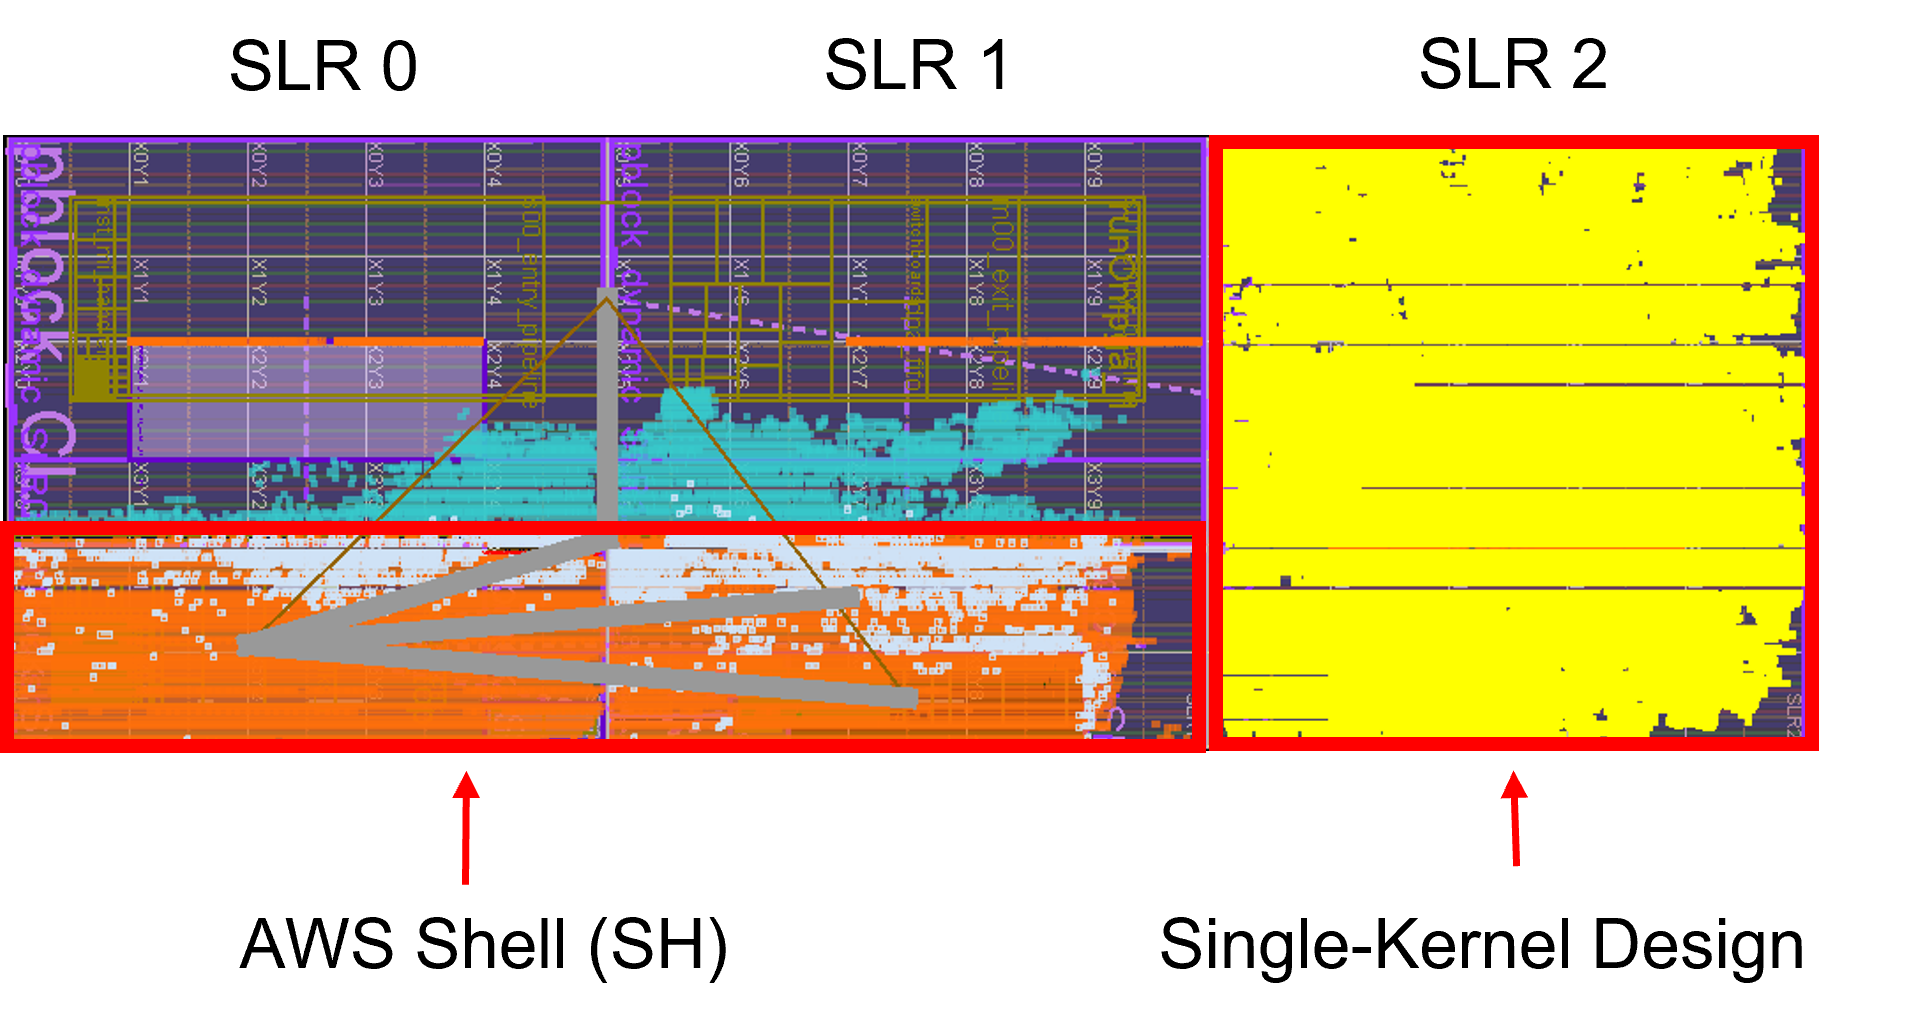
\includegraphics[width=0.6\textwidth]{\graphicsfolder/Figure4.png}
\end{center}
\label{fig:singlekernel}
\small \textit{Note:} Resources utilized by: \textit{(i)} the single-kernel \texttt{CL} design (yellow area); \textit{(ii)} by the AWS shell (orange area); and \textit{(iii)} available \texttt{CL} resources (other colors). The image is captured using Xilinx Vivado.
\end{figure}

\begin{figure}[ht!]
\caption{Three-kernel Design: Resource Utilization}
\begin{center}
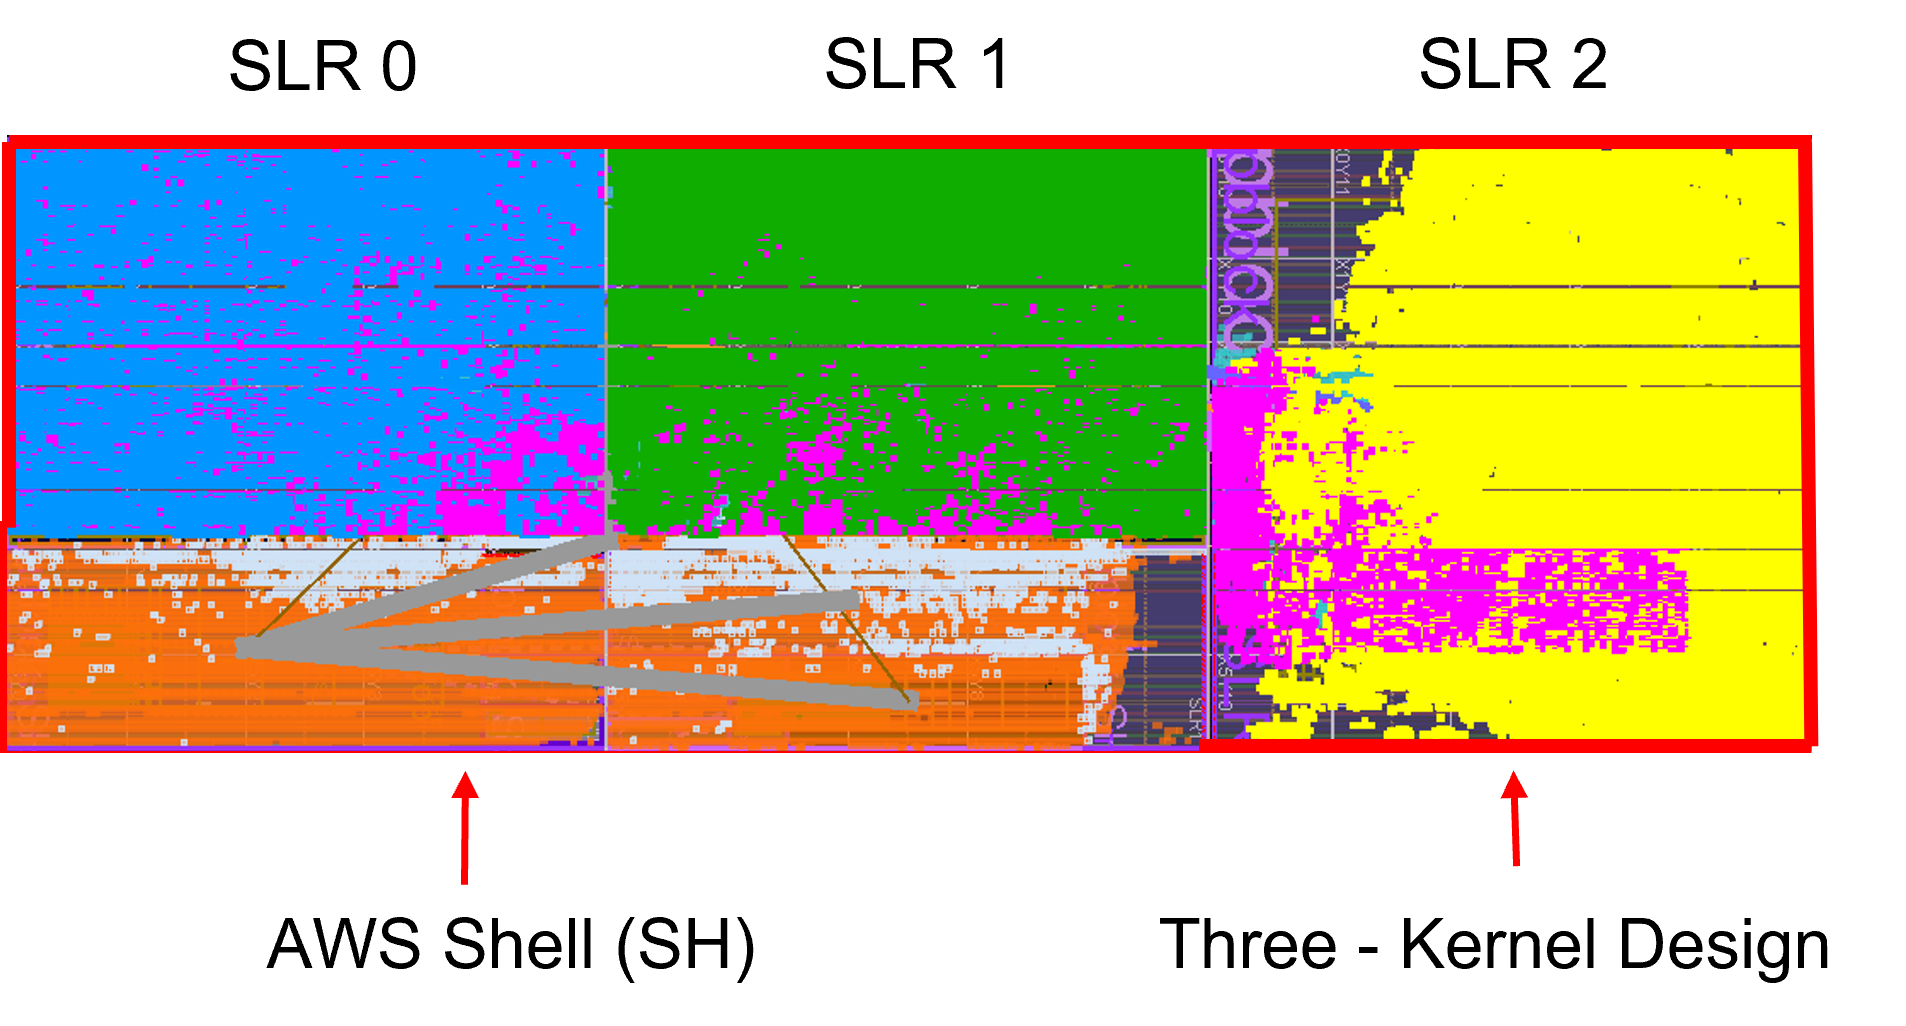
\includegraphics[width=0.6\textwidth]{\graphicsfolder/Figure5.png}
\end{center}
\label{fig:threekernel}
\small \textit{Note:} Resources utilized by: \textit{(i)} the three-kernel \texttt{CL} design (yellow, green, blue areas each corresponding to one kernel); \textit{(ii)} by the AWS shell (orange area); and \textit{(iii)} available \texttt{CL} resources (other colors, of which the pink area serves as a wrapper). The image is created using Xilinx Vivado.
\end{figure}

So, to fit three kernels, we slightly modify our design by reducing the usage of \texttt{CL} resources at the expense of performance. To do so, we provide directives to the compiler to halve the amount of unrolling. In particular, we reduce the unrolling in the \textbf{IHP} design from 2 pipelines working in parallel to a single pipeline. Figure \ref{fig:threekernel} shows the usage of resources associated with the three-kernel design. Hence, we replicate the three-kernel design in each SLR and use \texttt{OpenCL} commands to launch one independent kernel in each of the three SLRs within a single FPGA device (\awsinstfI). The FPGA design becomes \fpgaspeedICPUI times faster than a single-core CPU. Table \ref{tab:baseline} shows how we exploit this parallelism further to deploy more than one FPGA device in parallel on the \awsinstfII and \awsinstfIII instances.


\section{Toward Electrical Engineering Economics}\label{sec:con}

This paper proposes the design of FPGAs for the solution of economic models. This approach requires minimal knowledge of hardware design principles. With small modifications of standard \texttt{C/C++} code, a single FPGA can deliver the same performance as \baselinespeedupFPGAICPUI\hspace{-0.2cm}CPU cores when solving a canonical heterogeneous agent model. The associated energy savings make the compiler approach particularly appealing for organizations with in-house clusters whose computational needs are often constrained by the power limits on the cluster installation and the need to reduce the carbon footprint. 

Our analysis leaves important venues for exploration. First, the recent popularization of machine learning techniques for the solution of economic models (\citealp{fernandez2019financial}, and \citealp{MahdiEbrahimiKahou2021}, among many others) may benefit from decades of research in the electrical engineering literature \citep{Nurvitadhi2017} in terms of the design of efficient FPGAs. A similar argument applies to the acceleration of maximum likelihood estimators.

Second, notice that despite their acceleration potentials, FPGAs (like GPUs) still represent off-the-shelf application-specific integrated circuits (ASICs). Their routing network, logical units, and memory are pre-designed by the manufacturer to be configurable, but they are not customized to serve any particular algorithm. With a growing literature and the development of sophisticated heterogeneous agent models to assess the effect of monetary policy or the economic impact of climate change, we foresee a not-too-distant future where central banks and other policymaking institutions would invest in the design of ASICs specialized in the solution of these models. It is hard to give a precise estimate, but customized silicons could likely improve the current speedup up to three orders of magnitude, with one order of magnitude only due to the faster clock cycle. FPGAs represent a first step in this direction, as they are actively used in the industry to test the functionality of the hardware design of customized chips. Of course, designing and manufacturing these pieces of silicon is not cheap (on the order of tens to hundreds of millions of dollars). Yet, the beneficial effects of a better-informed monetary or climate change policy dwarf these costs.

In conclusion, there is space for a new field, electrical engineering economics, focused on the design of computational accelerators for economics. Our analysis and successful experience in other areas suggest that such a field can provide computational breakthroughs in the years to come. 

\vspace{-0.5cm}
\section*{Acknowledgments}

We thank Yicheng Li (UPenn, Engineering) for the initial implementation of our hardware design. We thank Lucas Ladenburger, Marina Leah McCann, and Paro Suh (CU Boulder, Economics) for outstanding research assistance. We thank Andrew Monaghan and the CU Boulder Research Computing Center for providing valuable insights. We also thank Giuseppe Bruno and Riccardo Russo (Bank of Italy) for testing an early version of the tutorial associated with this paper and Victor Duarte, Mahdi E. Kahou, and Jesse Perla for their comments. This project used: \textit{(i)} the RMACC Summit supercomputer, supported by the National Science Foundation (awards ACI-1532235 and ACI-1532236), CU Boulder and Colorado State University; \textit{(ii)} AWS Credits awarded under the NSF CC* Hybrid Cloud Award OAC-1925766, Research Computing, CU Boulder, 2022. This project was also supported by the Undergraduate Research Experiences for Diversity Grant, 2021, Institute of Behavioral Science, University of Colorado, USA.

\newpage

\bibliographystyle{chicago}
\bibliography{./EEEbibliography}

\newpage

\appendix

\setcounter{figure}{0} \setcounter{table}{0} \setcounter{page}{1}
\renewcommand
\thefigure{A.\arabic{figure}} \renewcommand
\thetable{A.\arabic{table}} \renewcommand \thepage {A.\arabic{page}}

\setcounter{figure}{0} \setcounter{table}{0} \setcounter{page}{1}
\renewcommand
\thefigure{A.\arabic{figure}} \renewcommand
\thetable{A.\arabic{table}} \renewcommand \thepage {A.\arabic{page}}

\section*{Online Appendix for Programming FPGAs for Economics} \label{appendix}

This online appendix adds further details to the main paper. First, we include a table with all the abbreviations that we use for easy reference.

\begin{table}[ht!]
\caption{\textbf{List of Abbreviations}}
\noindent
\begin{footnotesize}
\begin{tabular}{lll}
\toprule
ALM & Aggregate Law of Motion & Algorithm stage \\
AFI & Amazon FPGA Image & CL design implemented on AWS FPGAs \\
AWS & Amazon Web Services & Cloud service \\
.AWSXCLBIN & FPGA executable & Executable to be run on AWS FPGA\\
BRAM & Block RAM  & Local memory \\
CL & Custom logic & FPGA logical units\\ 
CPU & Central processing unit & - \\
DRAM & Dynamic random access memory & Global memory \\
DSP & Digital signal processing unit & Accumulator unit\\
FPGA & Field-programmable gate array& Custom accelerator \\
GPU & Graphics processing unit & Graphics accelerator \\
HLS & High level synthesis & Compiler-based hardware design\\
IEEE754 & Double-precision floating-point standard & Floating-point standard \\
IHP & Individual Household Problem & Algorithm stage\\ 
II & Initiation Interval & \\
LUT & Lookup table & Logical units available for CL design\\
OpenCL & Open Computing Language & \url{https://www.khronos.org/opencl}\\ 
Open MPI & Open message passing interface & \url{https://www.open-mpi.org}\\
PCIe & Peripheral Component Interconnect Express & Bus-connections with host  \\
SLR & Super Logic Region & FPGA CL regions \\
URAM & Ultra RAM & Local memory \\
Xilinx VU9 & FPGA on AWS & - \\
\bottomrule
\end{tabular}
\end{footnotesize}
\label{tab:acronyms}
\end{table}

\section{More on Building Blocks of FPGAs' Optimizations}

Now, we provide additional information on the building blocks of FPGA optimization presented in Section \ref{sec:buiblo}. Subsection \ref{app:rtl} presents the \texttt{RTL} implementation of the accumulator, Subsection \ref{sec:flopre} overviews the arbitrary-precision fixed-point approximation, and Subsection \ref{app:ass:red:tree} delves into the details of implementing an associative reduce tree in hardware.

\subsection{A comparison of RTL and HLS}\label{app:rtl}

The following listing reports the \texttt{RTL} description of the sequential accumulator in Section \ref{sec:acc}. For comparison purposes, we implement it using the \texttt{VHSIC} Hardware Description Language (\texttt{VHDL}), the same \texttt{RTL} language used in \citet{Peri2020}.

\newpage

\begin{lstlisting}[style=vhdlStyle,caption=VHDL description of the Sequential Accumulator,label=lis:seq:RTL]
library IEEE;
use IEEE.STD_LOGIC_1164.ALL;

-- Adder module
entity single_acc is
    generic (
        din_WIDTH : integer := 64;      -- Width of input data
        dout_WIDTH : integer := 64       -- Width of output data
    );
    port (
        clk : in std_logic;                            -- Clock signal
        reset : in std_logic;                          -- Reset signal
        din0, din1 : in std_logic_vector(din_WIDTH-1 downto 0); -- Input data
        dout : out std_logic_vector(dout_WIDTH-1 downto 0) -- Accumulation result
    );
end entity single_acc;

architecture Behavioral of single_acc is
    -- Registers for storing input and output data
    signal din0_buf, din1_buf : std_logic_vector(din_WIDTH-1 downto 0);
    signal dout_buf : std_logic_vector(dout_WIDTH-1 downto 0);
begin
    -- Copy input data from wires to registers
    process(clk)
    begin
        if rising_edge(clk) then
            if reset = '1' then
                din0_buf <= (others => '0');
                din1_buf <= (others => '0');
            else
                din0_buf <= din0;
                din1_buf <= din1;
            end if;
        end if;
    end process;

    -- Perform accumulation
    dout_buf <= din0_buf + din1_buf;

    -- Output the result
    dout <= dout_buf;

end architecture Behavioral;

-- Copy the input stream to BRAM
entity runOnfpga_st_k_RAM_AUTO_1R1W is
    generic (
        DataWidth : integer := 64;   -- Width of data
        AddressWidth : integer := 3; -- Width of address
        AddressRange : integer := 8  -- Range of address
    );
    port (
        address0 : in std_logic_vector(AddressWidth-1 downto 0); -- Address
        ce0 : in std_logic;                              -- Chip enable in
        d0 : in std_logic_vector(DataWidth-1 downto 0);  -- Data in
        we0 : in std_logic;                              -- Write enable in
        q0 : out std_logic_vector(DataWidth-1 downto 0); -- Data out
        reset : in std_logic;                            -- Reset in
        clk : in std_logic                               -- Clock in
    );
end entity runOnfpga_st_k_RAM_AUTO_1R1W;

architecture Behavioral of runOnfpga_st_k_RAM_AUTO_1R1W is
begin
    -- Internal RAM
    (* ram_style = "auto" *) 
    reg [DataWidth-1:0] ram[0:AddressRange-1];

    -- Read and write operations on RAM
    process(clk)
    begin 
        if rising_edge(clk) then
            if reset = '1' then
                for i in ram'range loop
                    ram(i) <= (others => '0');
                end loop;
            else
                if ce0 = '1' then
                    if we0 = '1' then
                        ram(conv_integer(address0)) <= d0; 
                    end if;
                    q0 <= ram(conv_integer(address0));
                end if;
            end if;
        end if;
    end process;

end architecture Behavioral;

-- Top-level module
entity runOnfpga is
    generic (
        AddressRange : integer := 8    -- Number of elements in the array
    );
    port (
        ap_clk : in std_logic;          -- Clock input
        ap_rst : in std_logic;          -- Reset input
        ap_start : in std_logic;        -- Start input
        in_preinit : in std_logic_vector(63 downto 0); -- Initialization input
        ap_done : out std_logic;        -- Done output
        out_r : out std_logic_vector(63 downto 0);    -- Output data
        out_r_ap_vld : out std_logic    -- Output valid signal
    );
end entity runOnfpga;

architecture Behavioral of runOnfpga is
    -- Local signals
    signal accumulation_sum, loaded_data : std_logic_vector(63 downto 0); -- Accumulation and loaded data
    signal adder_result, temp_result : std_logic_vector(63 downto 0);     -- Adder and temporary result
    signal counter : std_logic_vector(3 downto 0) := AddressRange;        -- Counter to track elements
begin
    -- Add reset for the counter
    process(ap_clk, ap_rst)
    begin
        if ap_rst = '1' then
            counter <= "0000";  -- Reset counter
        elsif rising_edge(ap_clk) then
            if ap_start = '1' then
                if counter < AddressRange then
                    counter <= counter + 1;  -- Increment counter
                end if;
            end if;
        end if;
    end process;

    -- Instantiate an adder module
    adder_1 : entity work.single_acc
    generic map (
        din_WIDTH => 64,
        dout_WIDTH => 64
    )
    port map (
        clk => ap_clk,
        reset => ap_rst,
        din0 => accumulation_sum,
        din1 => loaded_data,
        dout => adder_result
    );

    -- Assign din0 from the previous result
    process(ap_clk)
    begin
        if rising_edge(ap_clk) then
            if ap_rst = '1' then
                accumulation_sum <= (others => '0');
            else
                accumulation_sum <= temp_result;
            end if;
        end if;
    end process;

    -- Copy din1 from local BRAM
    process(ap_clk)
    begin
        if rising_edge(ap_clk) then
            loaded_data <= q0;
        end if;
    end process;

    -- Copy the result to the next 
    process(ap_clk)
    begin
        if rising_edge(ap_clk) then
            temp_result <= adder_result;    
        end if;
    end process;

    -- Output the result
    process
    begin
        if counter = "1000" then
            out_r <= accumulation_sum;  -- Assign the accumulated value
            ap_done <= '1';             -- Indicate accumulation done
            out_r_ap_vld <= '1';
        else
            out_r <= (others => '0');   -- Default value when accumulation is not done
            out_r_ap_vld <= '0';
        end if;
    end process;

end architecture Behavioral;
\end{lstlisting}

\subsection{Arbitrary-precision Fixed-point Approximation: An Overview}\label{sec:flopre}

Computers carry out computation on numbers with finite representations. This raises the question of how we adequately approximate the uncountable real numbers. The advent of the IEEE floating-point standard \citep{ieeefp1985} and the readily available microprocessors that implemented it drove convergence to the modern floating-point representations. Most researchers get enough accuracy from the double-precision version of this standard, and they do not need to think carefully about the impact of finite-precision numeric representations for many uses. 

Nonetheless, double-precision costs hardware and energy. Single-precision floating-point remained of interest for energy-conscious signal processing and the highest throughput computations, as did fixed-point representations, where the significance of the bits does not change (i.e., the decimal point remains in a fixed position --it does not ``float''). When custom hardware, both VLSI and FPGAs, is designed, precision optimization remains a point of leverage. For example, in modern Xilinx FPGAs, a double-precision floating-point add can take 700 LUTs, while a 32b fixed-point add only takes 16. A double-precision floating-point multiply takes over 2400 LUTs, while a 32$\times$32 fixed-point multiply is only 1100, and a 16$\times$16 multiply is around 300 \citep{xilinx_fp2020}.  

\subsubsection{Implementation of fixed-point arithmetic in HLS}\label{sec:fixpre}

We refer to \citet{vitis-hls-ug1399} for a guide to the implementation of arbitrary precision in Vitis. 
\clearpage
\begin{figure}[ht!]
\caption{Fixed-point Accumulation Operation}
\begin{center}
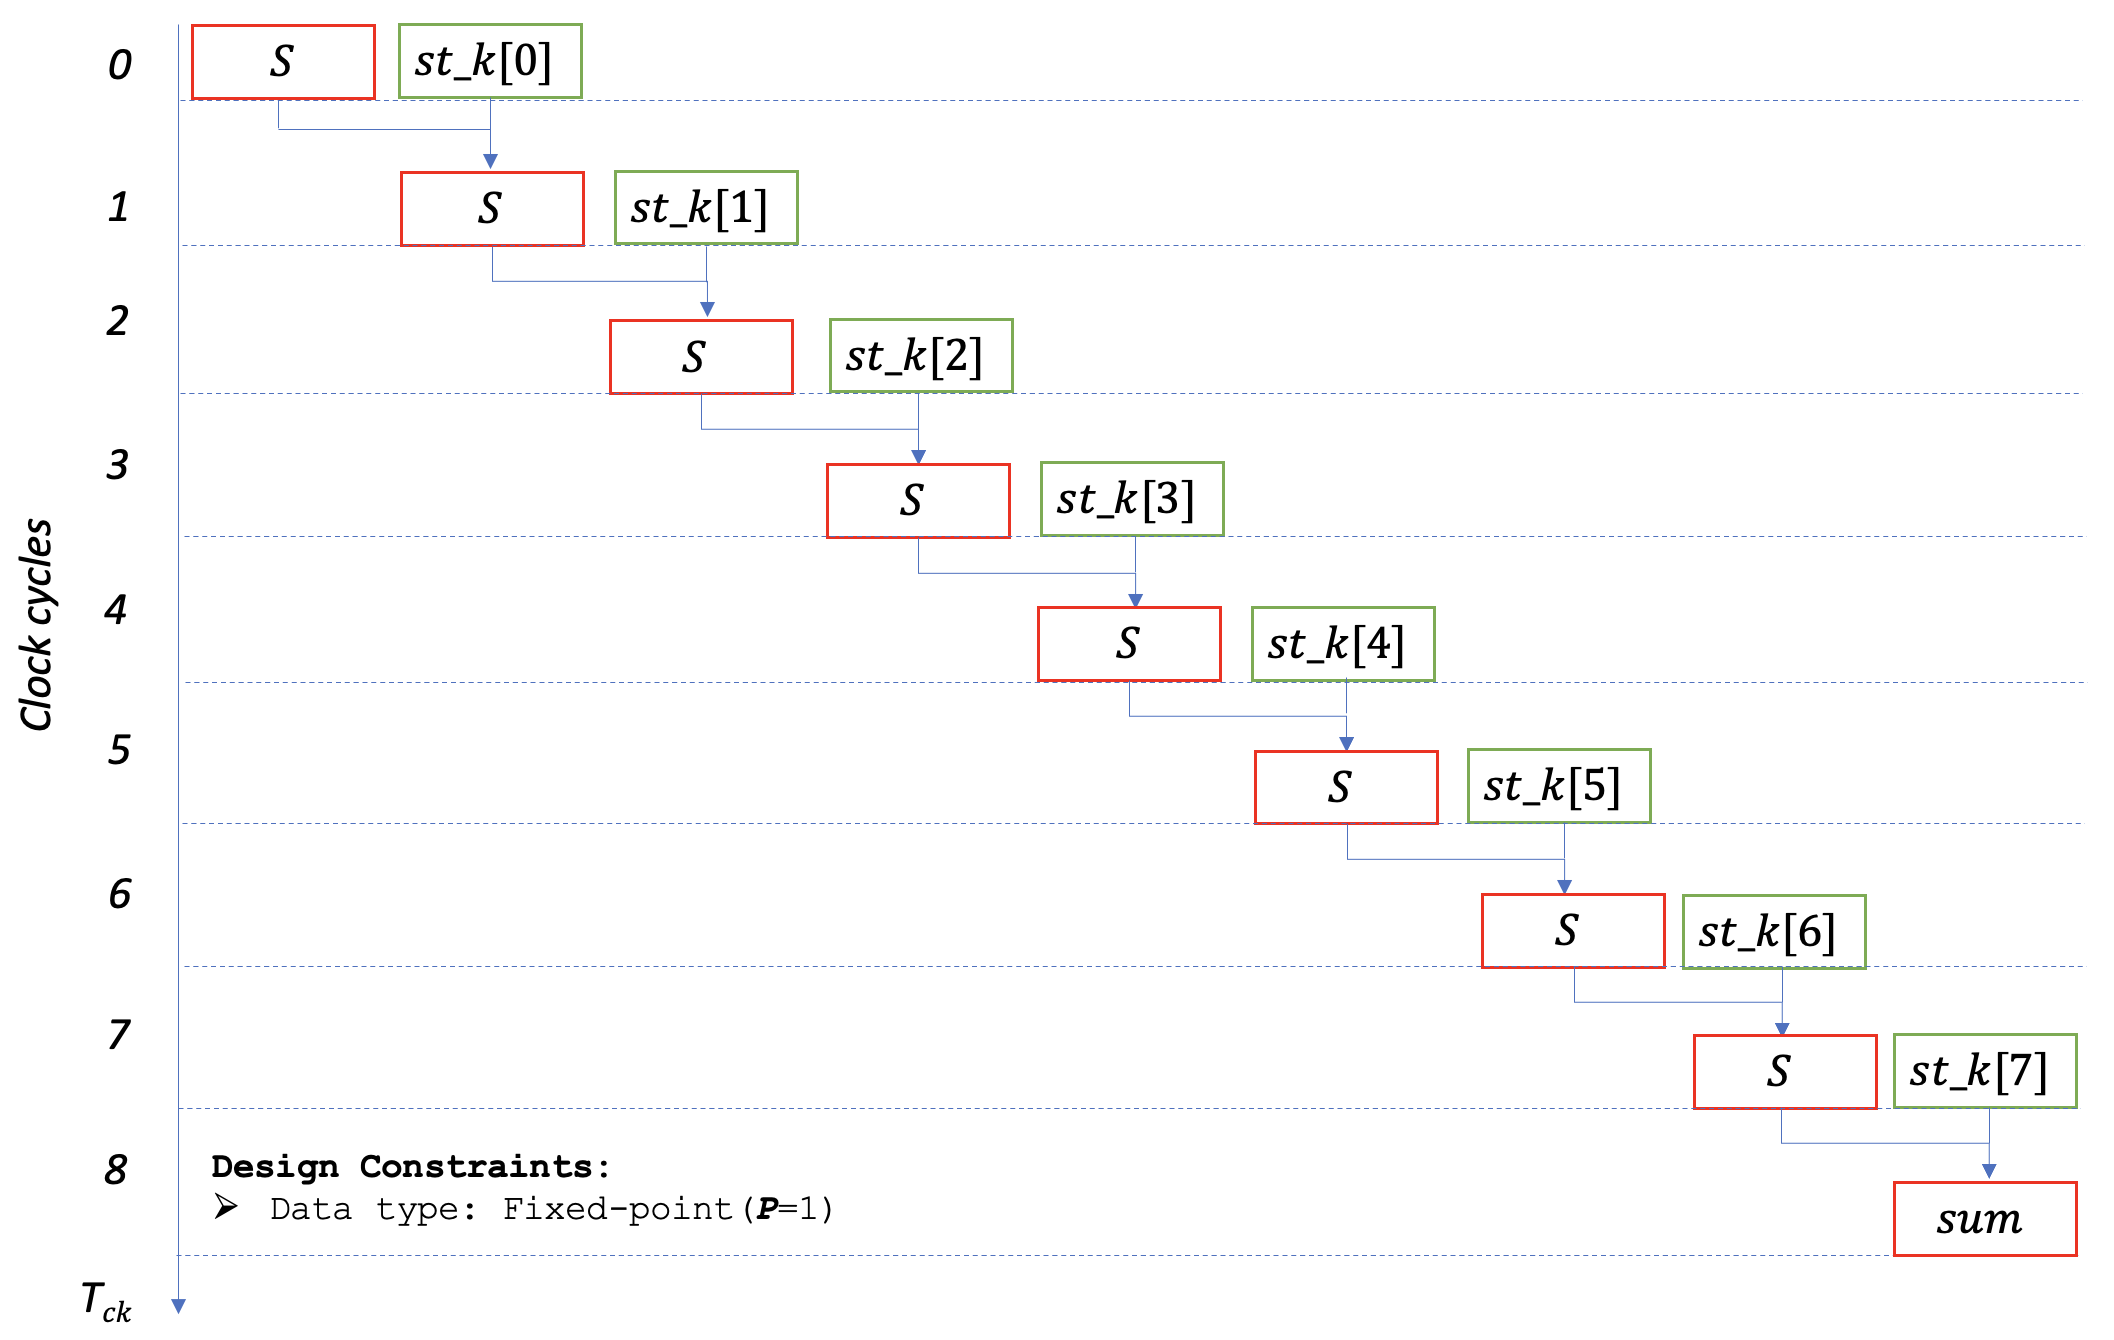
\includegraphics[width=1\textwidth]{\graphicsfolder/FigureA1.png}
\end{center}
\label{fig:acc:fixpre}
\end{figure}

\subsection{Associative Reduce Tree}\label{app:ass:red:tree}

A {\em reduce} operation is a computational construct designed to reduce a large set of numbers into a single value. Common ways to reduce a set of numbers to a single digest include summing them up, multiplying them together, and identifying the maximum or minimum value of the set.
For example, in Subsection \ref{sec:prohls} we consider an add-reduce tree of an array of $N=8$ elements:
\begin{verbatim}
 sum=0;
 for (int i=0;i<8;i++)
    sum+=a[i];
\end{verbatim}
This sequential summation performs $N-1=7$ serial additions operations,
\begin{equation*}
sum=(((((((a[0]+a[1])+a[2])+a[3])+a[4])+a[5])+a[6])+a[7])
\end{equation*}
exactly as illustrated in Figure~\ref{areduce8}(a).

\begin{figure}[!htbp]
\begin{center}
\begin{tabular}{ccc}
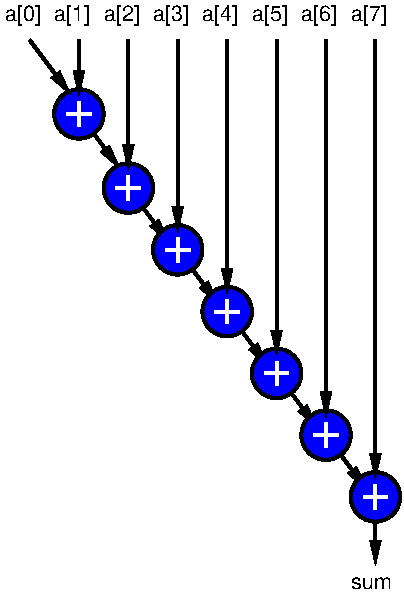
\includegraphics[width=2in]{\graphicsfolder/FigureA2a} & \hspace*{1cm} &
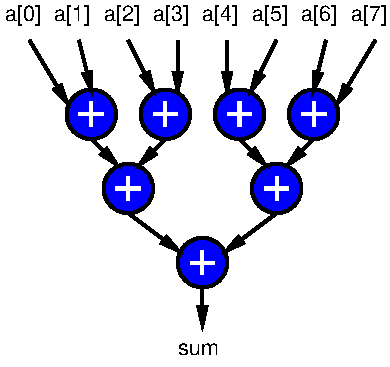
\includegraphics[width=2in]{\graphicsfolder/FigureA2b} \\
(a) Sequential & &  (b) Associative Reduce Tree \\
\end{tabular}
\end{center}
\caption{Associative Reduce Tree Transformation for Sequential
Accumulation}\label{areduce8} 
\end{figure}

When the reduce operation is associative---such as in the case of fixed-precision fixed-point (but not in the case of the IEEE754 double-precision floating-point format, as discussed in Subsection \ref{sec:acc:fix-pre})---we can leverage parallelism to execute the $N-1$ operations in $\log_2 N$ steps.\footnote{The logarithmic base 2 comes from the fact that we use a binary addition operation to digest pairs of numbers at a time.  At each stage, we divide the number of partial sums in half, such that it takes us $\log_2N$ steps to reduce to a single, final sum.  Had we used a $k$-input operator to reduce $k$ numbers to one at each stage, we would need $\log_k N$ steps.} This is achieved by employing a tree structure in which each step (or level in the tree) successively reduces the number of values by half through pair-wise combinations,
\begin{equation*}
sum=(((a[0]+a[1])+(a[2]+a[3]))+((a[4]+a[5])+(a[6]+a[7])))
\end{equation*}
as illustrated in Figure~\ref{areduce8}(b). Given adequate hardware, an associative reduce tree (Figure~\ref{areduce8}(b)) can perform $N-1=7$ operations in $\log_2 N=3$ sequential steps (also referred to as the \textit{depth} of the tree). 

\subsubsection{Memory-access bottleneck in absence of array partitioning}\label{sec:membot}

Figure \ref{fig:acc:fix:unroll8:fail} shows the data flow of an accumulator with loop unroll and no array partitioning. This is a circuit that tries to unroll by a factor of 8 the addition of the fixed-point elements of an array \texttt{st\_k} of size $\Naccsize=8$. The vertical dimension illustrates in which clock cycles these operations are performed (\textit{scheduling}). The circuit fails to execute the prescribed unrolling because of a memory reading conflict that prevents reading more than two elements from the same BRAM.

\begin{figure}[ht!]
\caption{Data Flow of Accumulator with Loop Unroll (No Array Partitioning)}
\begin{center}
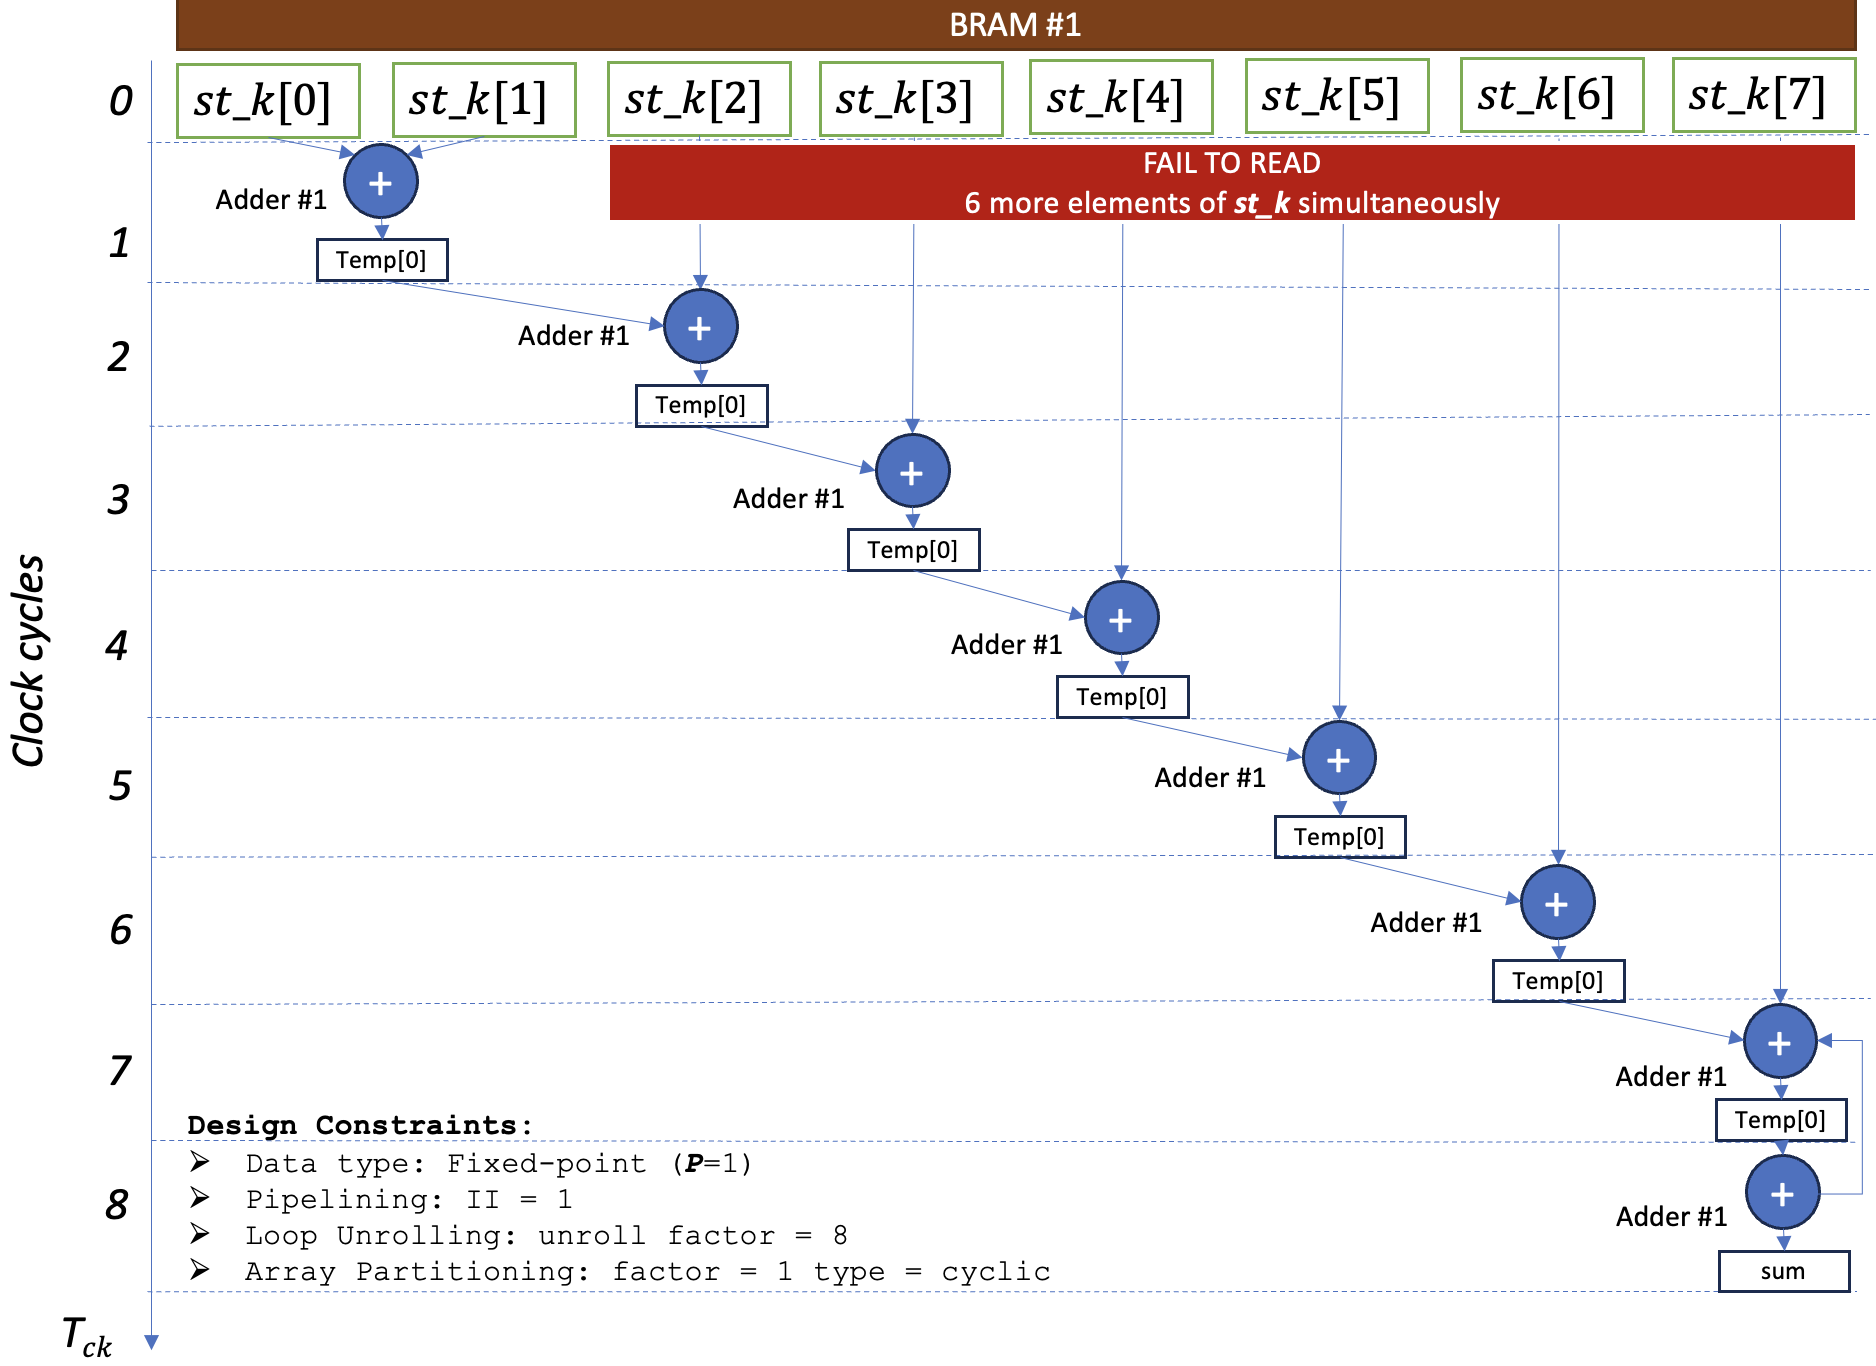
\includegraphics[width=0.9\textwidth]{\graphicsfolder/FigureA3.png}
\end{center}
\label{fig:acc:fix:unroll8:fail}
\end{figure}

\section{AWS Instances Technical Specs}\label{sec:aws:tecspe}

\begin{table}[ht!]
\begin{center}
\caption{Technical Specifications}
\begin{tabular}{l c c c c}
\toprule
\textbf{AWS Instance} & \textbf{Cores} & \textbf{FPGAs} & \textbf{Pricing} (\$/hour) & \textbf{Memory} (GiB) \\ 
\midrule
\cpuI & 1 & - & 0.119 & 8\\
\cpuII & 8 & - & 0.952 & 64\\
\cpuIII & 48 & - & 5.712 & 384\\
\awsinstfI & 4 & 1 & 1.650 & 122\\
\awsinstfII & 8 & 2 & 3.300 & 244\\
\awsinstfIII & 32 & 8 & 13.200 & 976\\
\bottomrule
\label{tab:tecspe}
\end{tabular}
\end{center}
\small
\noindent \textit{Note:} Hardware architecture and AWS cloud pricing (Columns 2-5) for deployed AWS instances (Column 1). The column marked Cores reports the number of physical cores. The column marked FPGAs reports the number of connected FPGA chips (f1 instances only). The column marked Pricing denotes the AWS \textit{On Demand} Pricing per instance per hour as of September 2021. Memory is measured in Gigabytes. \textit{Source:} \href{https://aws.amazon.com/ec2/instance-types/}{AWS instances}, \href{https://docs.aws.amazon.com/AWSEC2/latest/UserGuide/cpu-options-supported-instances-values.html}{AWS specs}.
\end{table}

\noindent \textbf{M5N Instances.} \textit{(a) CPU:} Intel Xeon Scalable Processors (Cascade Lake, 2nd generation), with sustained all-core Turbo CPU frequency of 3.1 GHz, maximum single-core Turbo CPU frequency of 3.5 GHz;
\textit{(b) Network Bandwidth:} up to 25 Gbps;
\textit{(c) Storage} EBS.

\textit{Remark.} We select M5N instances for three reasons. First, their architecture roughly belongs to the same vintage as our FPGAs --with the Xilinx VU9P being released a little bit earlier (2016) than the Intel Xeon Scalable Processor (Cascade Lake, second generation, 2019) featured in M5N instances-- thus, allowing us to control for technological improvements.
Second, these CPUs compare favorably with respect to CPUs available in state-of-the-art supercomputers, for instance, the Intel Xeon E5-2680 v3 @2.50GHz (2 CPUs/node, 24 cores/node) provided by the CU Boulder RMACC Summit supercomputer. As a result, they provide a good benchmark of the expected performance. Third, they are the Amazon AWS general-purpose instances with the largest number of cores (as of 2022); hence, they enable meaningful multi-core parallelism while preserving comparability. 

\noindent \textbf{F1 Instances.} 
\textit{(a) CPU:} Intel Xeon E5-2686 v4 Processor, with a base CPU frequency of 2.3 GHz and Turbo CPU frequency of 2.7 GHz.
\textit{(b) Network Bandwidth:} up to 10 Gbps for f1.2xlarge and f1.4xlarge, and 25 Gbps for f1.16xlarge.
\textit{(c) Storage} 
\textit{f1.2xlarge}: 470 GiB NVMe SSD
\textit{f1.4xlarge}: 940 GiB NVMe SSD
\textit{f1.16xlarge}: 3760 GiB (4 \* 940 GiB NVMe SSD).\\
\textit{Source:} For further information, visit \href{https://aws.amazon.com/ec2/instance-types/}{https://aws.amazon.com/ec2/instance-types/}.

\section{Hardware Designs: Resources and Performance}\label{app:perf}

We now report resource utilization and performance measures associated with the hardware designs discussed in the main paper.

\subsection{FPGA Designs Performance and Resource Utilization}\label{app:resuti}

First, Table \ref{Tab:resourse_grid} reports time performance and resource utilization by hardware design.

\begin{table}[ht!]
\caption{FPGA Designs Performance and Resource Utilization by Grid Size}
\vspace{-0.1in}
\begin{center}
\begin{footnotesize}
\begin{tabular}{lccccccccc}
\toprule
&\textbf{Three-Kernel}&&\multicolumn{7}{c}{\textbf{Single-Kernel}} \\
\cmidrule{2-2}\cmidrule{4-10}
\multicolumn{1}{l}{\text{Aggr. Capital}} &\textit{4}&& \multicolumn{3}{c}{\textit{4}} && \multicolumn{3}{c}{\textit{8}}\\
\cmidrule{2-2}\cmidrule{4-6}\cmidrule{8-10}
\multicolumn{1}{l}{\text{Indiv. Capital}} &\textit{100}&& \textit{100}&\textit{200}&\textit{300}&& \textit{100}&\textit{200}&\textit{300}\\
\cmidrule{2-2}\cmidrule{4-6}\cmidrule{8-10}
Time (s) &\fpgaItime &&\fpgatimeIknlInKMIkI & \fpgatimeIknlInKMIkII & \fpgatimeIknlInKMIkIII && \fpgatimeIknlInKMIIkI & \fpgatimeIknlInKMIIkII & \fpgatimeIknlInKMIIkIII\\  
Cost (\$)& \fpgaIcost && \fpgacostIknlInKMIkI & \fpgacostIknlInKMIkII & \fpgacostIknlInKMIkIII && \fpgacostIknlInKMIIkI & \fpgacostIknlInKMIIkII & \fpgacostIknlInKMIIkIII\\
Energy (J)& \fpgaIenergy &&  \fpgaenergyIknlInKMIkI & \fpgaenergyIknlInKMIkII & \fpgaenergyIknlInKMIkIII && \fpgaenergyIknlInKMIIkI & \fpgaenergyIknlInKMIIkII & \fpgaenergyIknlInKMIIkIII\\
BRAM(\%)&\acrossdataparallelBRAM&&\bramnKMIkI & \bramnKMIkII & \bramnKMIkIII && \bramnKMIIkI & \bramnKMIIkII & \bramnKMIIkIII\\
DSP(\%)&\acrossdataparallelDSP&&\dspnKMIkI & \dspnKMIkII & \dspnKMIkIII && \dspnKMIIkI & \dspnKMIIkII & \dspnKMIIkIII\\
Registers(\%)&\acrossdataparallelRegisters&&\registernKMIkI & \registernKMIkII & \registernKMIkIII && \registernKMIIkI & \registernKMIIkII & \registernKMIIkIII\\
LUT(\%)&\acrossdataparallelLUTs&&\lutnKMIkI & \lutnKMIkII & \lutnKMIkIII && \lutnKMIIkI & \lutnKMIIkII & \lutnKMIIkIII\\
URAM(\%)&\acrossdataparallelURAM&&\uramnKMIkI & \uramnKMIkII & \uramnKMIkIII && \uramnKMIIkI & \uramnKMIIkII & \uramnKMIIkIII\\
\bottomrule
\end{tabular}
\end{footnotesize}
\label{Tab:resourse_grid}
\end{center}
\label{tab:res}
\small \textit{Note:} Solution time (in seconds), cost (in USD), energy (in joules) and FPGA resources (rows) across hardware designs (three- and single-kernel) and grid sizes on individual capital $N_{k}=\{100,200,300\}$ and aggregate capital $N_{M}=\{4,8\}$ (columns). Time performance is measured in seconds required to solve \numbeconII baseline economies on a single FPGA (\awsinstfI) across the different hardware designs and grid sizes (columns). Resources are measured (using Xilinx Vivado) as a percentage of Xilinx VU9P FPGA's resources utilized by AWS images associated with the different hardware designs and grid sizes (columns). \textit{Available Resources:} BRAM (\CLdesignBRAM), DSP (\CLdesignDSP), Registers (\CLdesignRegisters), LUTs (\CLdesignLUT), URAM (\CLdesignURAM). Available resources are lower than total resources because they exclude resources utilized by the AWS shell that are not available for \texttt{CL} design.
\end{table}

\subsection{Efficiency Gains of Benchmark Economy}\label{app:effgai}

Next, Table \ref{tab:perf_comp} reports the performance of different FPGA hardware designs and CPU-core platforms that yield the efficiency gains reported in the paper in terms of execution speedup, AWS costs, and energy savings.

\begin{table}[ht!]
\caption{Performance Comparison}\label{tab:perf_comp}
\vspace{-0.2in}
\hspace{-1.8cm} 
\begin{center}
\begin{tabular}{lccccccc}
\toprule
&\multicolumn{3}{c}{\textbf{CPU cores}}&&\multicolumn{3}{c}{\textbf{FPGA devices}}\\
\cmidrule{2-4}\cmidrule{6-8}
N.    &1&8&48&&1&2&8\\
\cmidrule{2-4}\cmidrule{6-8}
Exec Time (s) &\cpuItimetot &\cpuIItimetot &\cpuIIItimetot && \fpgaItimetot &\fpgaIItimetot &\fpgaIIItimetot\\
Init Time (s) &\cpuIinittime &\cpuIIinittime &\cpuIIIinittime&&  \fpgaIinittime&\fpgaIIinittime&\fpgaIIIinittime\\         
Print Time (s) &\cpuIwritetime &\cpuIIwritetime &\cpuIIIwritetime&& \fpgaIwritetime&\fpgaIIwritetime&\fpgaIIIwritetime\\     
Sol. Time (s) &\cpuItime &\cpuIItime &\cpuIIItime&& \fpgaItime&\fpgaIItime&\fpgaIIItime\\
Cost (\$) & \cpuIcost & \cpuIIcost &\cpuIIIcost && \fpgaIcost&\fpgaIIcost&\fpgaIIIcost\\
Energy (J) & \cpuIenergy& \cpuIIenergy &\cpuIIIenergy&& \fpgaIenergy&\fpgaIIenergy&\fpgaIIIenergy\\
\cmidrule{2-8}
AWS Instance & \cpuI & \cpuII  & \cpuIII &&\awsinstfI&\awsinstfII&\awsinstfIII \\  
\bottomrule         
\end{tabular}
\end{center}
\small
\textit{Note:} Execution, initialization, printing and solution time (in seconds), cost (in USD) and energy (in joules) to solve \numbeconII baseline economies using \texttt{Open MPI} CPU multi-core acceleration on Amazon M5N multi-core instances (with 1, 8, 48 physical cores, Columns 1-3) and using FPGA acceleration on Amazon F1 instances (connected to 1, 2, 8 FPGA devices, Columns 4-6). 
\end{table}

Differences in the execution time of initialization and printing operations between FPGA and CPU experiments are attributed to their parallel execution via \texttt{Open MPI} on the CPU experiments and sequential execution on the CPU (host side) of the FPGA accelerated experiments. These differences can be eliminated by using \texttt{Open MPI} on the host side of the FPGA experiments. The FPGA has extra time allocation costs due to the OpenCL initialization of host/device communications. Crucially, the relative magnitude of the non-kernel operations time washes out as the number of economies increases. Not surprisingly, the relative time spent on non-kernel operations disproportionately affects the experiment with 8 FPGAs, where non-kernel tasks account for roughly \fpgaIIIlossExecvsKernelTime\% of the total execution time. These results suggest that the use of 8 FPGAs may be more cost-effective when executing a large amount of economies in parallel.

\subsubsection{Energy consumption} \label{app:pow} 

The FPGA power consumption is measured using the AFI management tool command\\ \textcolor{blue}{\lstinline{sudo fpga-describe-local-image -S 0 -M}}. To make our energy performance comparison as meaningful as possible, we select the FPGA average power consumption (across all our experiments, including different capital grids), which amounted to \fpgaIpowerconsumption\, watts per FPGA device.

The CPU power consumption can be determined using the Turbostat application.\footnote{Source: \href{https://www.linux.org/docs/man8/turbostat.html}{https://www.linux.org/docs/man8/turbostat.html}.} However, Turbostat does not work on Amazon M5N instances. As a workaround:

\begin{itemize}

\item We use Turbostat to measure the power consumption of our application on the Amazon AWS metal instance.

\item We then compare this number with the Thermal Design Power (TDP).\footnote{Source: \href{https://www.intel.com/content/www/us/en/support/articles/000055611/processors.html}{https://www.intel.com/content/www/us/en/support/articles/000055611/processors.html}.} The comparison between the Turbostat application and the TDP establishes that our application requires approximately the maximum CPU power.
\end{itemize}
We map this estimate into our M5N instances with 1, 8, and 48 cores using the formula:
\begin{equation*}
\text{Power M5N}(\text{cores}) = \frac{\text{cores}}{\text{cores}_{\text{Metal}}}*\text{Power Turbostat},\qquad \text{cores}\in\{1,8,48\}. 
\end{equation*}
We estimate a power consumption of \cpuIpowerconsumption\ watts per CPU core. To get the energy, we compute:
\begin{equation*}
\text{Energy M5N}(\text{cores}) = \text{Power M5N}(\text{cores})\cdot \text{Time}(\text{cores}),\qquad \text{cores}\in\{1,8,48\}.
\end{equation*}

\subsection{CPU Performance Across Grid Sizes}\label{app:gri} 

Finally, Table \ref{Tab:grid_sizes} reports the CPU performance across different sizes of the grid.

\begin{table}[ht!]
\caption{CPU Performance by Grid Size}
\begin{center}
\begin{footnotesize}
\begin{tabular}{lccccccccc}
\toprule
\multicolumn{1}{l}{\text{Aggregate Capital}, $N_M$} && \multicolumn{3}{c}{\textit{4}} && \multicolumn{3}{c}{\textit{8}}\\
\cmidrule{3-5}\cmidrule{7-9}
\multicolumn{1}{l}{\text{Individual Capital}, $N_k$} && \textit{100}&\textit{200}&\textit{300}&& \textit{100}&\textit{200}&\textit{300}\\
\cmidrule{3-5}\cmidrule{7-9}
Exec. Time (s) &&\cpuIKMIkItimetot&\cpuIKMIkIItimetot&\cpuIKMIkIIItimetot&&\cpuIKMIIkItimetot&\cpuIKMIIkIItimetot&\cpuIKMIIkIIItimetot\\
Init. Time (s) &&\cpuIKMIkIinittime&\cpuIKMIkIIinittime&\cpuIKMIkIIIinittime&&\cpuIKMIIkIinittime&\cpuIKMIIkIIinittime&\cpuIKMIIkIIIinittime\\
Print Time (s) &&\cpuIKMIkIwritetime&\cpuIKMIkIIwritetime&\cpuIKMIkIIIwritetime&&\cpuIKMIIkIwritetime&\cpuIKMIIkIIwritetime&\cpuIKMIIkIIIwritetime\\
Sol. Time (s) && \cpuIKMIkItime&\cpuIKMIkIItime&\cpuIKMIkIIItime&& \cpuIKMIIkItime&\cpuIKMIIkIItime&\cpuIKMIIkIIItime\\
Cost (\$) && \cpuIKMIkIcost & \cpuIKMIkIIcost& \cpuIKMIkIIIcost && \cpuIKMIIkIcost & \cpuIKMIIkIIcost& \cpuIKMIIkIIIcost\\
Energy (J) && \cpuIKMIkIenergy & \cpuIKMIkIIenergy & \cpuIKMIkIIIenergy&& \cpuIKMIIkIenergy & \cpuIKMIIkIIenergy & \cpuIKMIIkIIIenergy\\
\bottomrule         
\end{tabular}
\end{footnotesize}
\end{center}
\label{Tab:grid_sizes}
\small
\textit{Note:} Execution, initialization, printing and solution time (in seconds), cost (in USD) and energy (in joules) to solve \numbeconII baseline economies on a single core CPU (\cpuI) for different grid sizes (columns) on individual capital $N_{k}=\{100,200,300\}$ and aggregate capital $N_{M}=\{4,8\}$.
\end{table}

\subsection{Precision Accuracy Analysis}\label{app:preaccana}

This section reports the accuracy analysis associated with FPGA and CPU implementation of the \cite{KrusellSmith1998} algorithm.

\begin{table}[htb!]
\setlength\tabcolsep{0pt}
\caption{Precision Accuracy Analysis}
\vspace{-0.1in}
\begin{center}
\begin{subtable}{\textwidth}
\caption{ALM Coefficients}
\begin{tabular*}{\textwidth}{@{\extracolsep{\fill}} l *{5}{c} }
\toprule
&$\beta_{1}(a_b)$&$\beta_{2}(a_b)$&$\beta_{1}(a_g)$&$\beta_{2}(a_g)$\\
\cmidrule{2-5}
Floating-Point &\betaIab&\betaIIab&\betaIag&\betaIIag\\
Fixed Point &\betaIabFix&\betaIIabFix&\betaIagFix&\betaIIagFix\\
\bottomrule
\end{tabular*}
\end{subtable}
\par\bigskip
\begin{subtable}{\textwidth}
\caption{Policy Function, $k'$}
\begin{tabular*}{\textwidth}{@{\extracolsep{\fill}} l *{6}{c} }
\toprule
Mean$\left(\frac{|\text{Fixed}-{Float}|}{Float}\right)\%$&\absmeandifferencekprime&&&Max$\left(\frac{|\text{Fixed}-{Float}|}{Float}\right)\%$ &\absmaxdifferencekprime\\
\bottomrule
\end{tabular*}
\end{subtable}
\par\bigskip
\begin{subtable}{\textwidth}
\caption{Individual Capital Holdings Distribution, $T=1,100$}
\begin{tabular*}{\textwidth}{@{\extracolsep{\fill}} l *{6}{c} }
\toprule
&Mean & Std& 0.25 & 0.5 & 0.75\\
\cmidrule{2-6}
Floating-Point &\meankcross&\stdkcross&\qIkcross&\mediankcross&\qIIIkcross\\
Fixed Point &\meankcrossFix&\stdkcrossFix&\qIkcrossFix&\mediankcrossFix&\qIIIkcrossFix\\
\midrule
Mean$\left(\frac{|\text{Fixed}-{Float}|}{Float}\right)\%$&\absmeandifferencekcross&&&Max$\left(\frac{|\text{Fixed}-{Float}|}{Float}\right)\%$ &\absmaxdifferencekcross\\
\bottomrule
\end{tabular*}
\end{subtable}
\begin{subtable}{\textwidth}
\caption{Euler Equation Errors (EEE)}
\label{tab:EE} 
\begin{tabularx}{\textwidth}{XXXXX}
\toprule
&   EEE   & FPGA & CPU & $|\Delta_{\text{FPGA}-\text{CPU}}/\text{CPU}|$\% \\
\cmidrule{2-5}
\multirow{2}{*}{$N_k=100$} &  Mean (\%)  & \EEEmeanfpgaIKMIkI & \EEEmeancpuIKMIkI & \EEEmeanrelKMIkI\\
&Max (\%)  & \EEEmaxfpgaIKMIkI & \EEEmaxcpuIKMIkI & \EEEmaxrelKMIkI\\
\multirow{2}{*}{$N_k=300$} & Mean (\%)  & \EEEmeanfpgaIKMIkIII & \EEEmeancpuIKMIkIII & \EEEmeanrelKMIkIII\\
&Max (\%)   & \EEEmaxfpgaIKMIkIII & \EEEmaxcpuIKMIkIII & \EEEmaxrelKMIkIII\\      
\bottomrule
\end{tabularx}
\end{subtable}
\end{center}
\label{tab:preana}
\end{table}

Panel A of Table \ref{tab:preana} reports the equilibrium ALM coefficients $\hat{b}(a)=(\hat{b}_1(a),\hat{b}_2(a))$ with $a\in\{a_b,a_g\}$ under floating- and fixed-point in the FPGA and CPU, respectively. Panel B reports the mean and max relative difference (in percent) between the policy functions computed under floating- and fixed-point. Panel C reports moments of the distribution of individual capital holdings at $T=1,100$ (mean, standard deviation, and quartiles) under floating- and fixed-point. The last row reports their mean and max relative difference in percent. Panel D reports the mean/max Euler equation errors expressed in percent, associated with policy functions estimated in fixed-point using the FPGA (column 2), in floating-point on the CPU (column 3), and relative absolute difference, all in percent, for different individual capital holdings grid sizes, $N_k \in\{100,300\}$ (rows), with $N_M=4$.

\section{Carbon Footprint of Scientific Computing}\label{sec:carfot}

This appendix proposes a back-of-the-envelope calculation in order to estimate the carbon footprint of the Summit and Blanca Supercomputers. Calculations have been provided by independent research at the CU Boulder Research Computing Center and updated to 2020 data.\footnote{Andrew Monaghan, \href{mailto:  Andrew.Monaghan-1@Colorado.EDU}{Andrew.Monaghan-1@Colorado.EDU}.} 

The RC analysis assumes that each CURC HPC core consumes $13$W, that is, 0.013 kilowatts per CURC HPC core hour ($13 \text{W/core} \cdot 1 \text{hour} /1000 = 0.013 kWh$). It then uses the Xcel Energy power generation breakdown in the state of Colorado in 2020\footnote{\textit{Source:} Xcel Stats, \href{https://co.my.xcelenergy.com/s/energy-portfolio/power-generation}{https://co.my.xcelenergy.com/s/energy-portfolio/power-generation}.} --37\% Natural Gas, 26\% Coal, 37\% Renewables-- and US EPA information on the emissions of CO$_2$ per kWh by source\footnote{\textit{Source:} US EPA \href{https://www.eia.gov/tools/faqs/faq.php?id=74&t=11}{ https://www.eia.gov/tools/faqs/faq.php?id=74\&t=11}.} --0.91 Natural Gas, 2.21 Coal, 0.1 Renewables\footnote{This estimate is not given. The original analysis assumes it to be 0.1 for externalized carbon.}-- to determine the average pounds of CO$_2$ per Xcel Colorado kWh:
\begin{equation*}
0.37*0.91 + 0.26*2.21 + 0.37*.1 = 0.9483 \,\frac{\text{lbs CO$_2$}}{\text{kWh}}
\end{equation*}
Putting this information together, it estimates 0.0123 pounds CO$_2$ per CURC HPC core per hour:
\[0.9483 \,\frac{\text{lbs CO$_2$}}{\text{kWh}} * 0.013 \,\frac{\text{kWh}}{\text{core hour}} = 0.0123\,\frac{\text{lbs CO$_2$}}{\text{core hour}},\] On average the Summit and Blanca supercomputers (CU Boulder) serve $150$ million core hours per year and therefore produce on average \[150\cdot10^6\, \frac{\text{core hour}}{\text{year}} \cdot 0.0123 \,\frac{\text{lbs CO$_2$}}{\text{core hour}} = 1,849,185 \, \frac{\text{lbs CO$_2$}}{{\text{year}}}, \] which corresponds to \SummittotmTonCOII\, metric tons of CO$_2$ per year. To put this number in context, a typical US car emits about five metric tons per year. So, the annual Summit and Blanca carbon footprint is roughly the same as that of $\SummittotmTonCOII/5\approx\cpucarsnumber$ cars per year.

To explore the carbon footprint impact of moving all of these CPU-intensive computations to FPGA devices, let us assume an FPGA power consumption similar to the one measured on the Xilinx VU9P of \fpgaIpowerconsumptionperhour\, kWh per FPGA per hour. Accordingly, \[0.9483 \,\frac{\text{lbs CO$_2$}}{\text{kWh}} * \fpgaIpowerconsumptionperhour\,\frac{\text{kWh}}{\text{FPGA hour}} = \fpgaICOIIpoundsperhour \,\frac{\text{lbs CO$_2$}}{\text{FPGA hour}}.\] If (a big if) we assume an acceleration similar to the one measured in our application (\fpgaspeedICPUI\hspace{-0.1cm}x), the 150 million core hours per year would map into $\SummitonFPGAtothours$ FPGA hours per year. In this scenario, the carbon footprint would total:
\[\SummitonFPGAtothours \,\frac{\text{FPGA hour}}{\text{year}} \cdot \fpgaICOIIpoundsperhour \,\frac{\text{lbs CO$_2$}}{\text{FPGA hour}} = \SummitonFPGAtotlbsCOII \, \frac{\text{lbs CO$_2$}}{{\text{year}}}\] or approximately \SummitonFPGAtotmTonCOII \ metric tons of CO$_2$ per year. This is equivalent to a reduction in the carbon footprint from \cpucarsnumber \ cars to \fpgacarsnumber \  cars per year.

\end{document}
 
